\documentclass[12pt,a4paper]{ctexart}
\usepackage[margin=2.2cm]{geometry}
\usepackage{graphicx}
\usepackage{booktabs}
\usepackage{amsmath}
\usepackage{float}
\usepackage{hyperref}
\usepackage{xcolor}
\usepackage{listings}

% SQL 代码样式
\lstdefinestyle{sqlstyle}{
  language=SQL,
  basicstyle=\ttfamily\footnotesize,
  keywordstyle=\color{blue!80!black}\bfseries,
  commentstyle=\color{gray}\itshape,
  stringstyle=\color{orange!70!black},
  showstringspaces=false,
  breaklines=true,
  frame=single,
  tabsize=2,
  morekeywords={IF,EXISTS,COALESCE,LIKE,BETWEEN,OFFSET,LIMIT,
    VIEW,TRIGGER,FUNCTION,RETURNS,LANGUAGE,PLPGSQL,BEGIN,END,
    OLD,NEW,EXECUTE,PROCEDURE,FOR,EACH,ROW,AFTER,BEFORE,
    CREATE,OR,REPLACE,ANALYZE,EXPLAIN,BUFFERS,ON,CONFLICT,
    DO,NOTHING,CASCADE,REFERENCES,INDEX,PARTIAL,VACUUM,
    BOOLEAN,DATE,TIMESTAMP,DECIMAL,NUMERIC,VARCHAR,INT,
    CURRENT_DATABASE,CURRENT_USER,VERSION,NOW,RANDOM}
}

% Java 代码样式
\lstdefinestyle{javastyle}{
  language=Java,
  basicstyle=\ttfamily\footnotesize,
  keywordstyle=\color{blue!80!black}\bfseries,
  commentstyle=\color{gray}\itshape,
  stringstyle=\color{orange!70!black},
  showstringspaces=false,
  breaklines=true,
  frame=single,
  tabsize=4
}

% Python 代码样式
\lstdefinestyle{pythonstyle}{
  language=Python,
  basicstyle=\ttfamily\footnotesize,
  keywordstyle=\color{blue!80!black}\bfseries,
  commentstyle=\color{gray}\itshape,
  stringstyle=\color{orange!70!black},
  showstringspaces=false,
  breaklines=true,
  frame=single,
  tabsize=4
}

\lstset{style=sqlstyle}

\newcommand{\reporttitle}{数据库系统实验报告}
\newcommand{\authname}{姓名}
\newcommand{\authid}{学号}
\newcommand{\class}{班级}

\title{\reporttitle}
\author{\authname：\underline{李祥熙} \quad \authid：\underline{2234412799} \quad \class：\underline{计算机2301}}
\date{\today}

\begin{document}
\maketitle
\tableofcontents
\newpage

% ===== 一、实验目的 =====
\section{实验目的}

本实验以 openGauss 关系型数据库管理系统为实验平台，通过构建学生选课数据库，系统性地训练数据库系统的核心操作能力，具体目标如下：

\begin{itemize}
  \item \textbf{掌握数据定义与数据操纵基本操作}：能够独立创建数据库与表结构，合理选择各属性的数据类型，并完成数据的录入、查询、修改和删除操作。
  \item \textbf{提升复杂 SQL 查询编写能力}：通过编写涵盖子查询、聚合函数、分组过滤、多表连接、分页查询等多种语法的 SQL 语句，深入理解关系代数在 SQL 中的具体体现。
  \item \textbf{掌握视图与约束机制}：创建基于复杂查询的视图，理解视图在简化查询和实现数据逻辑抽象中的作用；同时通过实际操作观察主键、外键约束的约束行为。
  \item \textbf{实践大规模数据生成与 JDBC 编程}：使用 Python 脚本结合 RandomUser API 生成真实感数据，并通过 Java JDBC 多线程批量写入数据库，体会大规模数据操作的性能挑战与优化策略。
  \item \textbf{进行查询优化分析}：在大数据量下对比不同 SQL 写法及索引策略的执行效率，理解查询优化器的工作机制。
  \item \textbf{完成数据库备份与恢复实验}：进行数据库逻辑备份，并恢复合作同学的数据库，分析其表设计与数据质量。
  \item \textbf{设计触发器实现删除日志功能}：在 SC799 表上创建行级触发器，将每次删除操作自动记录至备份表 BK799，并精确记录删除时间戳。
\end{itemize}

% ===== 二、实验环境 =====
\section{实验环境}

\begin{itemize}
  \item \textbf{数据库系统}：openGauss（部署于 openEuler 虚拟机，JDBC 驱动版本 6.0.0）
  \item \textbf{虚拟机操作系统}：openEuler Linux（运行于同一局域网内的虚拟机）
  \item \textbf{客户端工具}：Navicat Premium（通过网络远程连接数据库）
  \item \textbf{数据库连接参数}：主机 \texttt{192.168.39.160}，端口 \texttt{7654}，数据库 \texttt{mydb}，用户 \texttt{dbremote}
  \item \textbf{编程语言}：Java 17（JDBC 批量写入与触发器测试）、Python 3（数据生成与优化驱动脚本）
  \item \textbf{JDBC 驱动}：\texttt{opengauss-jdbc-6.0.0.jar}
  \item \textbf{Python 依赖}：\texttt{requests}（RandomUser API 调用）、\texttt{psycopg2}（查询优化驱动器数据库连接）、\texttt{sqlparse}（SQL 语句解析）
\end{itemize}

首先，通过 SSH 登录至 openEuler 虚拟机中的 opengauss 用户，启动并确认数据库服务正常运行。

\begin{figure}[H]
\centering
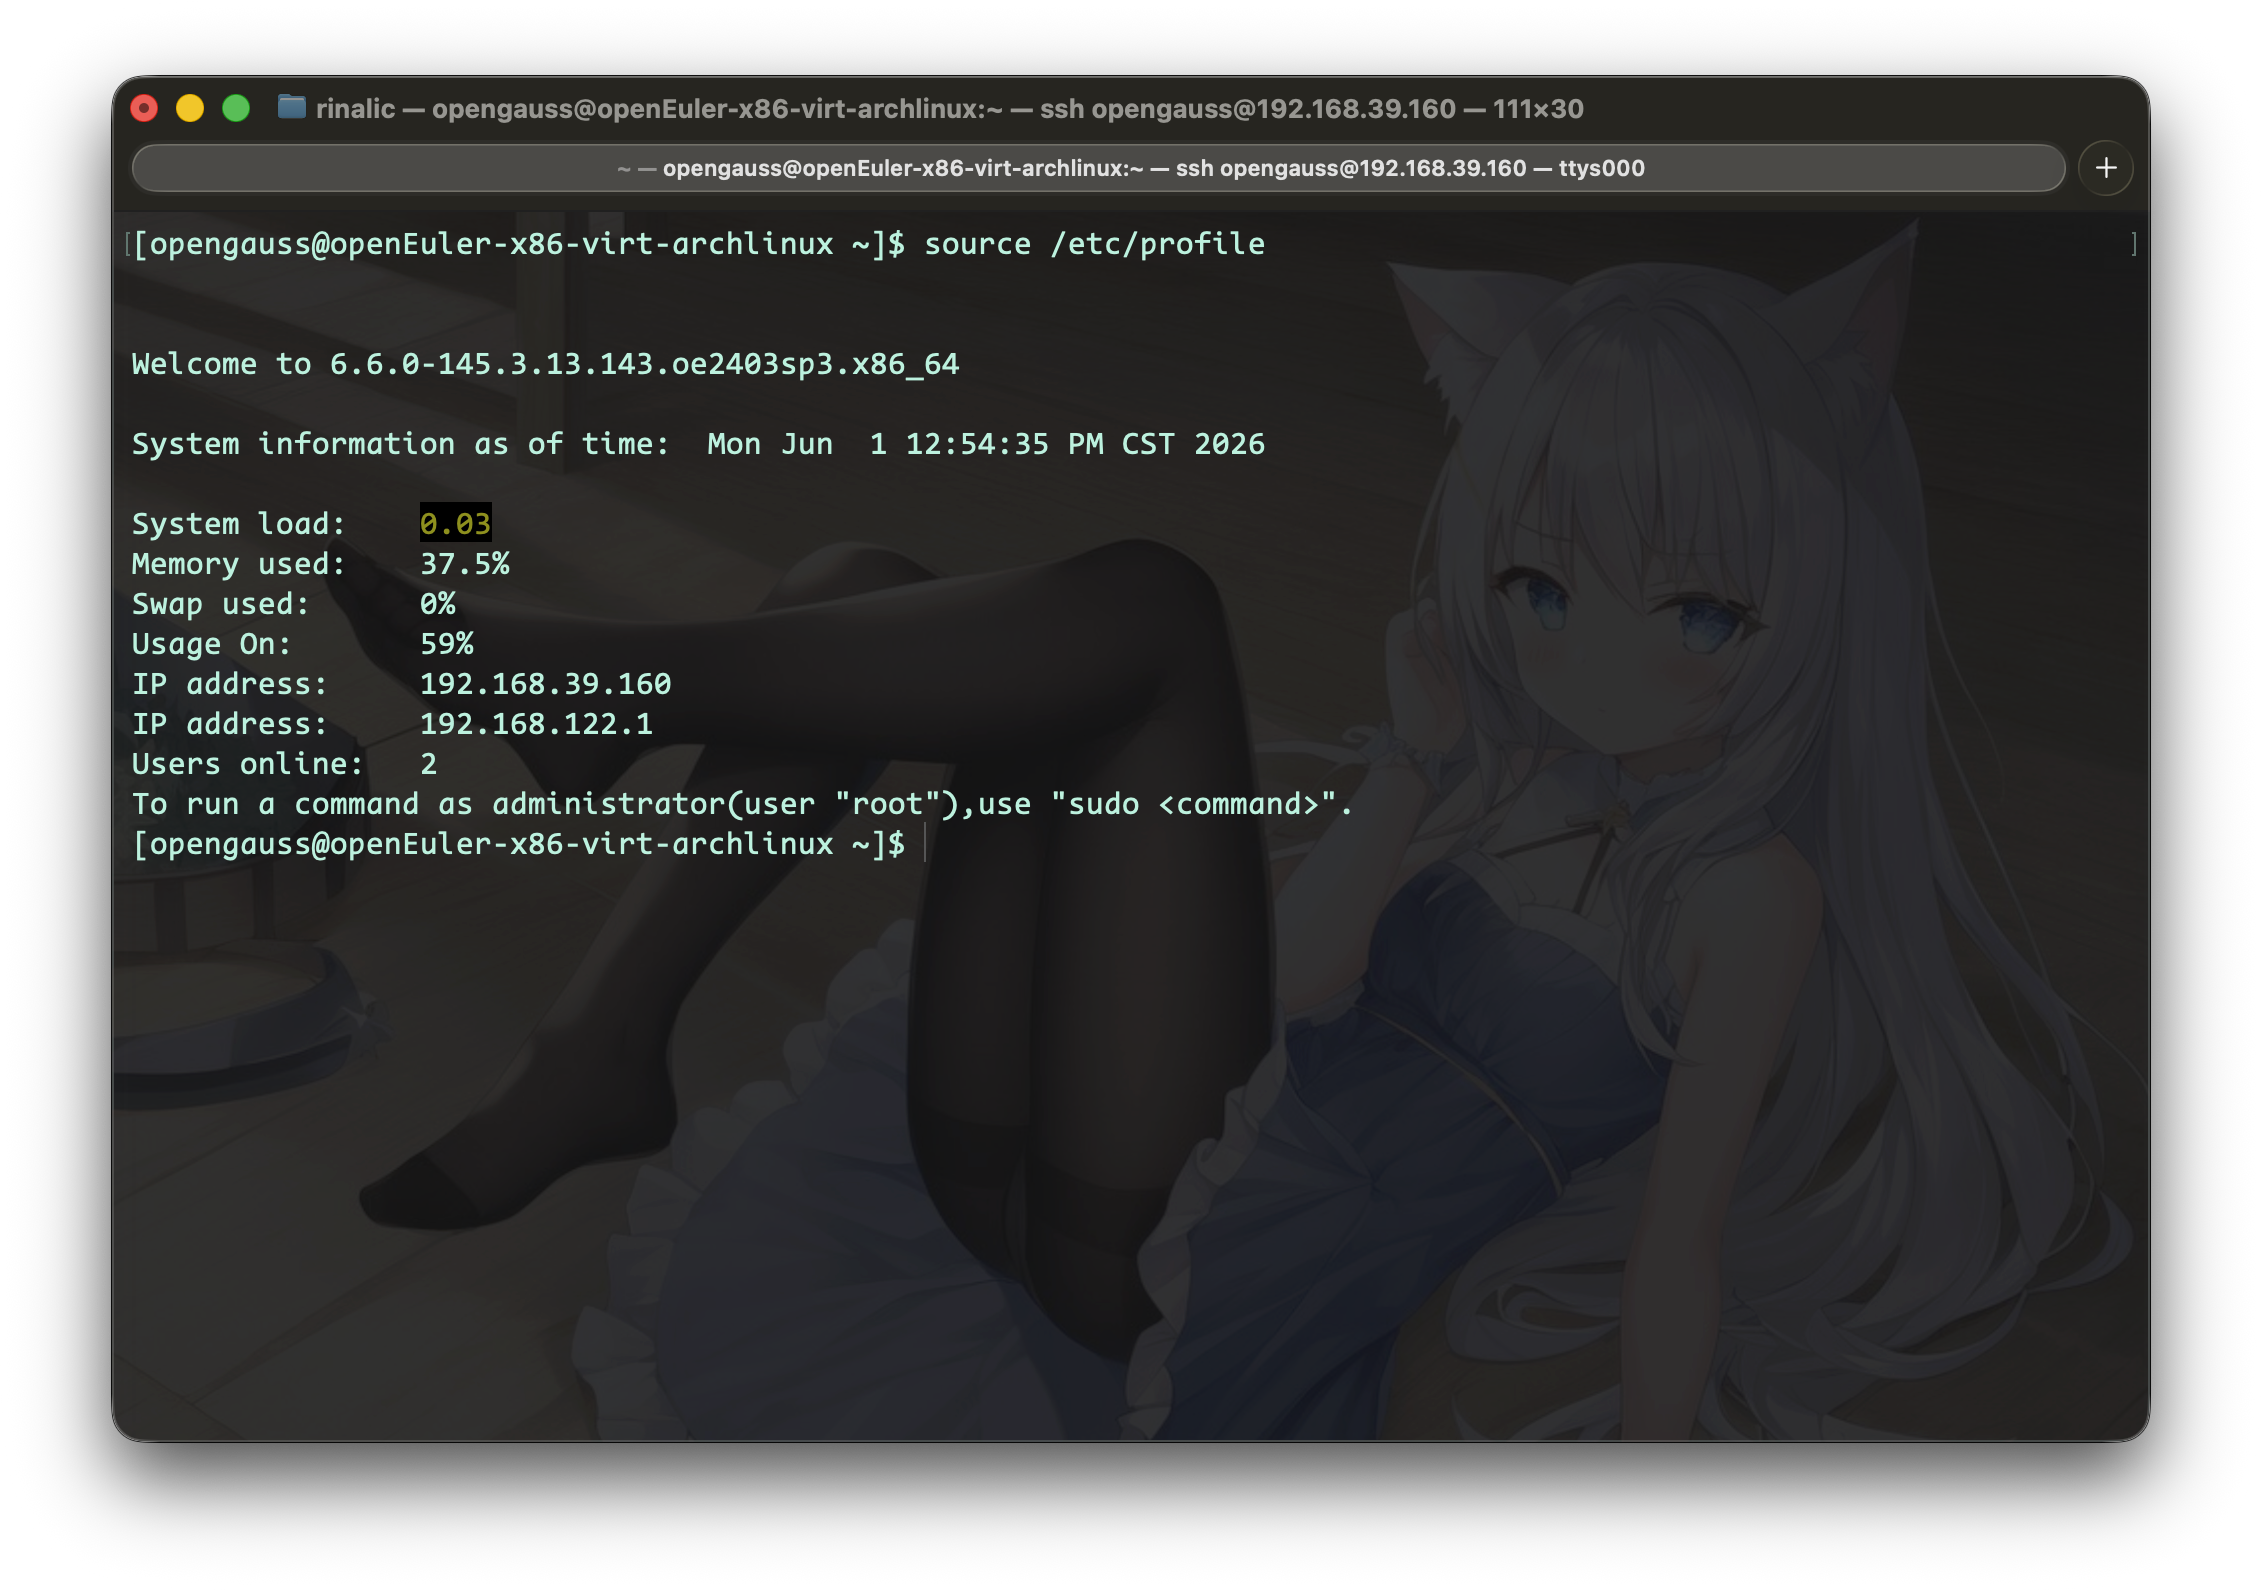
\includegraphics[width=0.88\textwidth]{images/0_ssh_opengauss.png}
\caption{SSH 登录 openEuler 虚拟机（opengauss 用户），确认 openGauss 数据库服务运行状态}
\label{fig:ssh}
\end{figure}

随后，使用 Navicat Premium 在同一局域网内通过 IP 地址远程连接至 mydb 数据库，连接成功截图如下。

\begin{figure}[H]
\centering
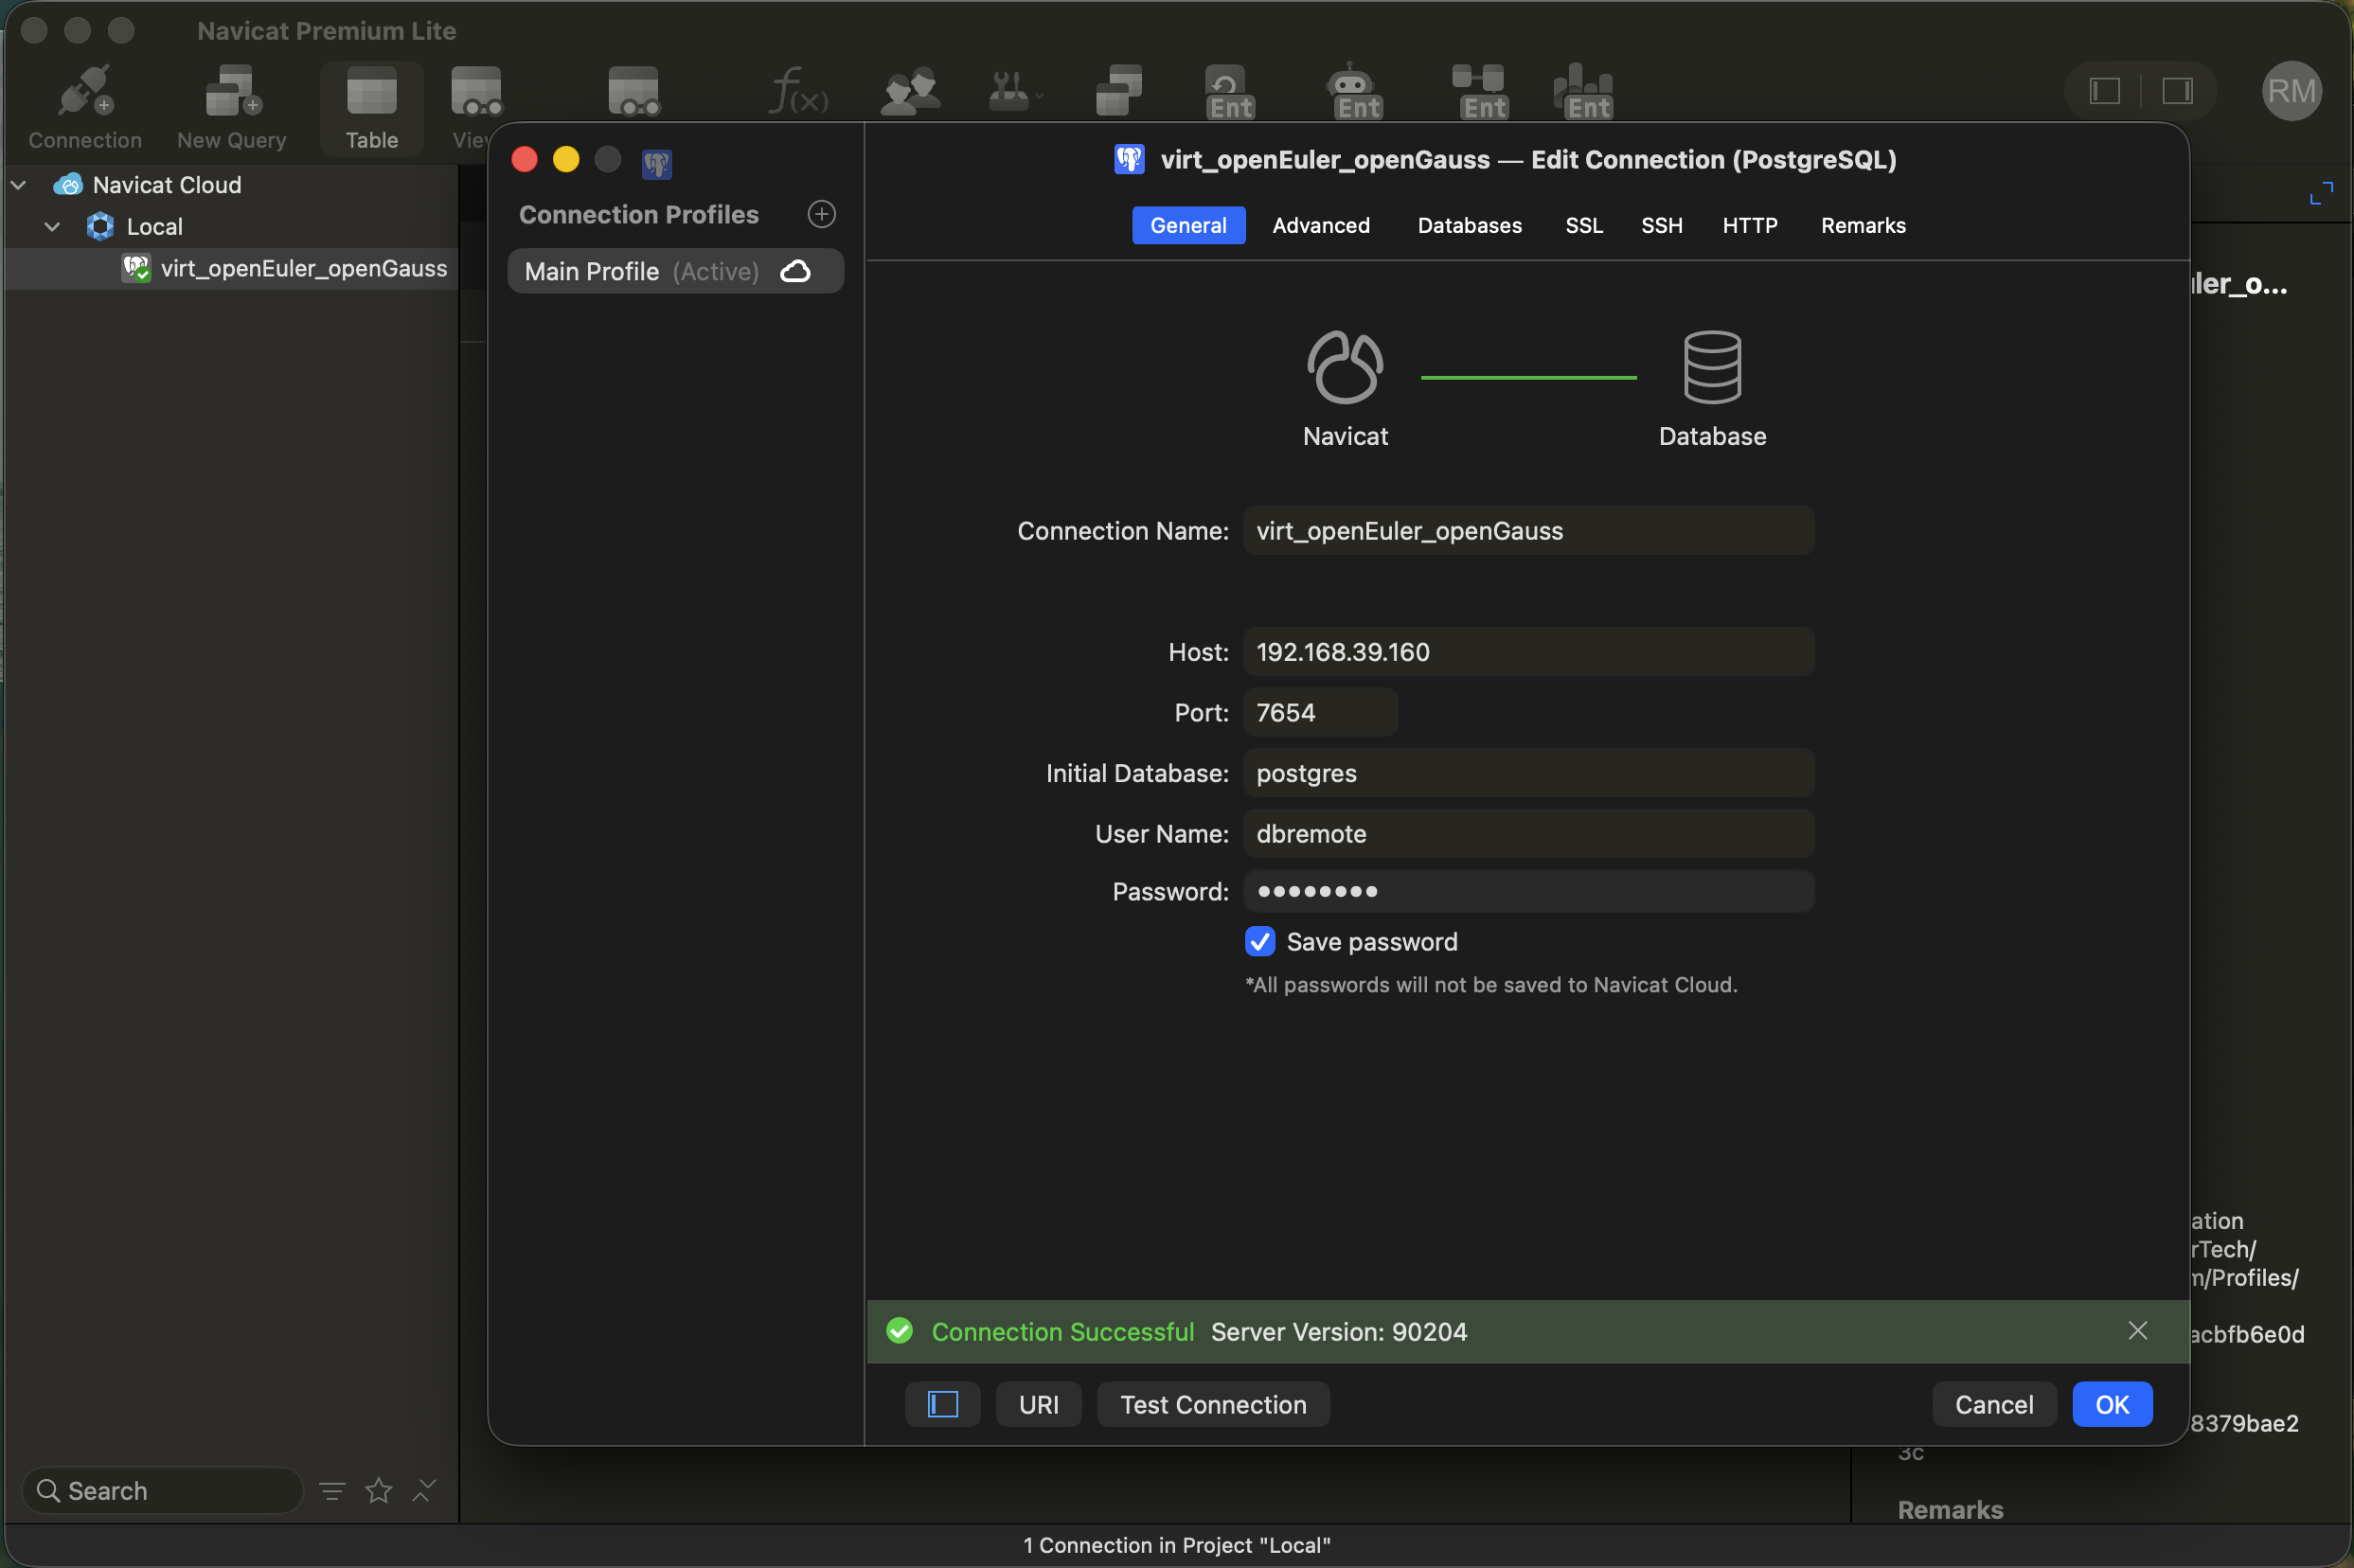
\includegraphics[width=0.85\textwidth]{images/1_navicat_remote_connect.png}
\caption{Navicat 成功远程连接至 openGauss 数据库（mydb），连接参数配置正确}
\label{fig:navicat_connect}
\end{figure}

% ===== 三、实验内容 =====
\section{实验内容}

\subsection{一、创建数据库与表结构}

\subsubsection{创建 mydb 数据库}

在 openGauss 命令行中执行以下语句，创建实验所用的 \texttt{mydb} 数据库，并指定所有者为 \texttt{dbremote} 用户：

\begin{lstlisting}[style=sqlstyle]
CREATE DATABASE "mydb"
WITH
  OWNER = "dbremote"
;
\end{lstlisting}

\subsubsection{设计并创建三张基本表}

按照实验要求，学号后三位为 "799"，因此三张表命名为 \textbf{S799}（学生表）、\textbf{C799}（课程表）、\textbf{SC799}（选课表）。各属性数据类型的选择依据如下：

\begin{itemize}
  \item \texttt{S\_num}（学号）、\texttt{C\_num}（课程编号）：选用 \texttt{VARCHAR}，保留字符串格式的灵活性，支持前缀查询（如 \texttt{LIKE 'CS\%'}）。
  \item \texttt{SNAME}、\texttt{CNAME}、\texttt{TEACHER}、\texttt{DORM}：选用 \texttt{VARCHAR}，长度按实际数据的最大估计值设置。
  \item \texttt{SEX}：选用 \texttt{VARCHAR(10)}，存储"男"或"女"。
  \item \texttt{BDATE}（出生日期）：选用 \texttt{DATE} 类型，支持日期范围查询（如 \texttt{BETWEEN}）。
  \item \texttt{HEIGHT}（身高）：选用 \texttt{DECIMAL(3,2)}，精确存储两位小数（如 1.72）。
  \item \texttt{PERIOD}（学时）：选用 \texttt{INT}，学时为整数。
  \item \texttt{CREDIT}（学分）：选用 \texttt{DECIMAL(3,1)}，保留一位小数以兼容半学分情形。
  \item \texttt{GRADE}（成绩）：选用 \texttt{DECIMAL(4,1)}，支持一位小数精度（如 91.5），且允许为 \texttt{NULL}（表示尚未录入成绩）。
\end{itemize}

建表 SQL 语句如下：

\begin{lstlisting}[style=sqlstyle]
CREATE TABLE "public"."S799" (
  "S_num"  VARCHAR(20)   NOT NULL,
  "SNAME"  VARCHAR(50)   NOT NULL,
  "SEX"    VARCHAR(10),
  "BDATE"  DATE,
  "HEIGHT" DECIMAL(3,2),
  "DORM"   VARCHAR(100),
  PRIMARY KEY ("S_num")
);

CREATE TABLE "public"."C799" (
  "C_num"   VARCHAR(20)  NOT NULL,
  "CNAME"   VARCHAR(100) NOT NULL,
  "PERIOD"  INT,
  "CREDIT"  DECIMAL(3,1),
  "TEACHER" VARCHAR(50),
  PRIMARY KEY ("C_num")
);

CREATE TABLE "public"."SC799" (
  "S_num"  VARCHAR(20),
  "C_num"  VARCHAR(20),
  "GRADE"  DECIMAL(4,1),
  PRIMARY KEY ("S_num", "C_num"),
  FOREIGN KEY ("S_num") REFERENCES "S799"("S_num"),
  FOREIGN KEY ("C_num") REFERENCES "C799"("C_num")
);
\end{lstlisting}

SC799 表以 (\texttt{S\_num}, \texttt{C\_num}) 构成联合主键，同时对两字段分别设置外键约束，引用 S799 和 C799 的主键，保证参照完整性——禁止插入不存在的学号或课程编号对应的选课记录。

\begin{figure}[H]
\centering
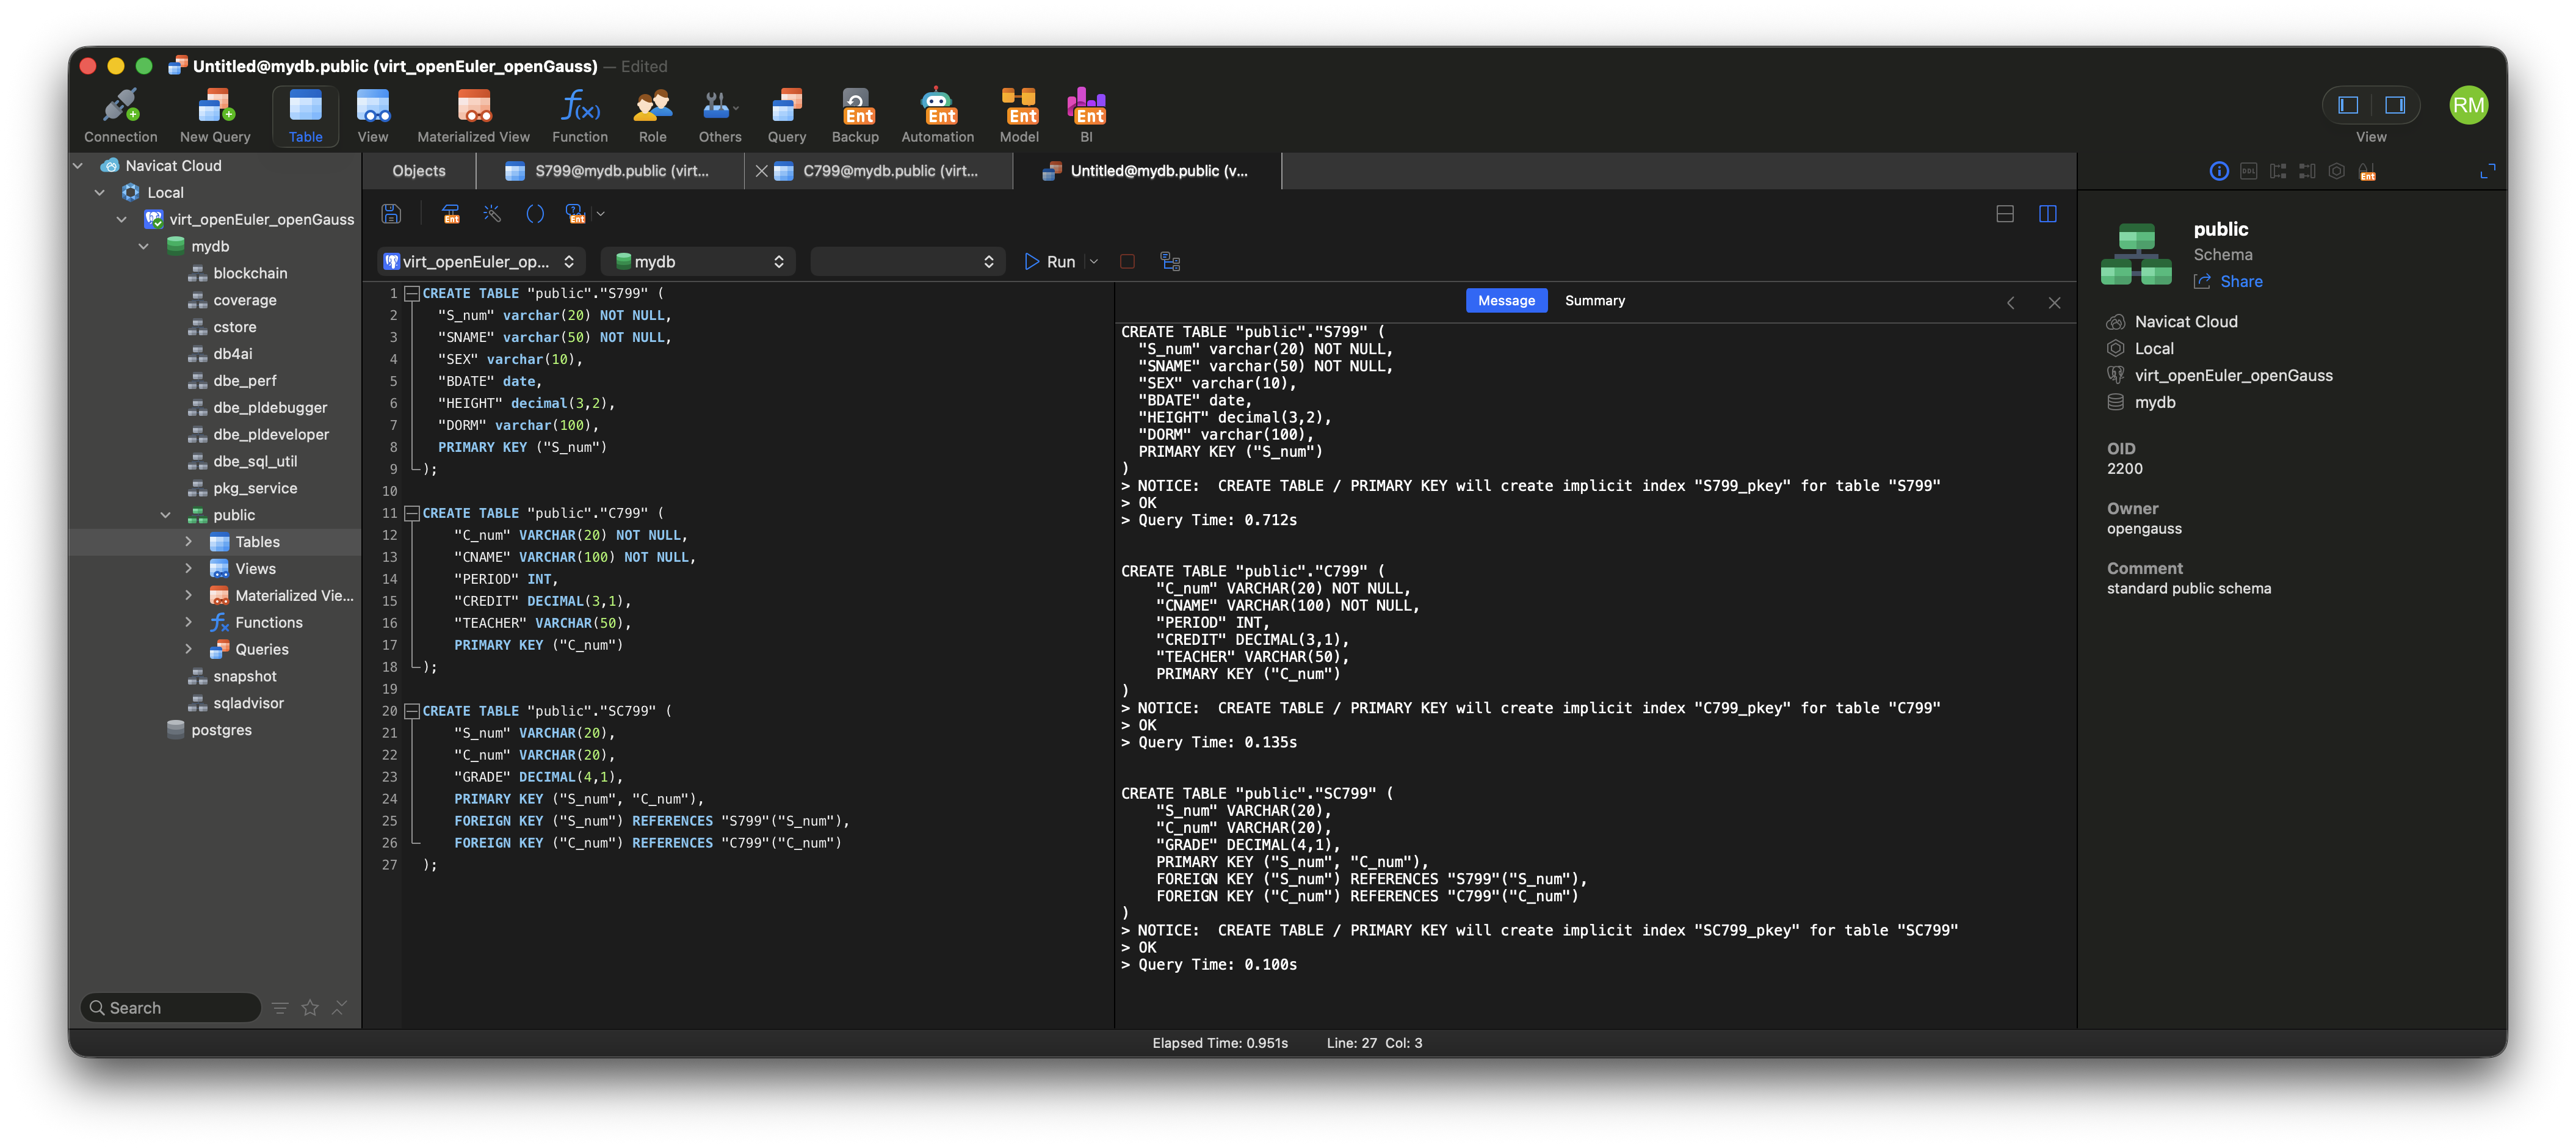
\includegraphics[width=0.90\textwidth]{images/2_create_tables.png}
\caption{在 Navicat 查询编辑器中执行建表 SQL，成功创建 S799、C799、SC799 三张表}
\label{fig:create_tables}
\end{figure}

\subsection{二、数据录入与属性查询}

\subsubsection{向各表插入初始数据}

按照实验题目给定的数据，依次向三张表插入记录。

\paragraph{插入学生表 S799}

共插入 11 条学生记录，涵盖不同性别、出生年份和宿舍楼栋：

\begin{lstlisting}[style=sqlstyle]
INSERT INTO "public"."S799"
  ("S_num","SNAME","SEX","BDATE","HEIGHT","DORM")
VALUES
  ('01032010','王涛',  '男','2004-04-05',1.72,'东6舍221'),
  ('01032023','孙文',  '男','2005-06-10',1.80,'东6舍221'),
  ('01032001','张晓梅','女','2004-11-17',1.58,'东1舍312'),
  ('01032005','刘静',  '女','2004-01-10',1.63,'东1舍312'),
  ('01032112','许澍',  '男','2004-02-20',1.71,'东6舍221'),
  ('03031011','王倩',  '女','2005-09-20',1.66,'东2舍104'),
  ('03031014','赵思扬','男','2003-06-06',1.85,'东18舍421'),
  ('03031051','周剑',  '男','2003-05-08',1.68,'东18舍422'),
  ('03031009','田菲',  '女','2004-08-11',1.60,'东2舍104'),
  ('03031033','蔡明明','男','2004-03-12',1.75,'东18舍423'),
  ('03031056','曹子衿','女','2006-12-15',1.65,'东2舍305');
\end{lstlisting}

\begin{figure}[H]
\centering
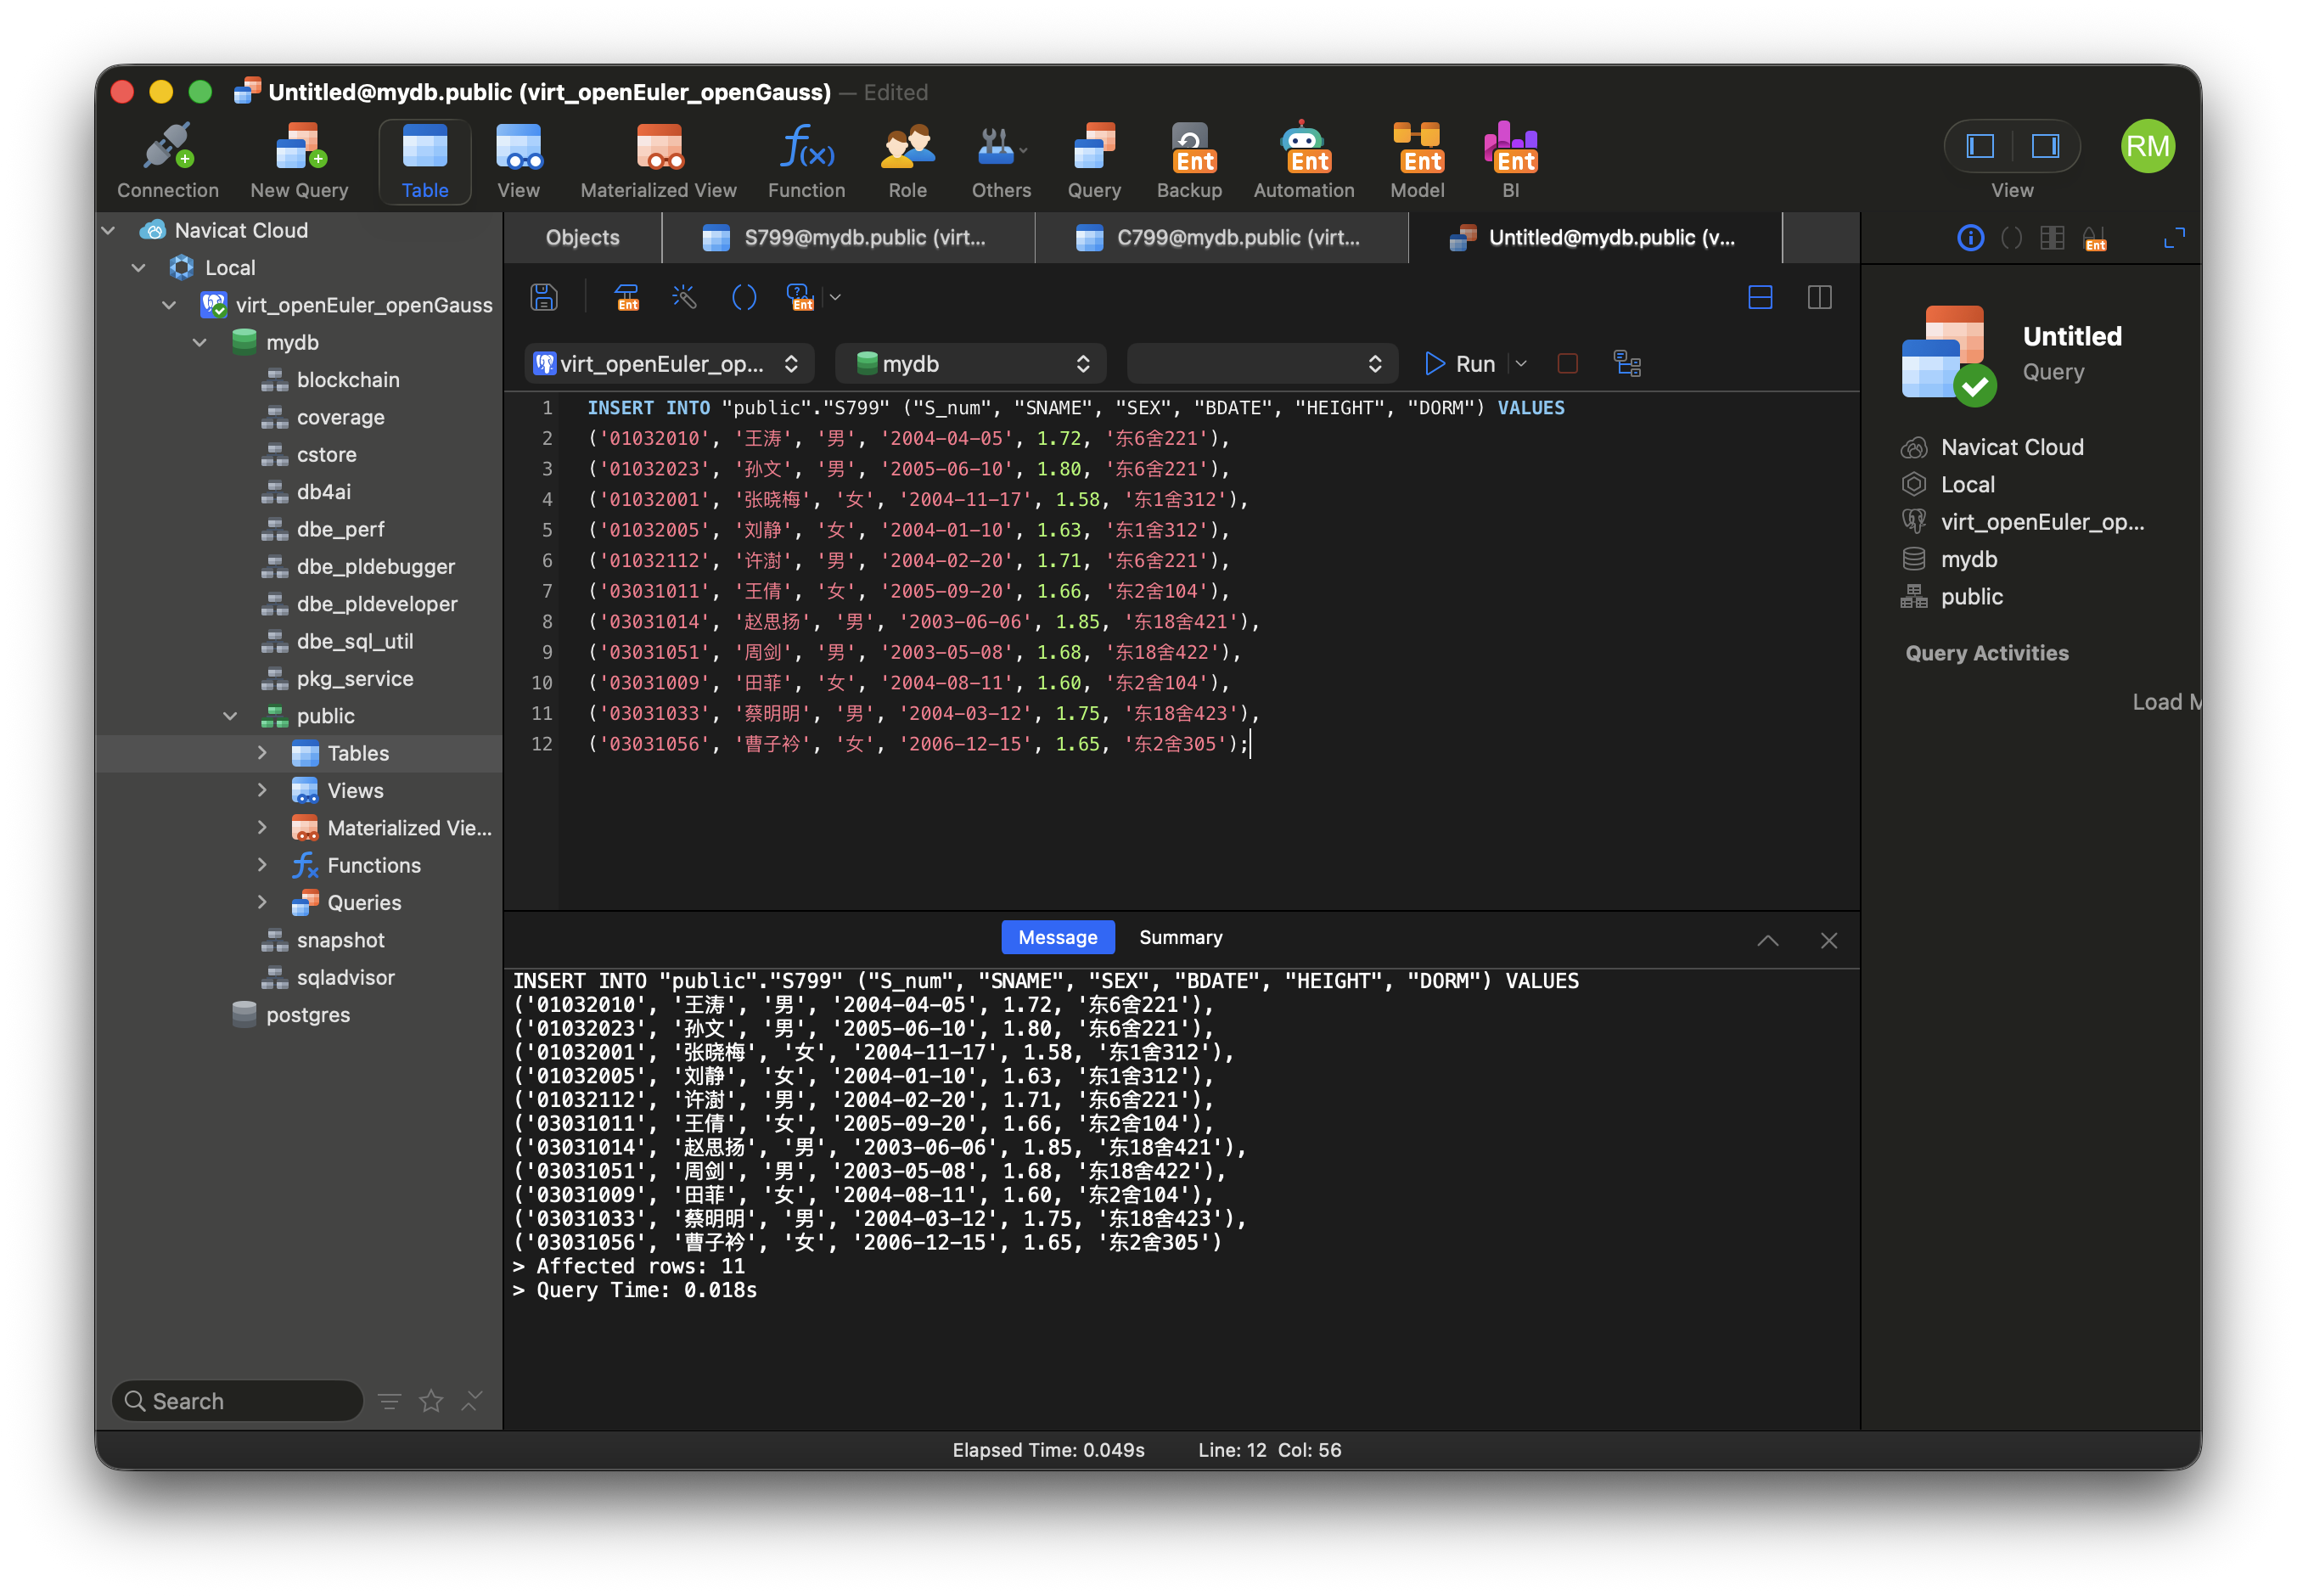
\includegraphics[width=0.90\textwidth]{images/3_insert_s799.png}
\caption{向 S799 表插入 11 条学生记录，执行成功}
\label{fig:insert_s799}
\end{figure}

\paragraph{插入课程表 C799}

共插入 7 门课程，分属计算机系（CS 前缀）和电子系（EE 前缀）两个系别：

\begin{lstlisting}[style=sqlstyle]
INSERT INTO "public"."C799"
  ("C_num","CNAME","PERIOD","CREDIT","TEACHER")
VALUES
  ('CS-01','数据结构',        60,3,'张军'),
  ('CS-02','计算机组成原理',  80,4,'王亚伟'),
  ('CS-04','人工智能',        40,2,'李蕾'),
  ('CS-05','深度学习',        40,2,'崔昀'),
  ('EE-01','信号与系统',      60,3,'张明'),
  ('EE-02','数字逻辑电路',   100,5,'胡海东'),
  ('EE-03','光电子学与光子学',40,2,'石韬');
\end{lstlisting}

\begin{figure}[H]
\centering
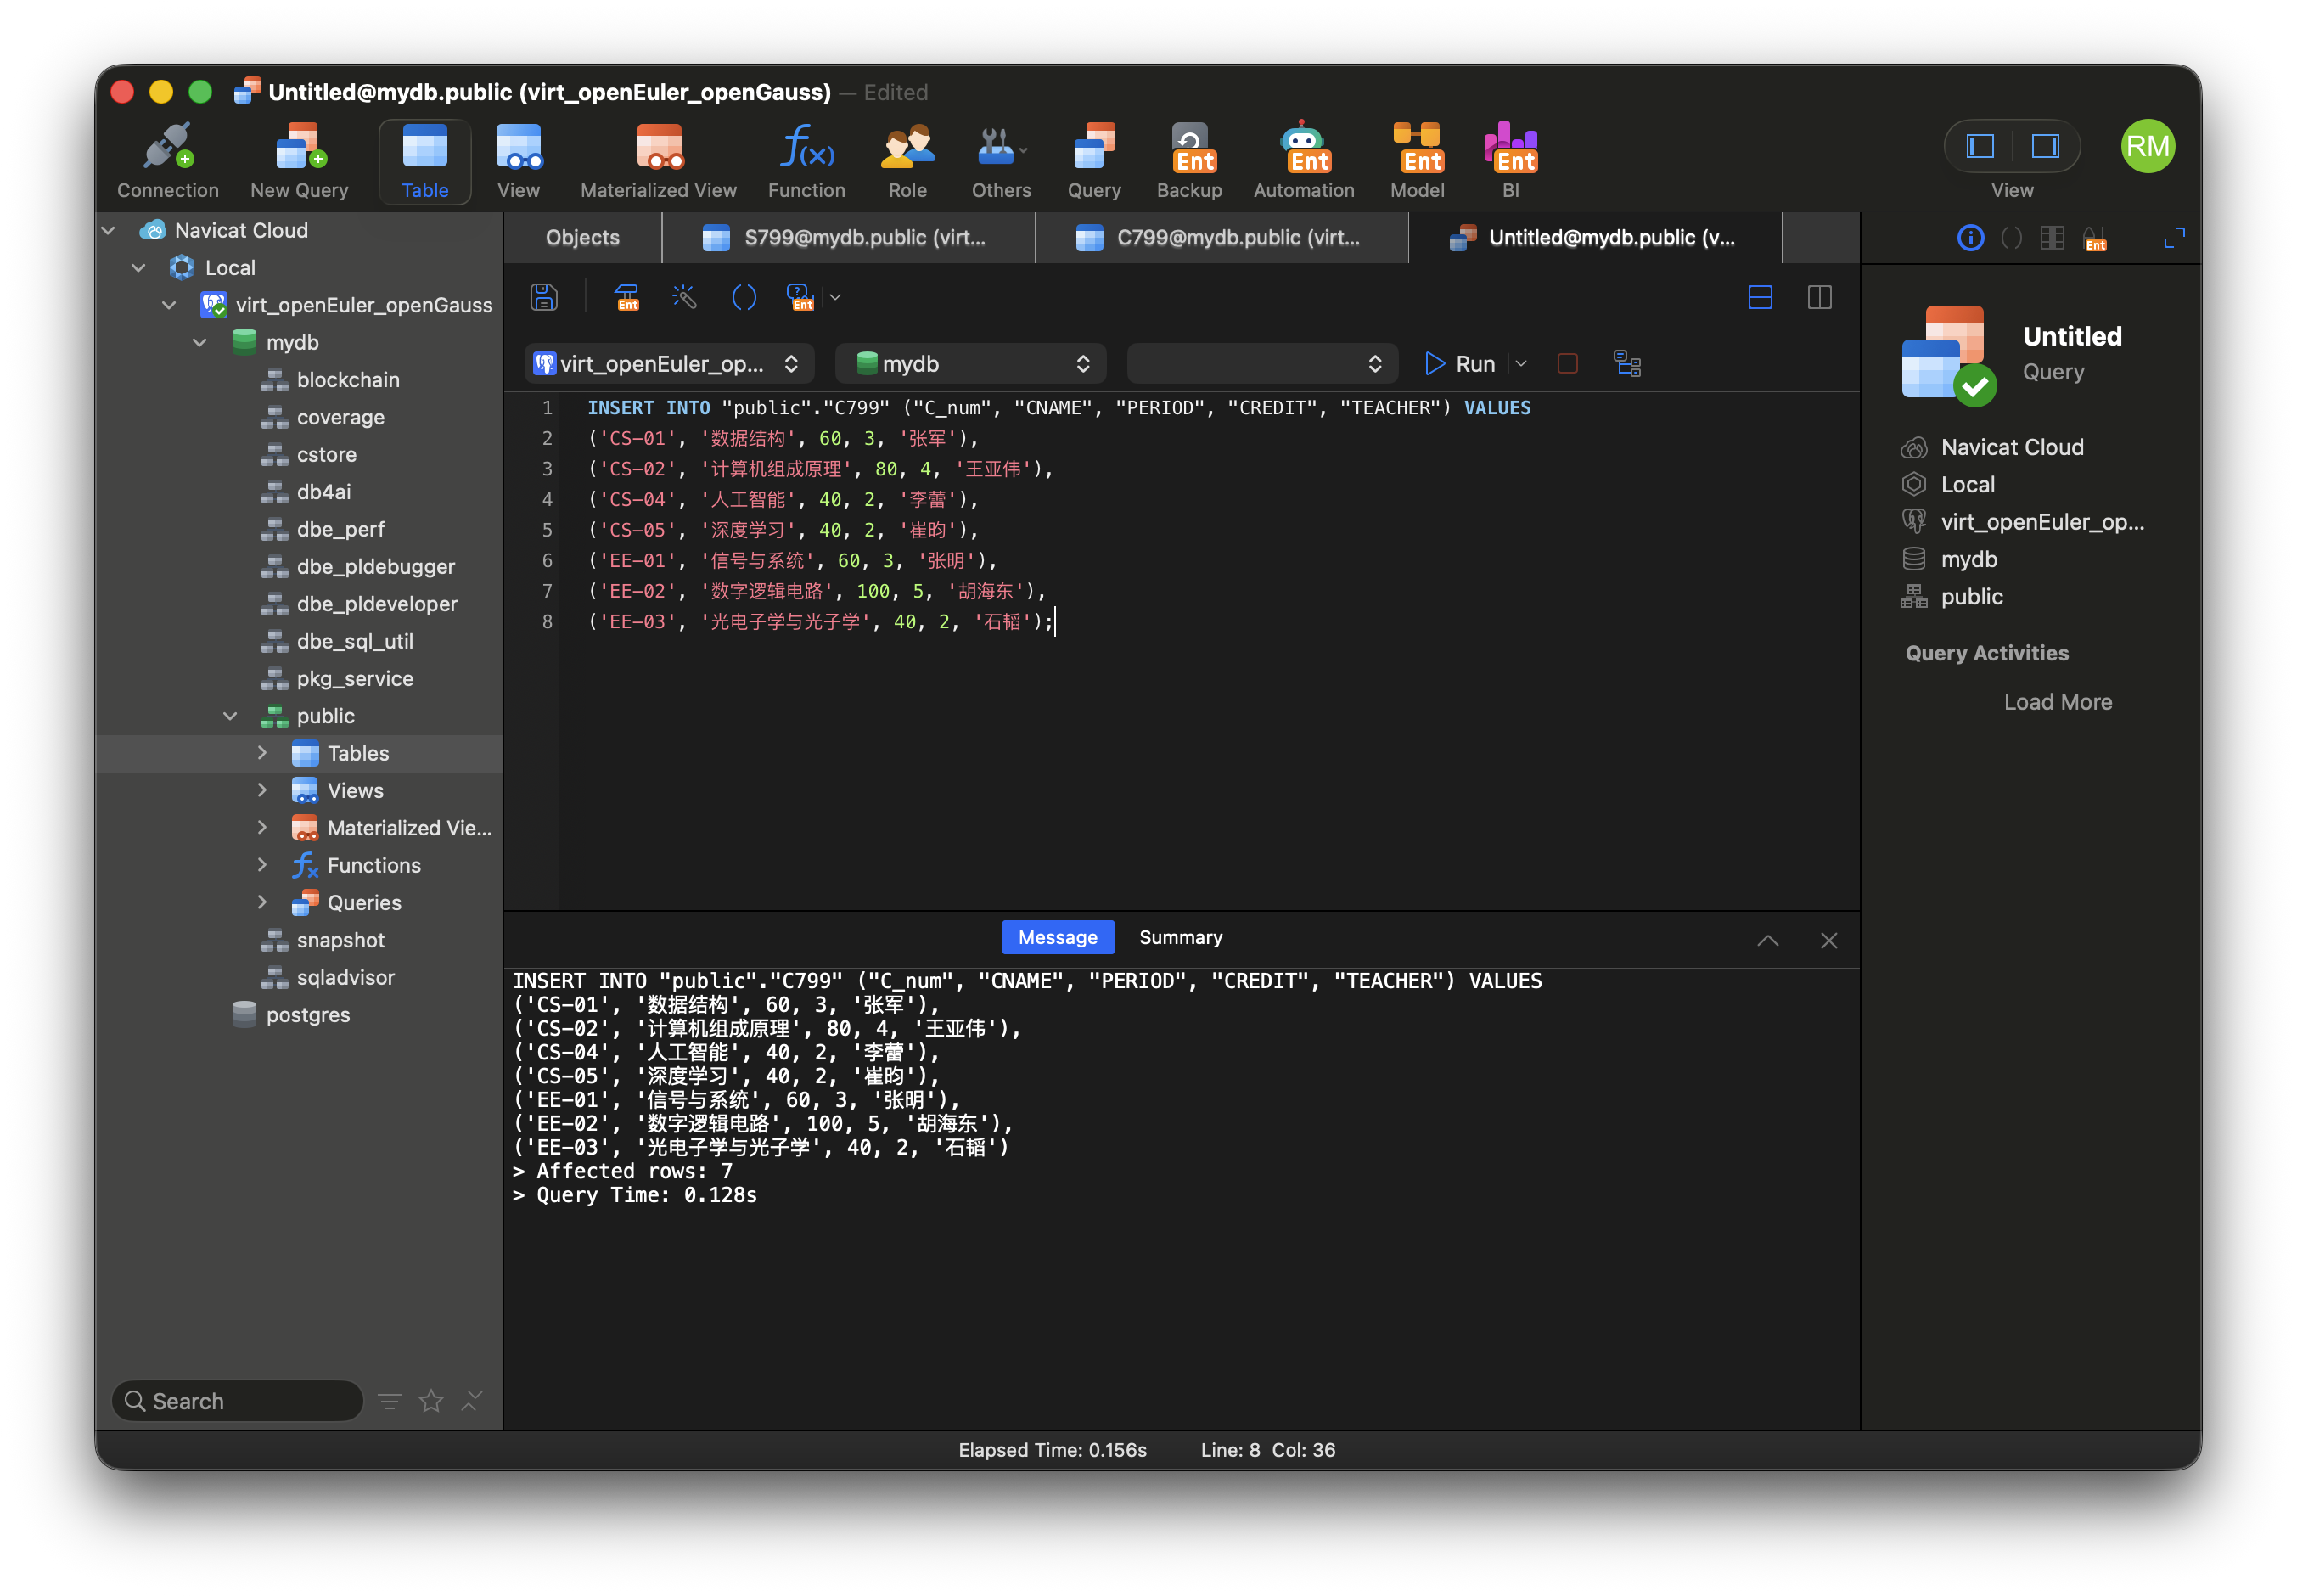
\includegraphics[width=0.90\textwidth]{images/4_insert_c799.png}
\caption{向 C799 表插入 7 条课程记录，执行成功}
\label{fig:insert_c799}
\end{figure}

\paragraph{插入选课表 SC799}

共插入 26 条选课记录。其中许澍（\texttt{01032112}）选修深度学习（\texttt{CS-05}）尚无成绩，对应成绩字段插入 \texttt{NULL}：

\begin{lstlisting}[style=sqlstyle]
INSERT INTO "public"."SC799" ("S_num","C_num","GRADE")
VALUES
  ('01032010','CS-01',82.0), ('01032010','CS-02',91.0),
  ('01032010','CS-04',83.5), ('01032001','CS-01',77.5),
  ('01032001','CS-02',85.0), ('01032001','CS-04',83.0),
  ('01032005','CS-01',62.0), ('01032005','CS-02',77.0),
  ('01032005','CS-04',82.0), ('01032023','CS-01',55.0),
  ('01032023','CS-02',81.0), ('01032023','CS-04',76.0),
  ('01032112','CS-01',88.0), ('01032112','CS-02',91.5),
  ('01032112','CS-04',86.0), ('01032112','CS-05',NULL),
  ('03031033','EE-01',93.0), ('03031033','EE-02',89.0),
  ('03031009','EE-01',88.0), ('03031009','EE-02',78.5),
  ('03031011','EE-01',91.0), ('03031011','EE-02',86.0),
  ('03031051','EE-01',78.0), ('03031051','EE-02',58.0),
  ('03031014','EE-01',79.0), ('03031014','EE-02',71.0);
\end{lstlisting}

\begin{figure}[H]
\centering
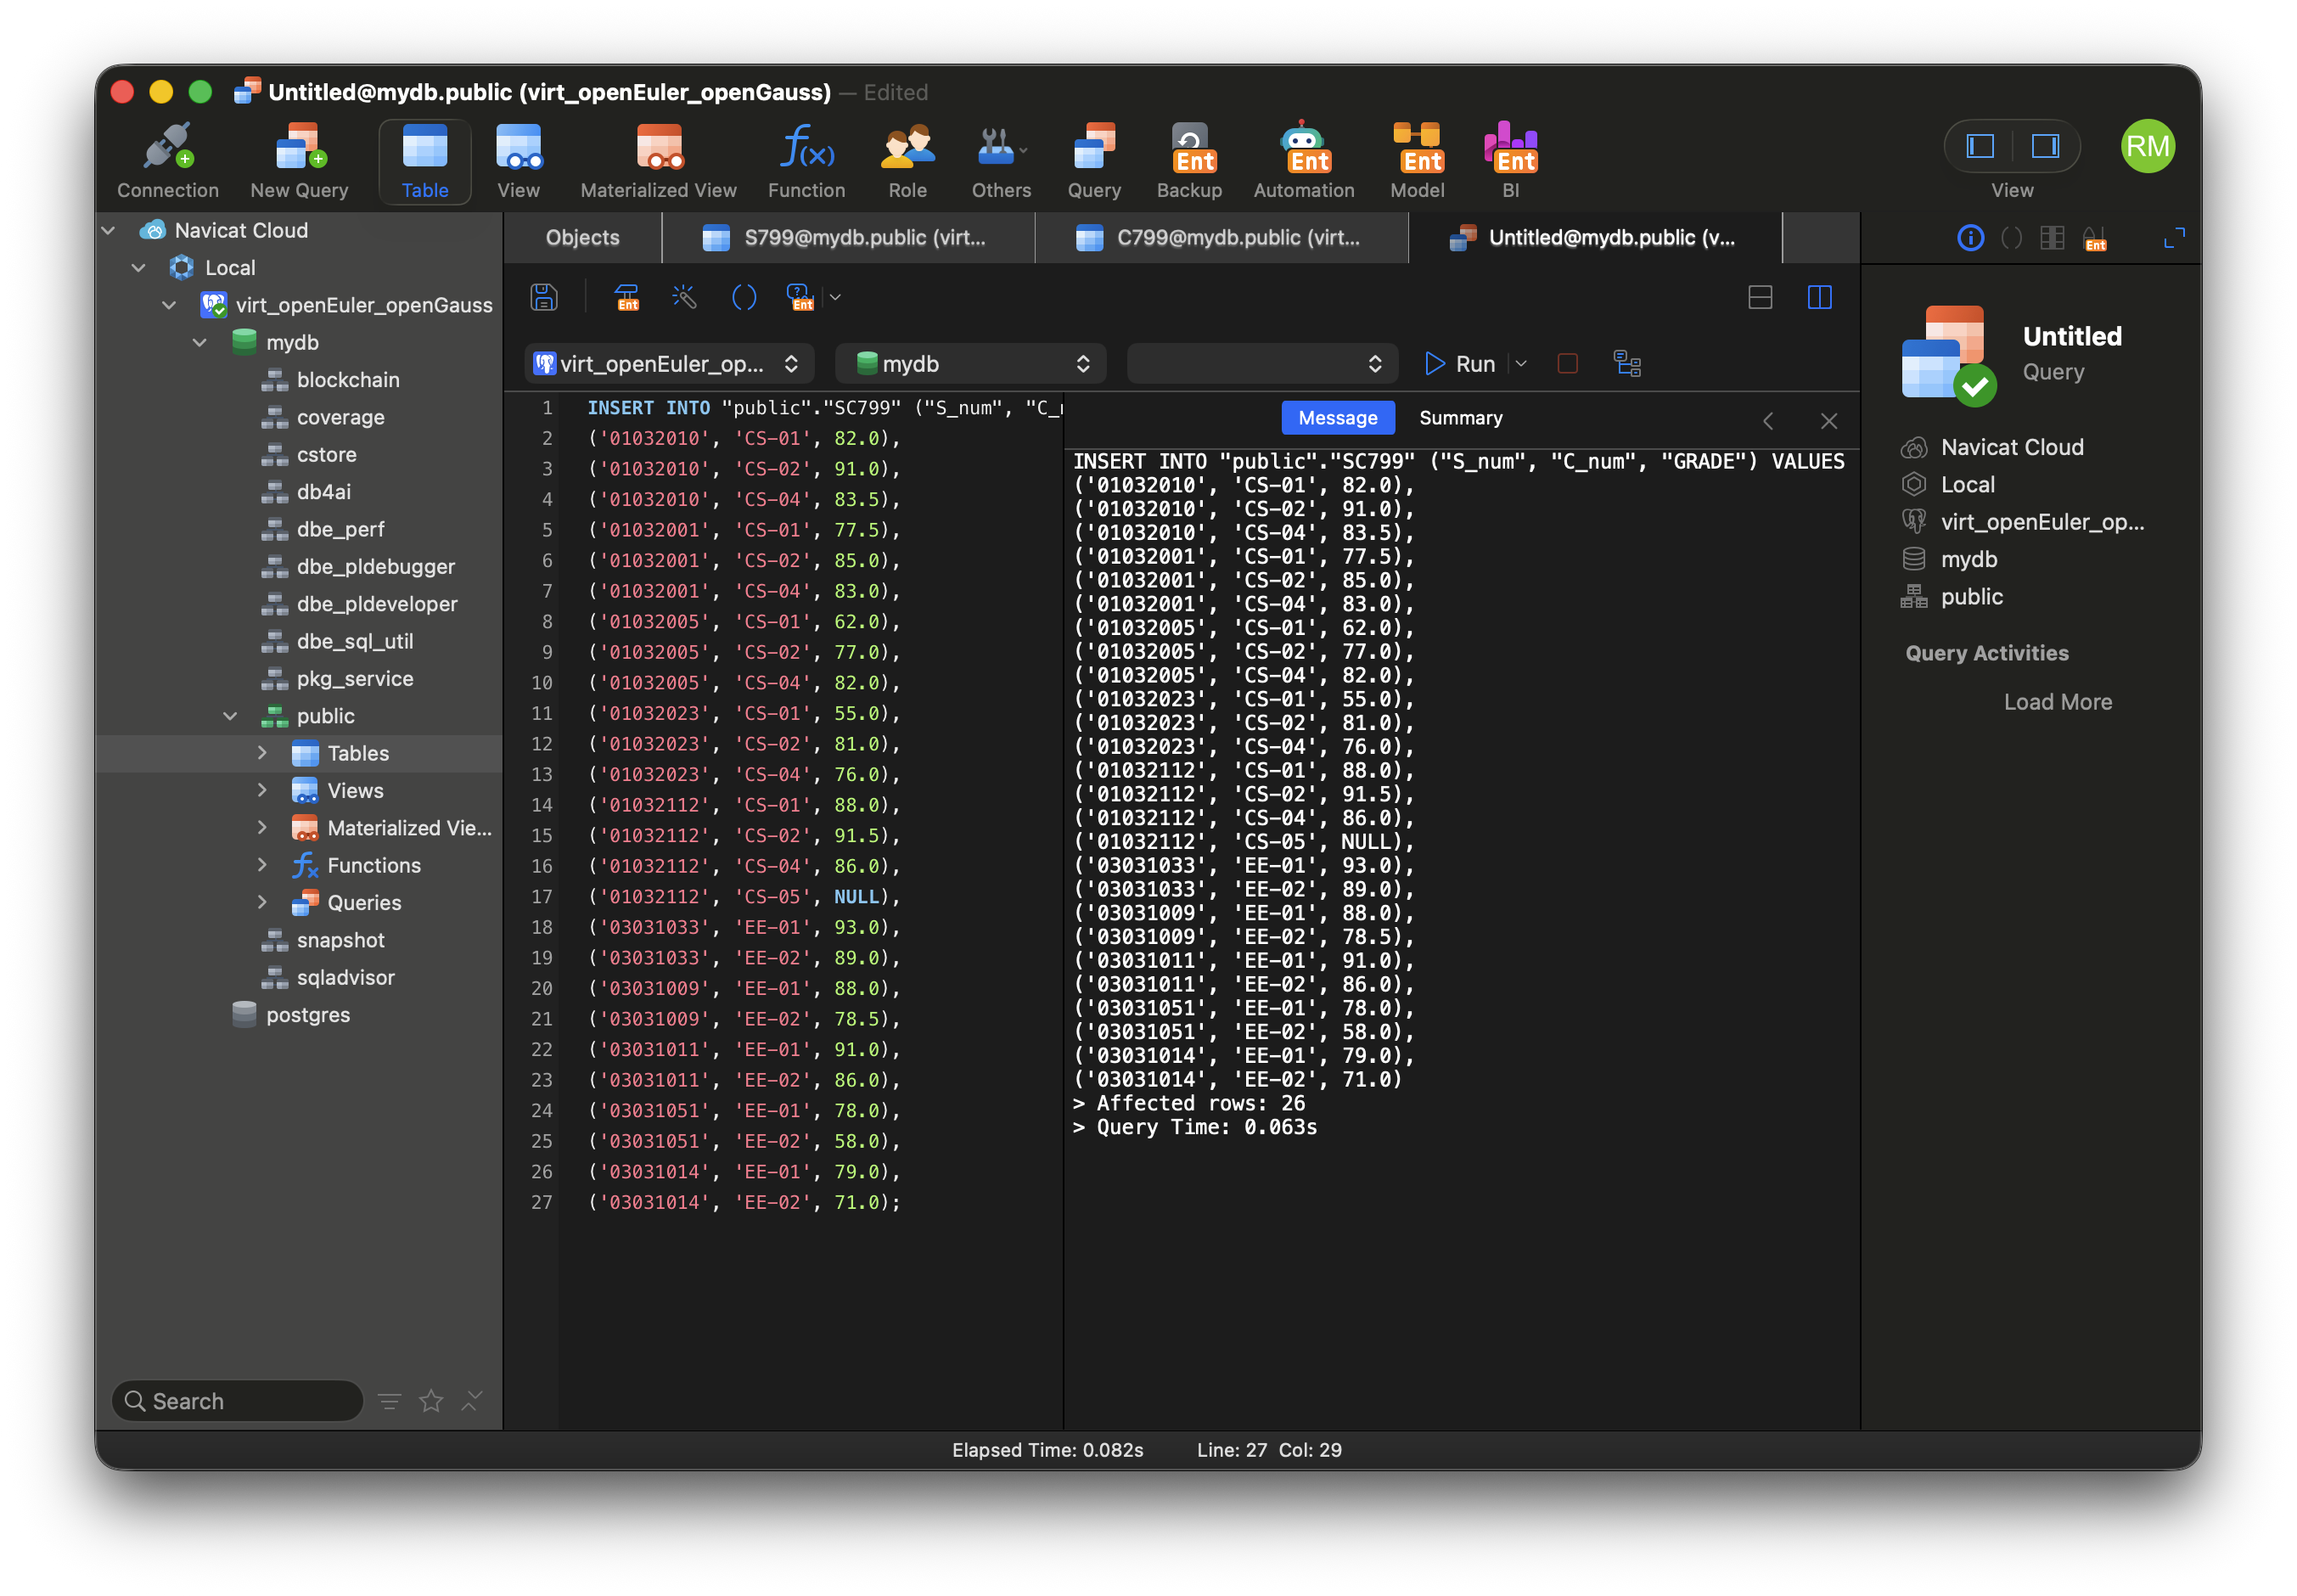
\includegraphics[width=0.90\textwidth]{images/5_insert_sc799.png}
\caption{向 SC799 表插入 26 条选课记录（含 1 条 NULL 成绩），执行成功}
\label{fig:insert_sc799}
\end{figure}

\subsubsection{查询数据目录中的表与属性信息}

通过查询 \texttt{information\_schema.columns} 系统视图，可获取三张表的元信息，包括属性名称、数据类型、最大长度及是否允许为空：

\begin{lstlisting}[style=sqlstyle]
SELECT
    table_name              AS "表名",
    column_name             AS "属性名",
    data_type               AS "数据类型",
    character_maximum_length AS "最大长度",
    is_nullable             AS "是否允许为空"
FROM information_schema.columns
WHERE table_schema = 'public'
  AND table_name IN ('S799','C799','SC799')
ORDER BY table_name, ordinal_position;
\end{lstlisting}

\begin{figure}[H]
\centering
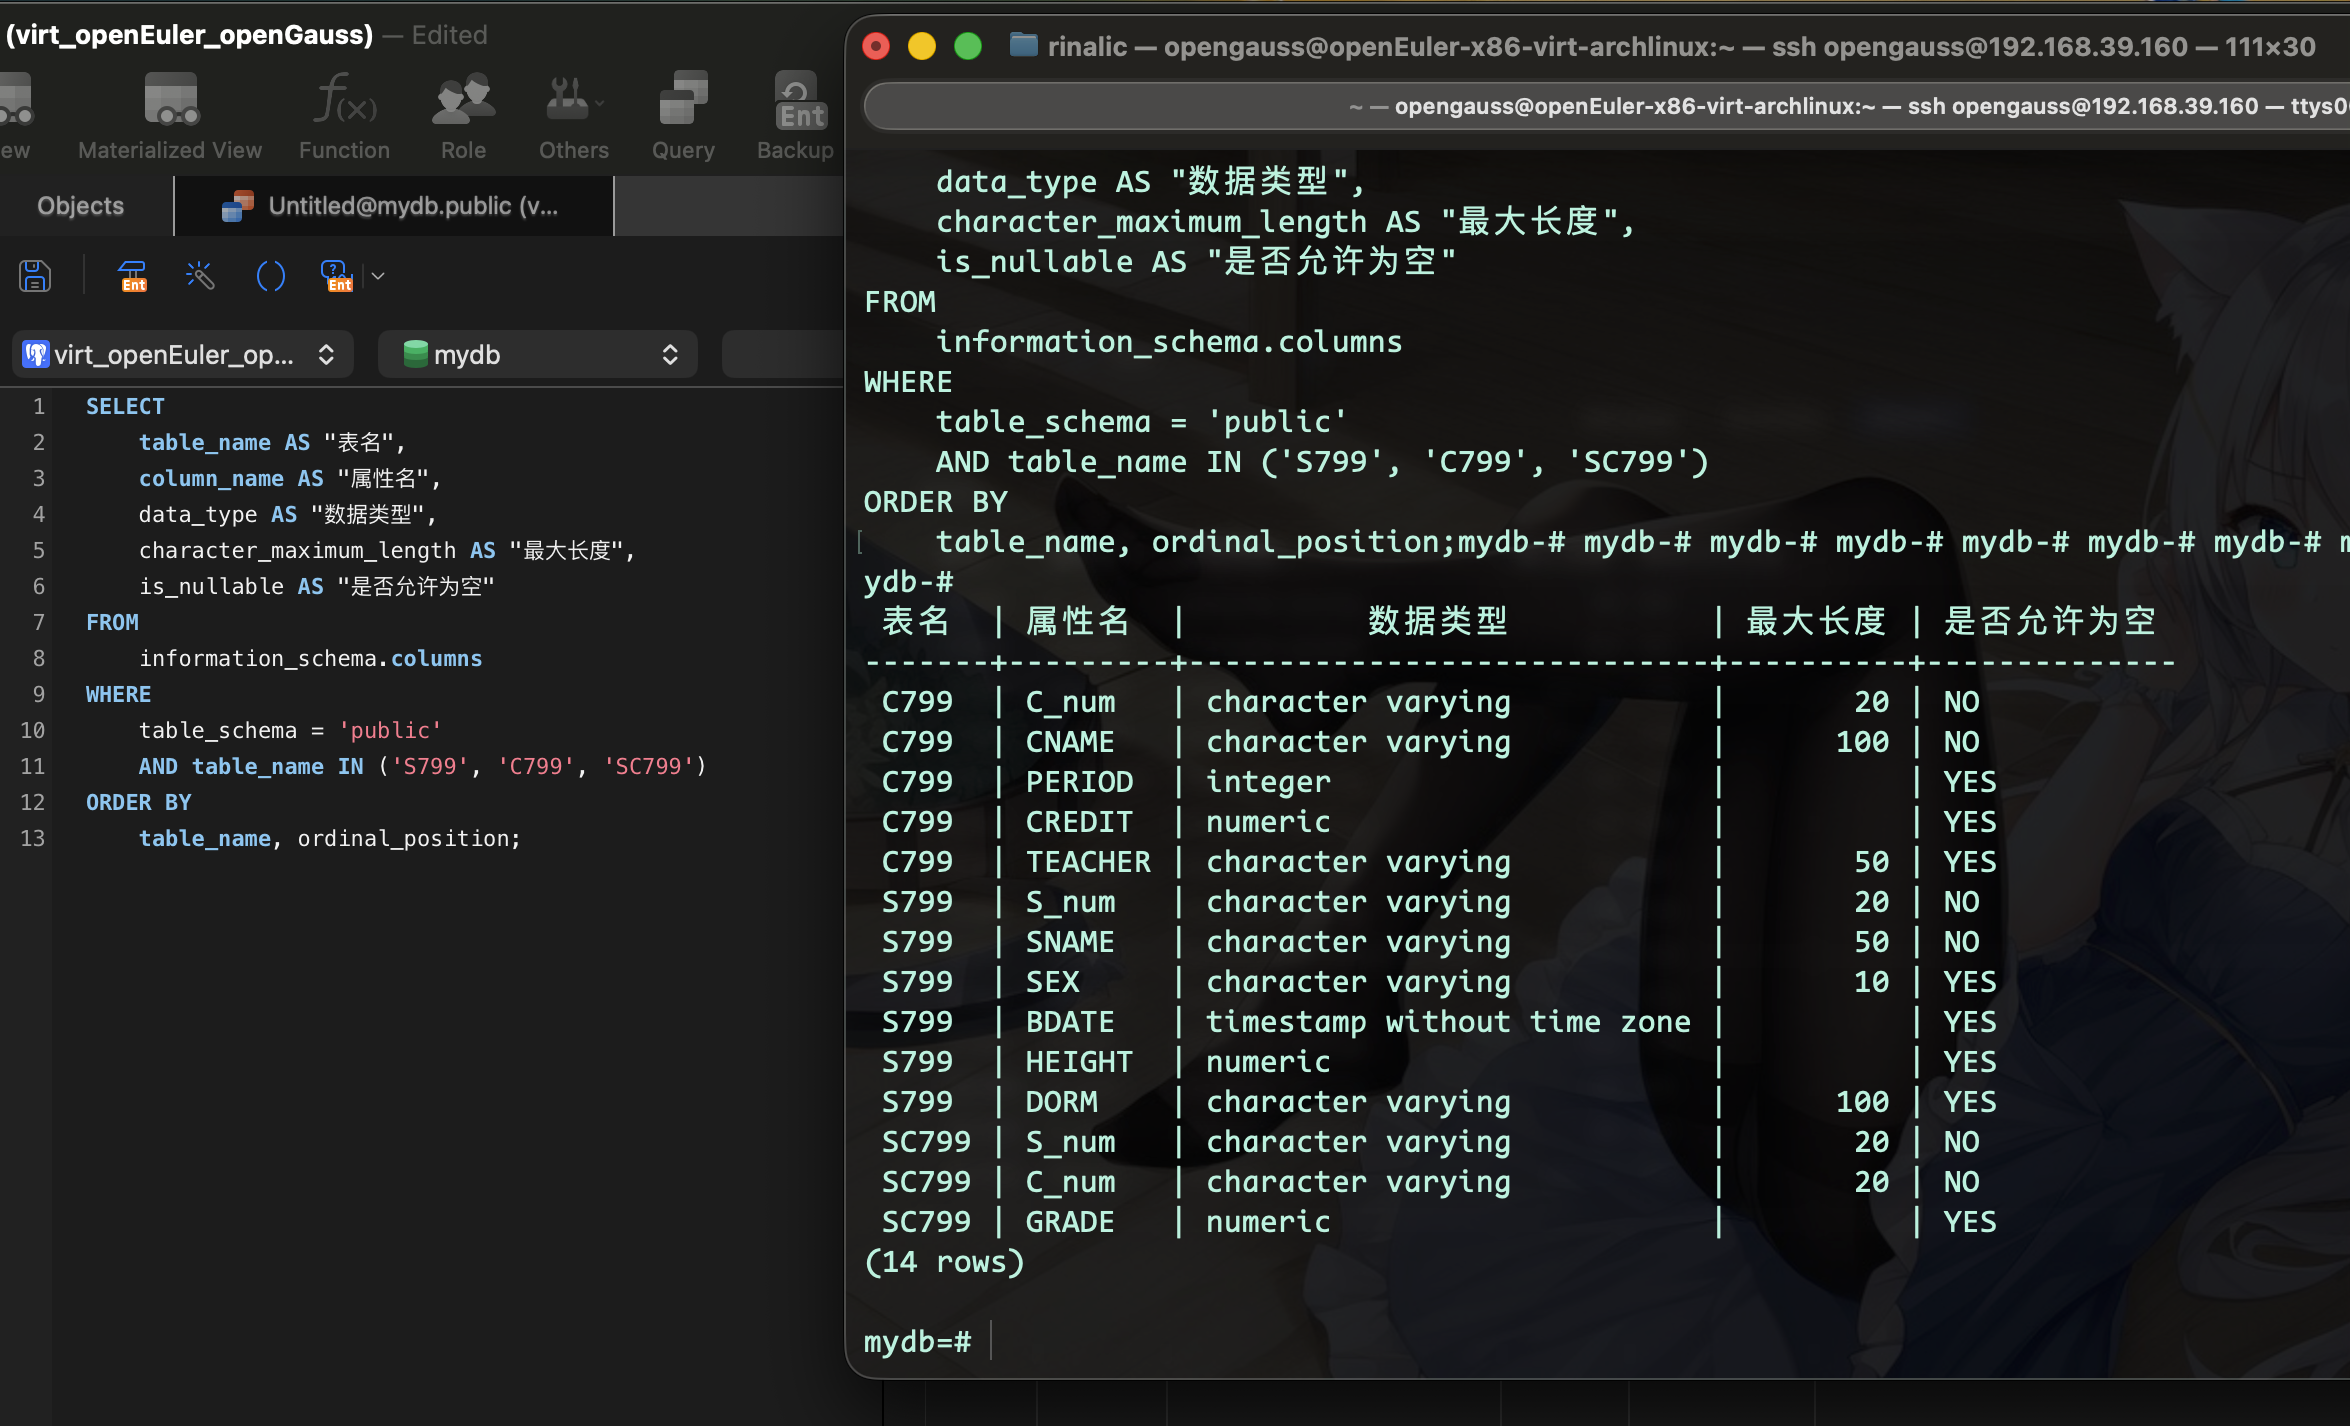
\includegraphics[width=0.90\textwidth]{images/6_query_tables_and_attributes.png}
\caption{通过系统数据目录视图查询 S799、C799、SC799 三表的全部属性信息}
\label{fig:query_attrs}
\end{figure}

查询结果清晰展示了三张表的全部属性及约束，与建表设计完全一致：S799 有 6 个属性（主键 S\_num），C799 有 5 个属性（主键 C\_num），SC799 有 3 个属性（联合主键 + 两个外键）。

\subsection{三、SQL 基本操作}

\subsubsection{1. 复杂查询}

\paragraph{(1) 查询计算机系（CS）所开课程的课程编号、课程名称及学分数}

\textbf{思路}：利用 \texttt{LIKE 'CS\%'} 对课程编号进行前缀匹配，直接从 C799 表中筛选计算机系课程，查询课程编号、名称和学分三个字段。

\begin{lstlisting}[style=sqlstyle]
SELECT "C_num", "CNAME", "CREDIT"
FROM "public"."C799"
WHERE "C_num" LIKE 'CS%';
\end{lstlisting}

\begin{figure}[H]
\centering
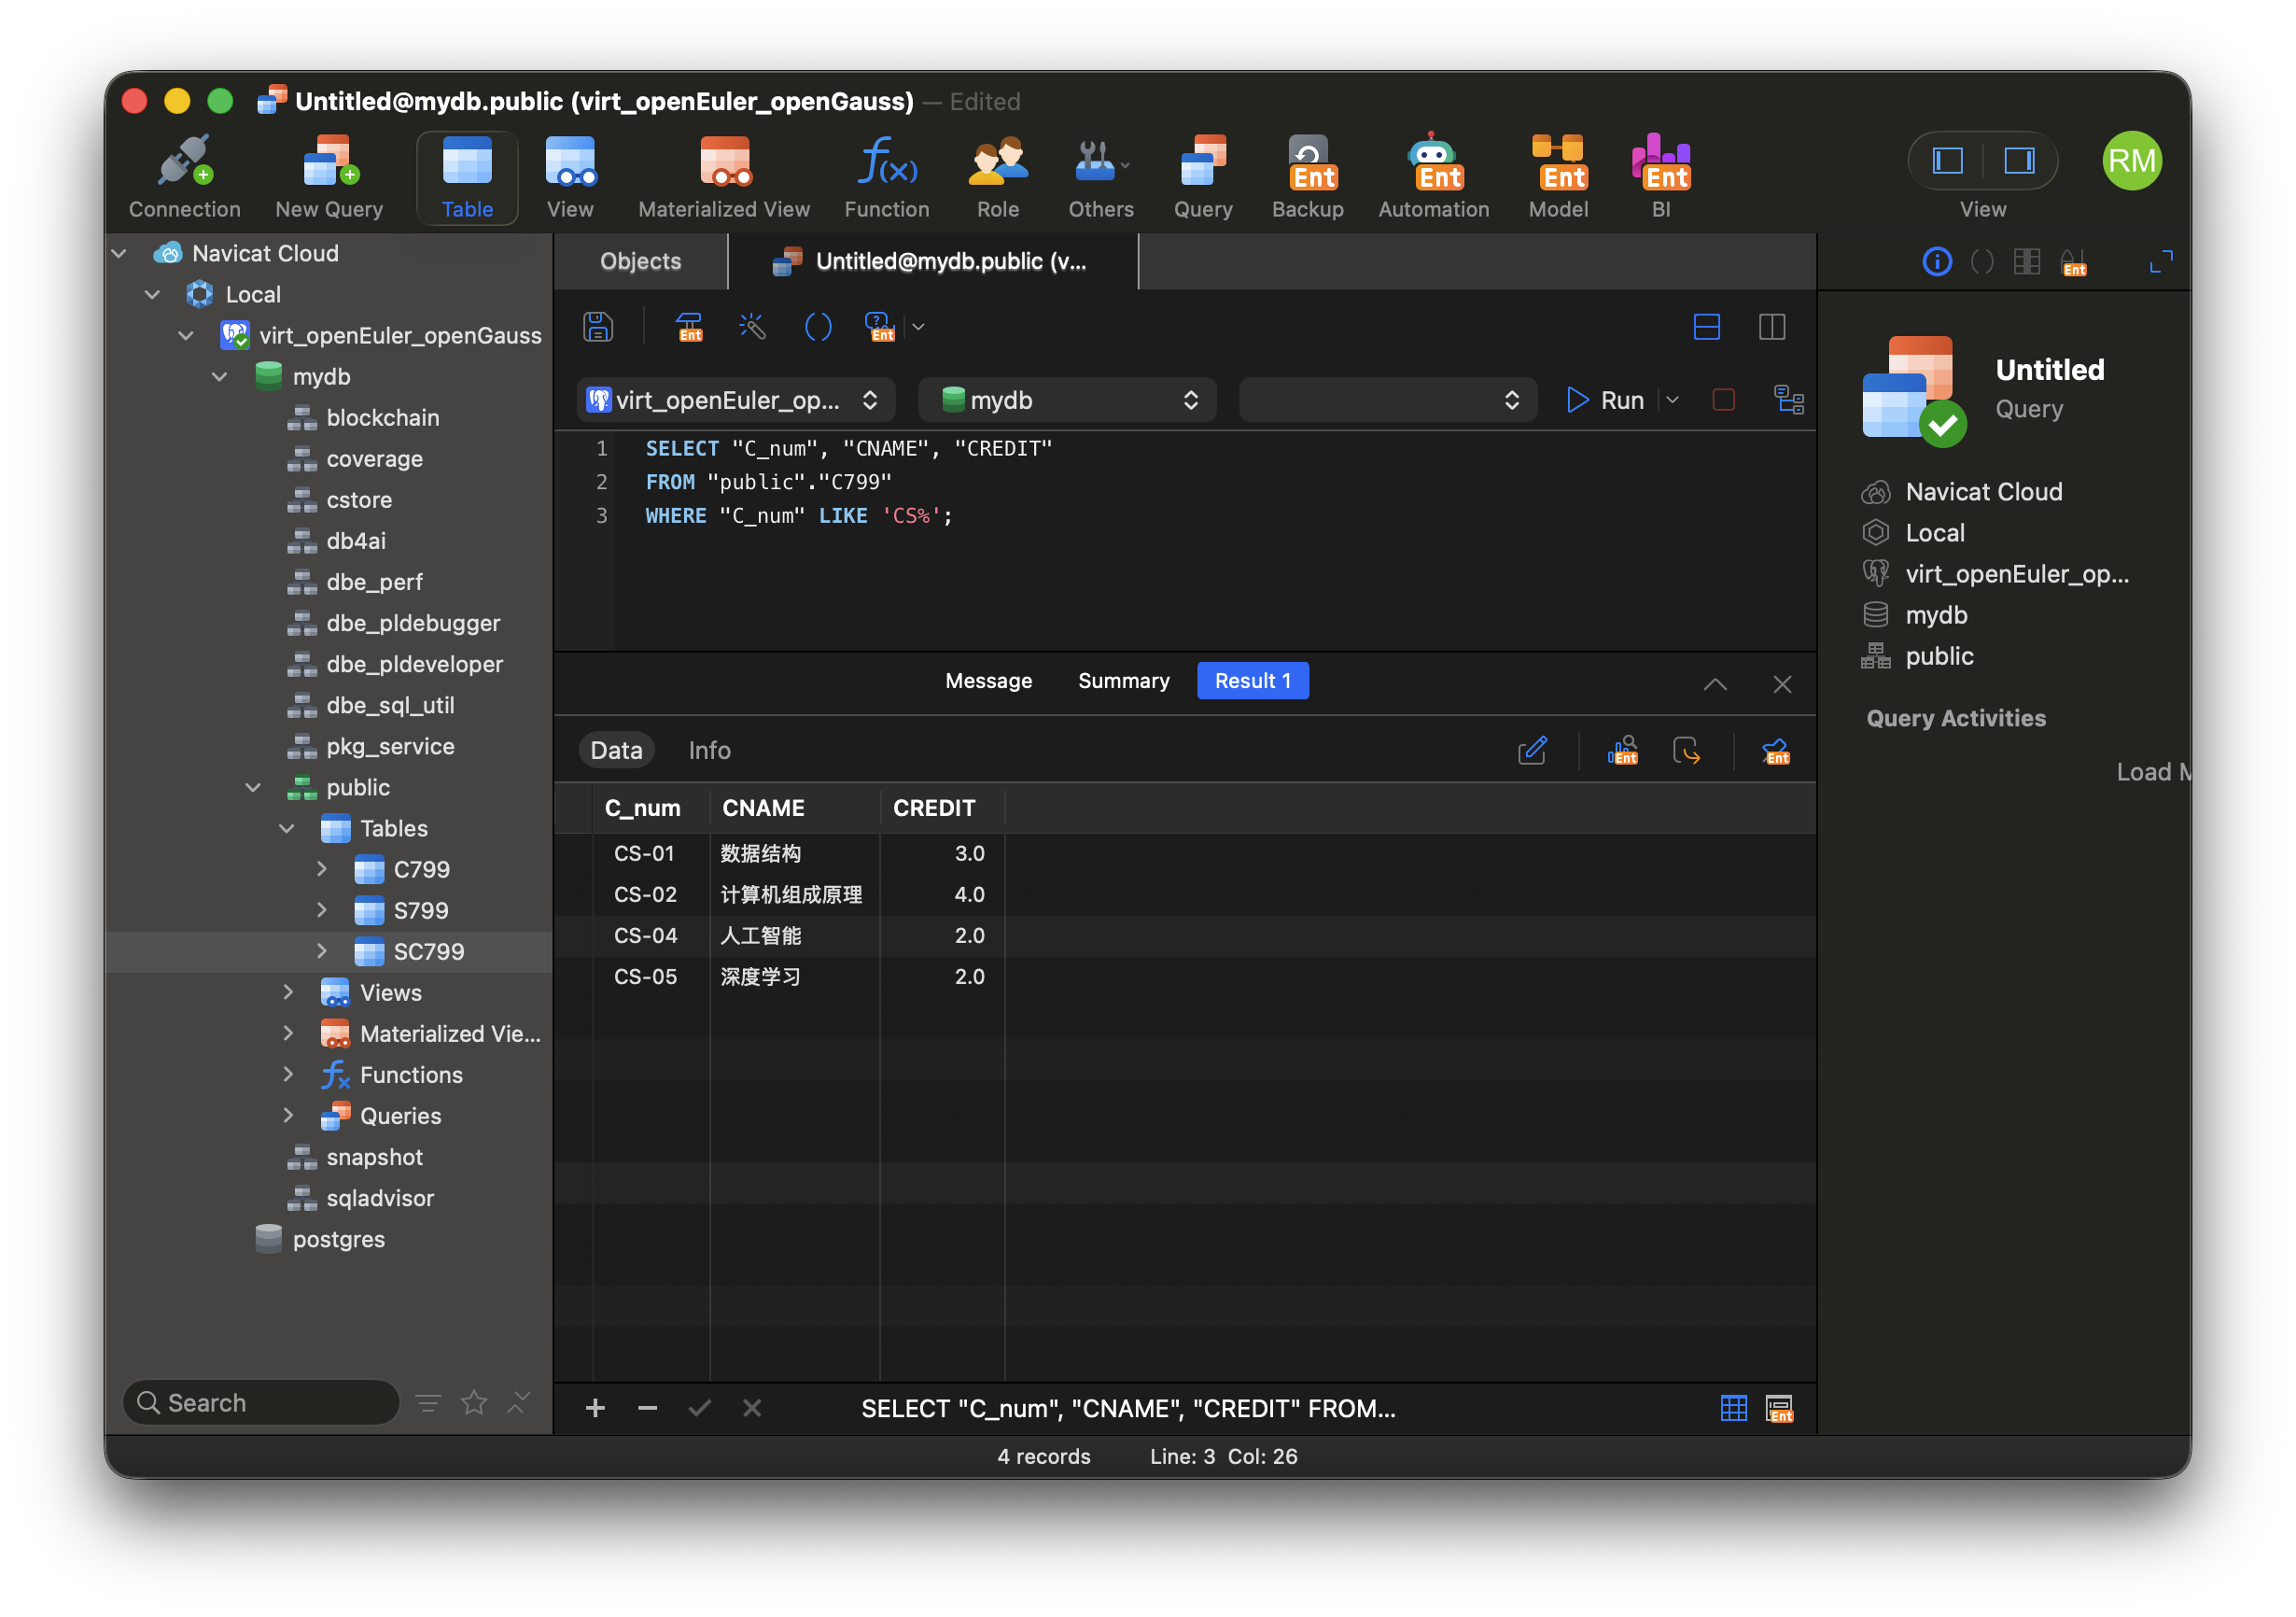
\includegraphics[width=0.88\textwidth]{images/7_3_1(1).png}
\caption{查询计算机系（CS）课程的编号、名称及学分数，共返回 4 条记录}
\label{fig:q1}
\end{figure}

查询结果返回 CS-01（数据结构，3 学分）、CS-02（计算机组成原理，4 学分）、CS-04（人工智能，2 学分）、CS-05（深度学习，2 学分）共 4 门课程，均以"CS"为课程编号前缀。

\paragraph{(2) 查询未选修课程"CS-05"的男生学号及其已选各课程编号、成绩}

\textbf{思路}：使用 \texttt{NOT IN} 子查询排除已选修 CS-05 的学号集合，在外层通过 \texttt{JOIN} 获取符合条件的男生的全部选课记录。

\begin{lstlisting}[style=sqlstyle]
SELECT s."S_num", sc."C_num", sc."GRADE"
FROM "public"."S799" s
JOIN "public"."SC799" sc ON s."S_num" = sc."S_num"
WHERE s."SEX" = '男'
  AND s."S_num" NOT IN (
      SELECT "S_num"
      FROM "public"."SC799"
      WHERE "C_num" = 'CS-05'
  );
\end{lstlisting}

\begin{figure}[H]
\centering
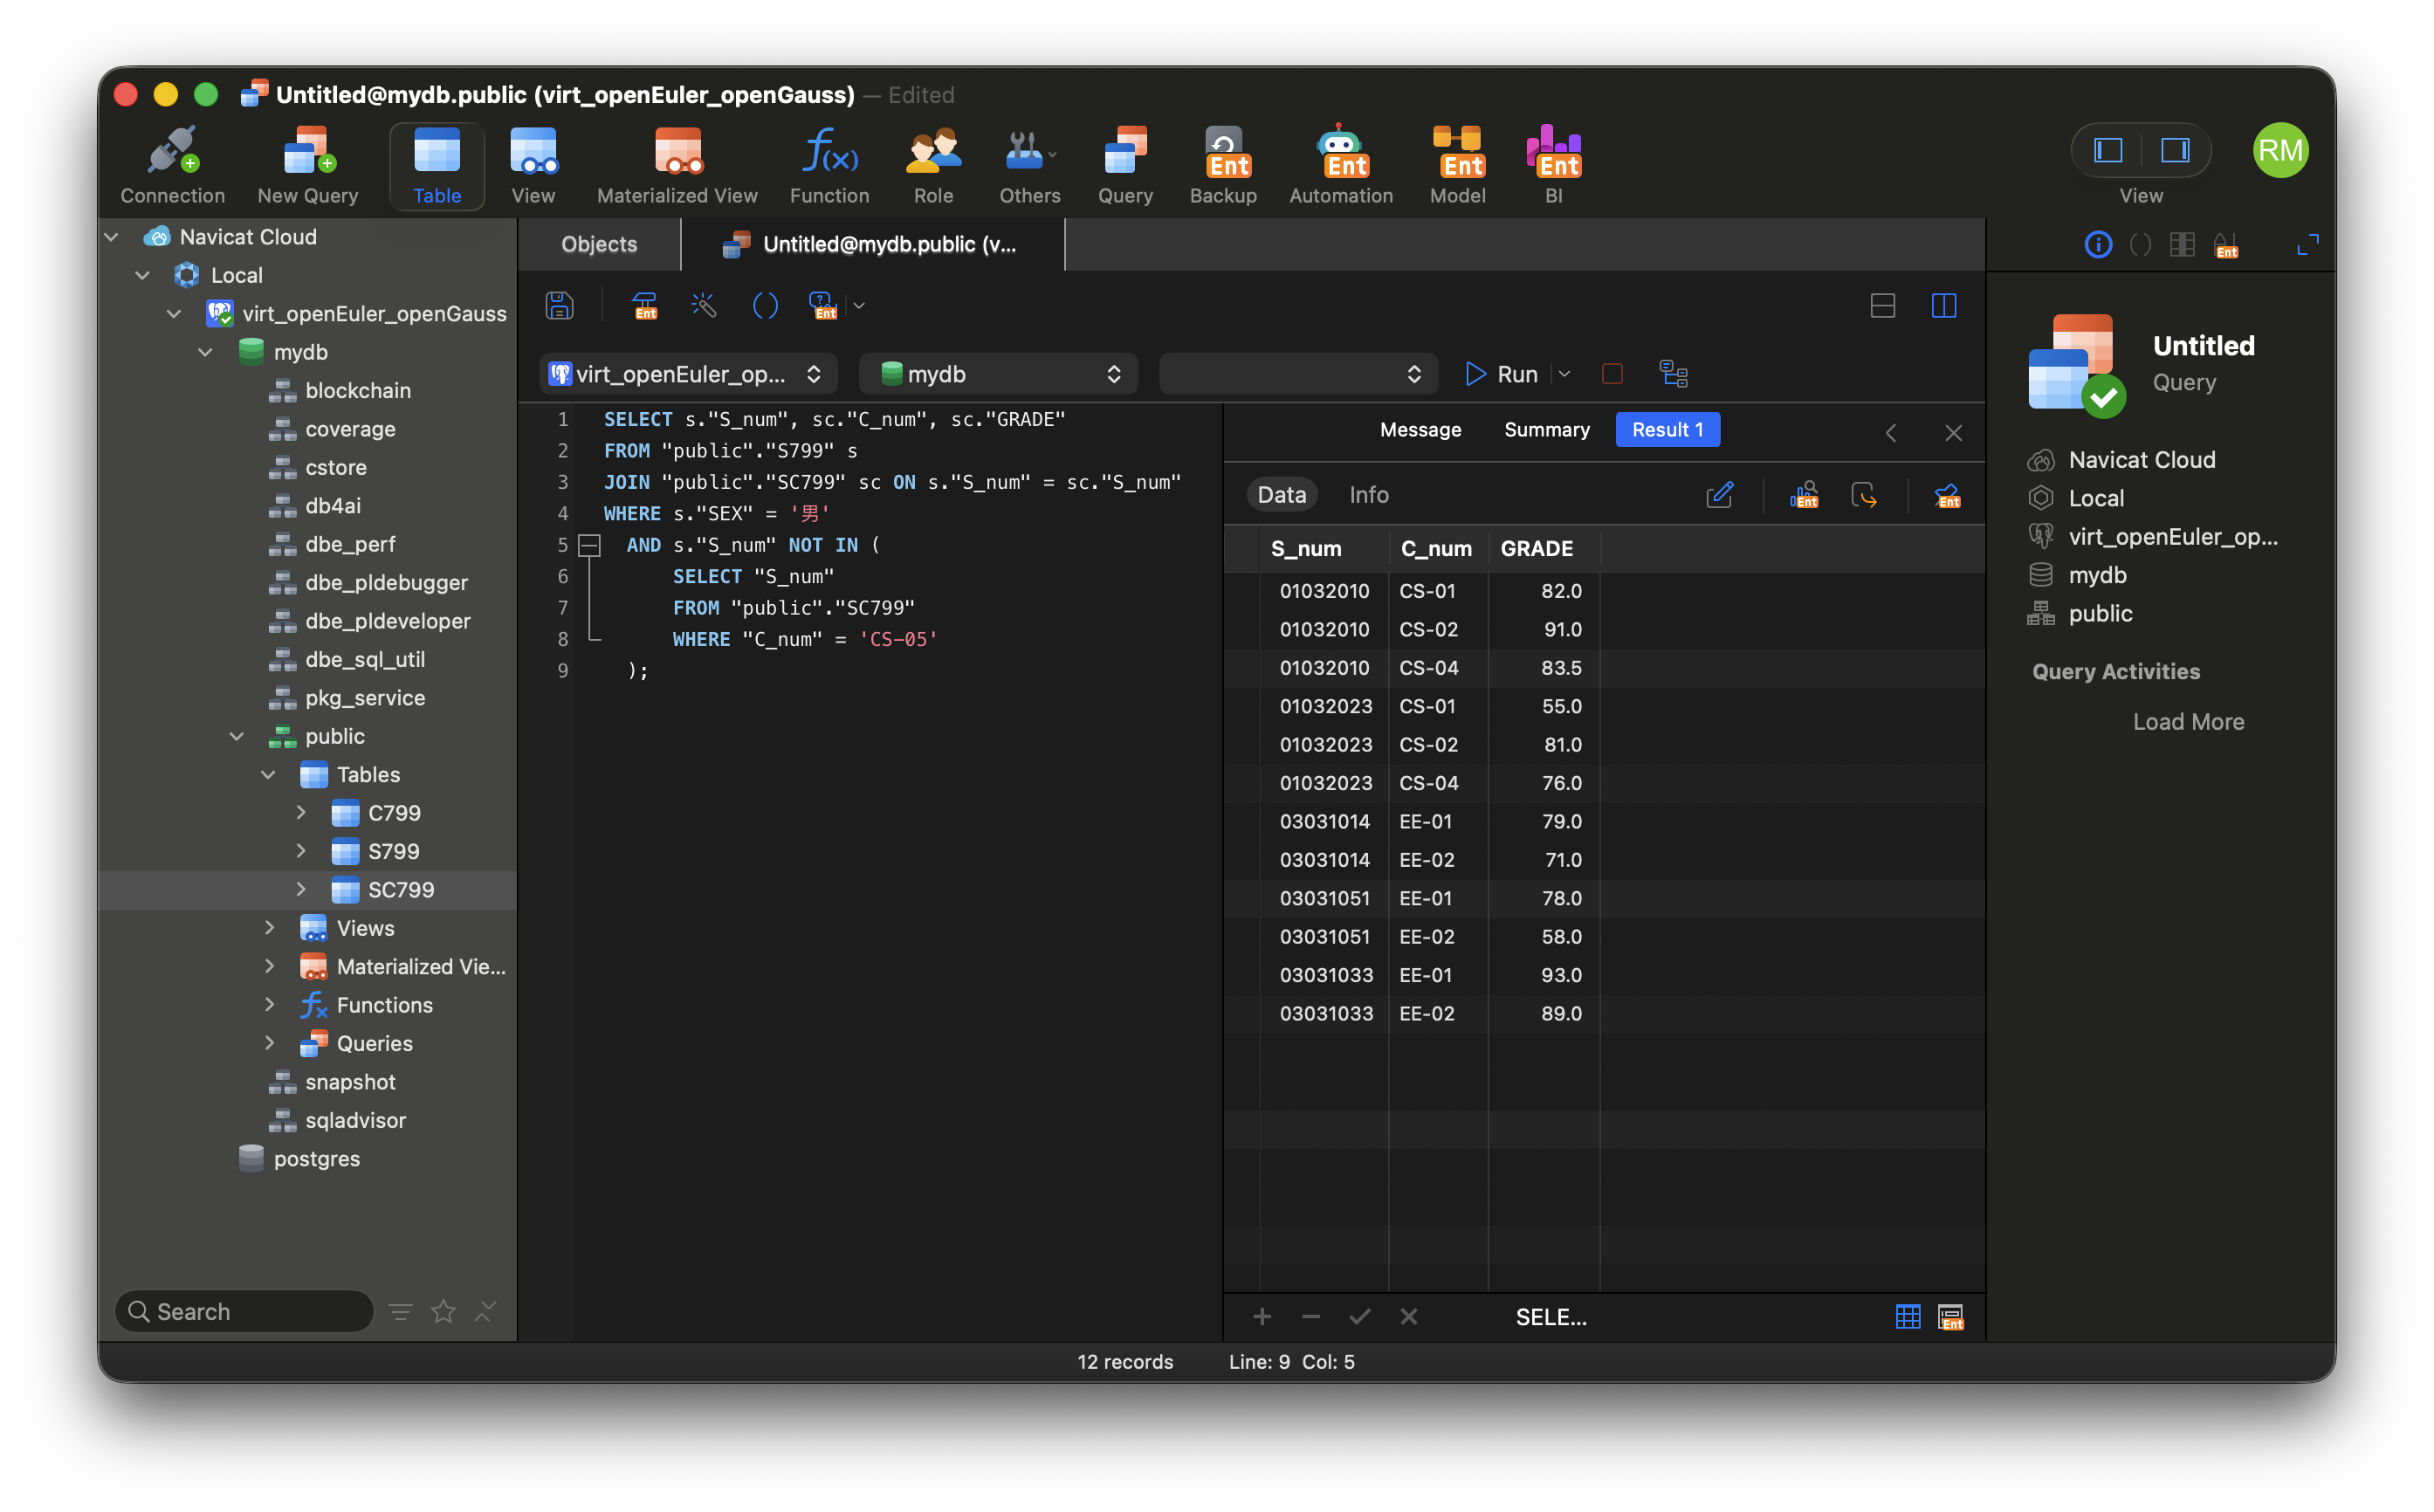
\includegraphics[width=0.88\textwidth]{images/8_3_1(2).png}
\caption{查询未选修 CS-05 的男生及其已选课程与成绩}
\label{fig:q2}
\end{figure}

子查询找出已选 CS-05 的学生（许澍，\texttt{01032112}），外层查询从结果中排除许澍，返回王涛、孙文、赵思扬、周剑、蔡明明等男生的选课记录。

\paragraph{(3) 查询 2005 年～2006 年出生学生的基本信息}

\textbf{思路}：使用 \texttt{BETWEEN ... AND ...} 对 \texttt{BDATE} 字段进行日期范围筛选，包含两端点。

\begin{lstlisting}[style=sqlstyle]
SELECT *
FROM "public"."S799"
WHERE "BDATE" BETWEEN '2005-01-01' AND '2006-12-31';
\end{lstlisting}

\begin{figure}[H]
\centering
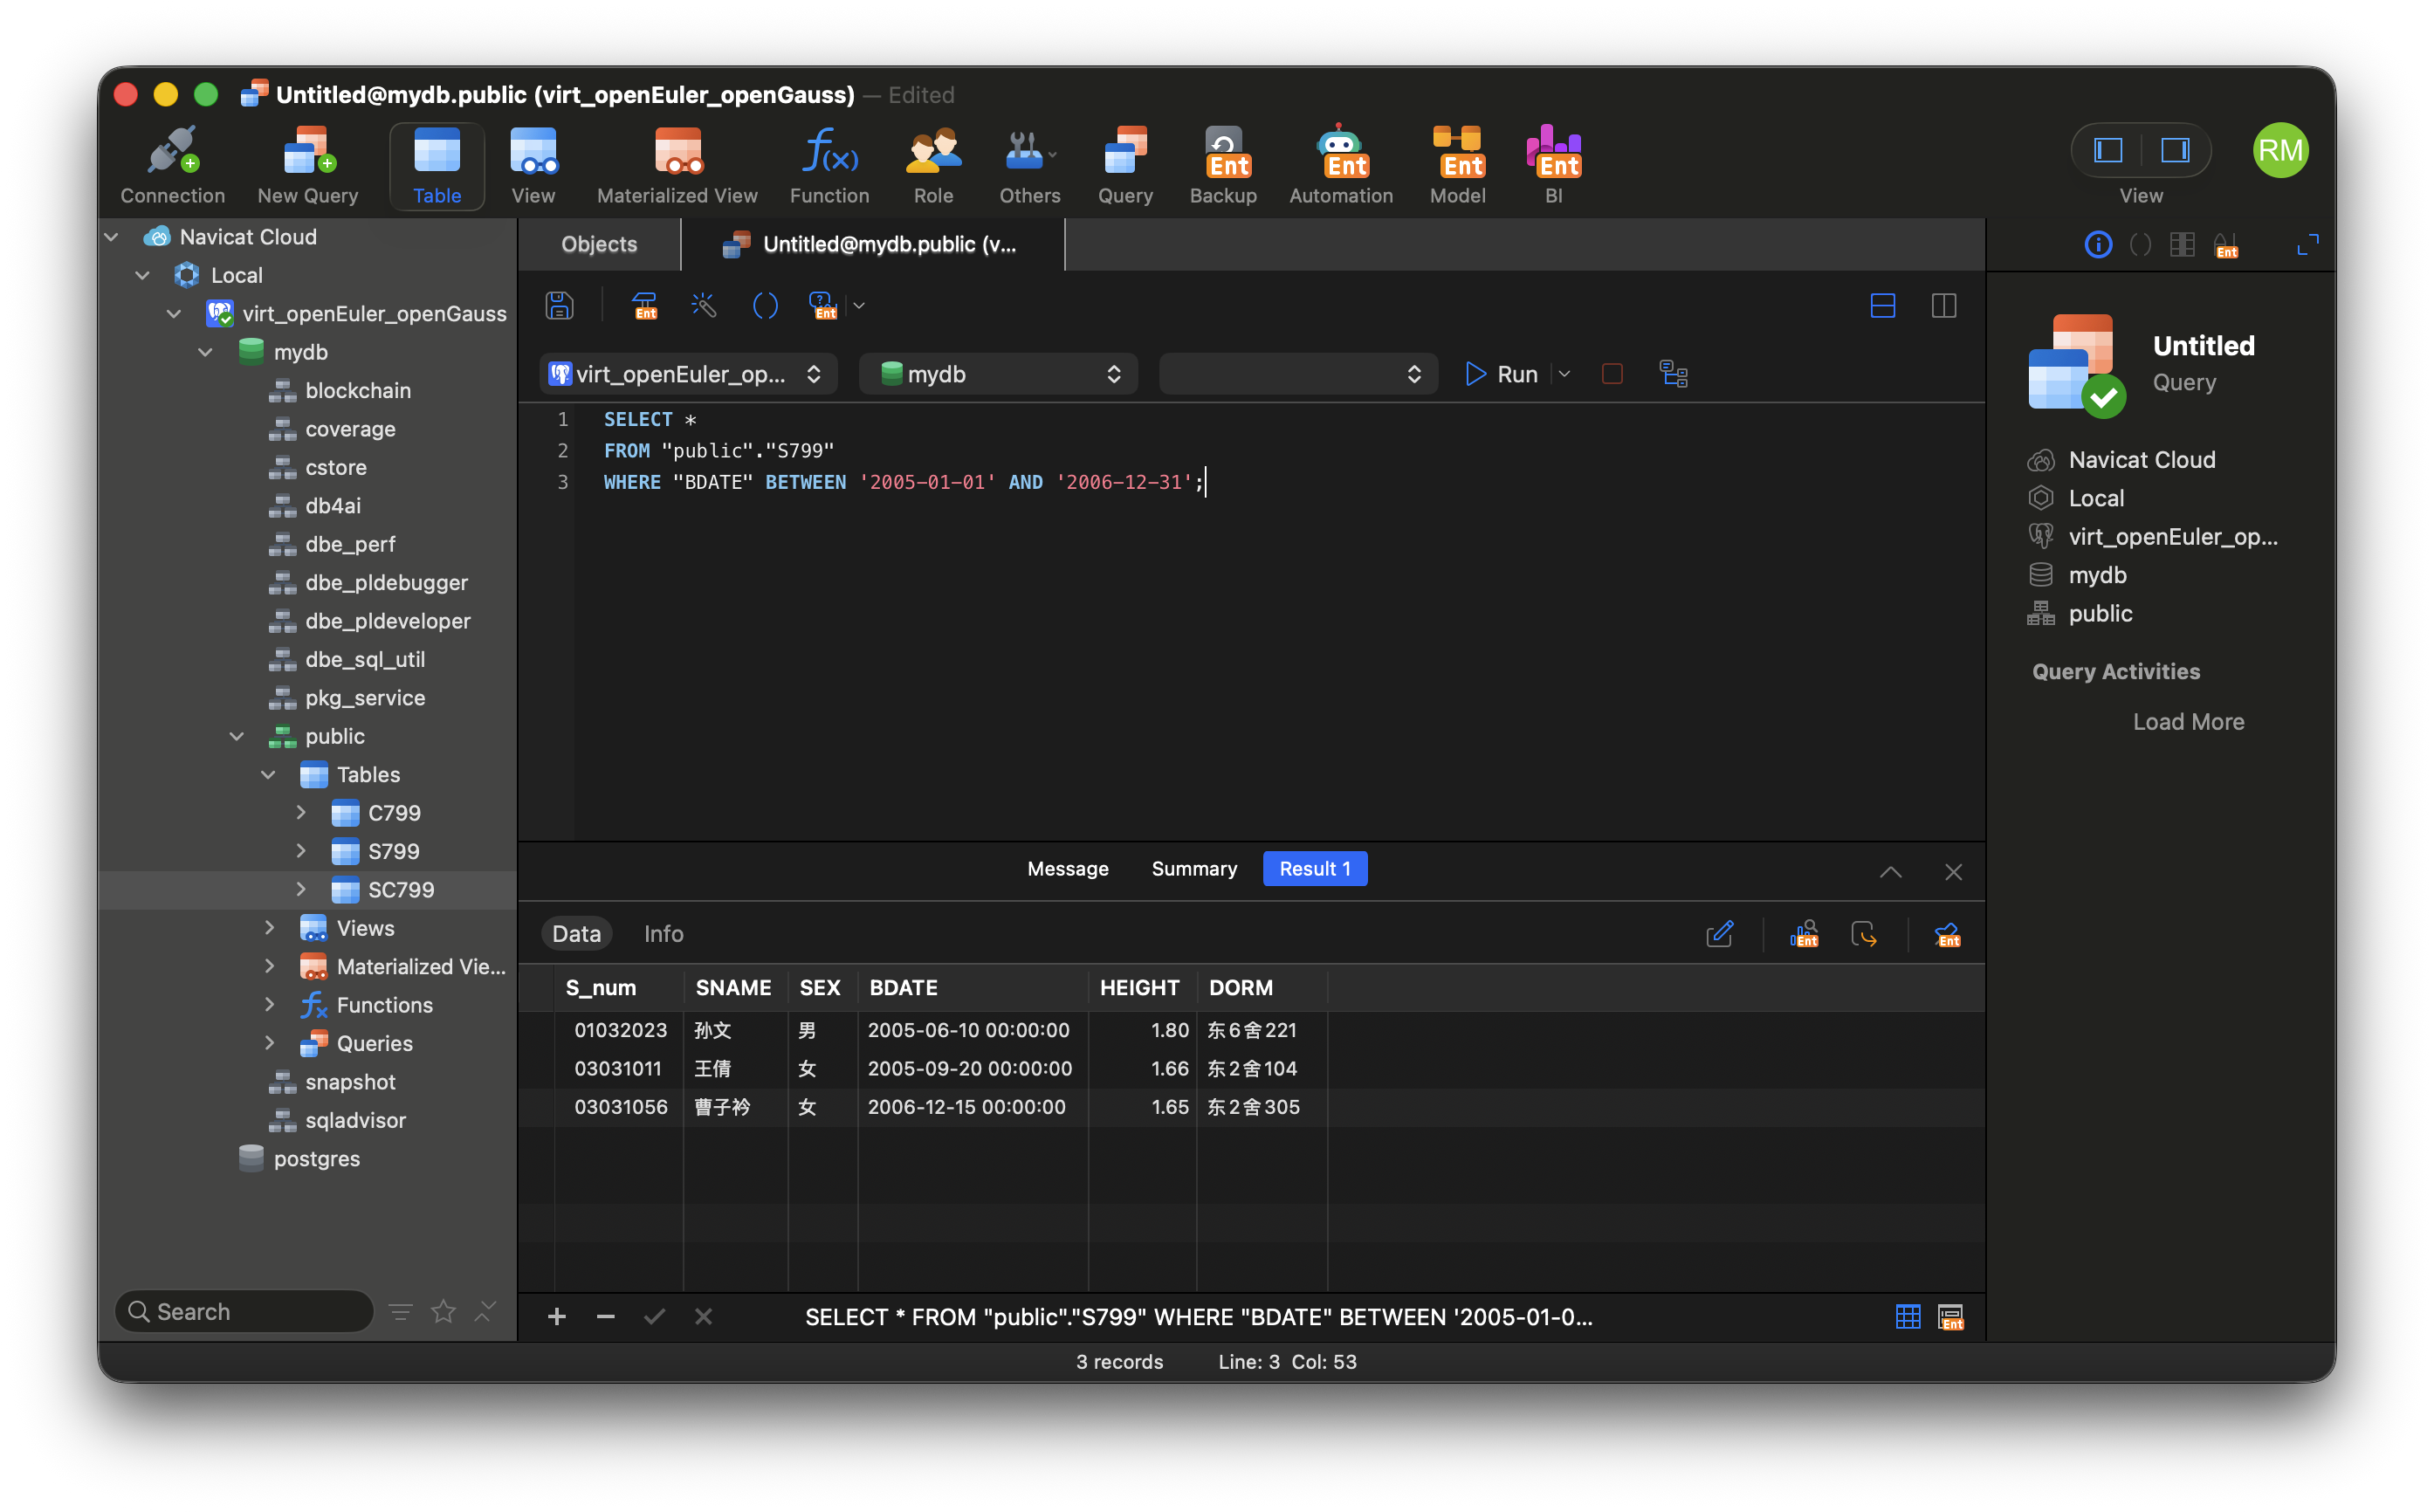
\includegraphics[width=0.88\textwidth]{images/9_3_1(3).png}
\caption{查询 2005 至 2006 年出生的学生基本信息，共 3 条记录}
\label{fig:q3}
\end{figure}

结果包含孙文（2005-06-10）、王倩（2005-09-20）、曹子衿（2006-12-15）共 3 名学生，均在目标出生年份区间内。

\paragraph{(4) 查询每位学生的学号、学生姓名及其已选修课程的学分总数}

\textbf{思路}：使用三表的 \texttt{LEFT JOIN}，确保未选任何课程的学生也出现在结果中（学分总数显示为 0）。\texttt{COALESCE} 函数将聚合结果为 \texttt{NULL} 的情形替换为 0。

\begin{lstlisting}[style=sqlstyle]
SELECT s."S_num", s."SNAME",
       COALESCE(SUM(c."CREDIT"), 0) AS "TOTAL_CREDIT"
FROM "public"."S799" s
LEFT JOIN "public"."SC799" sc ON s."S_num" = sc."S_num"
LEFT JOIN "public"."C799"  c  ON sc."C_num" = c."C_num"
GROUP BY s."S_num", s."SNAME";
\end{lstlisting}

\begin{figure}[H]
\centering
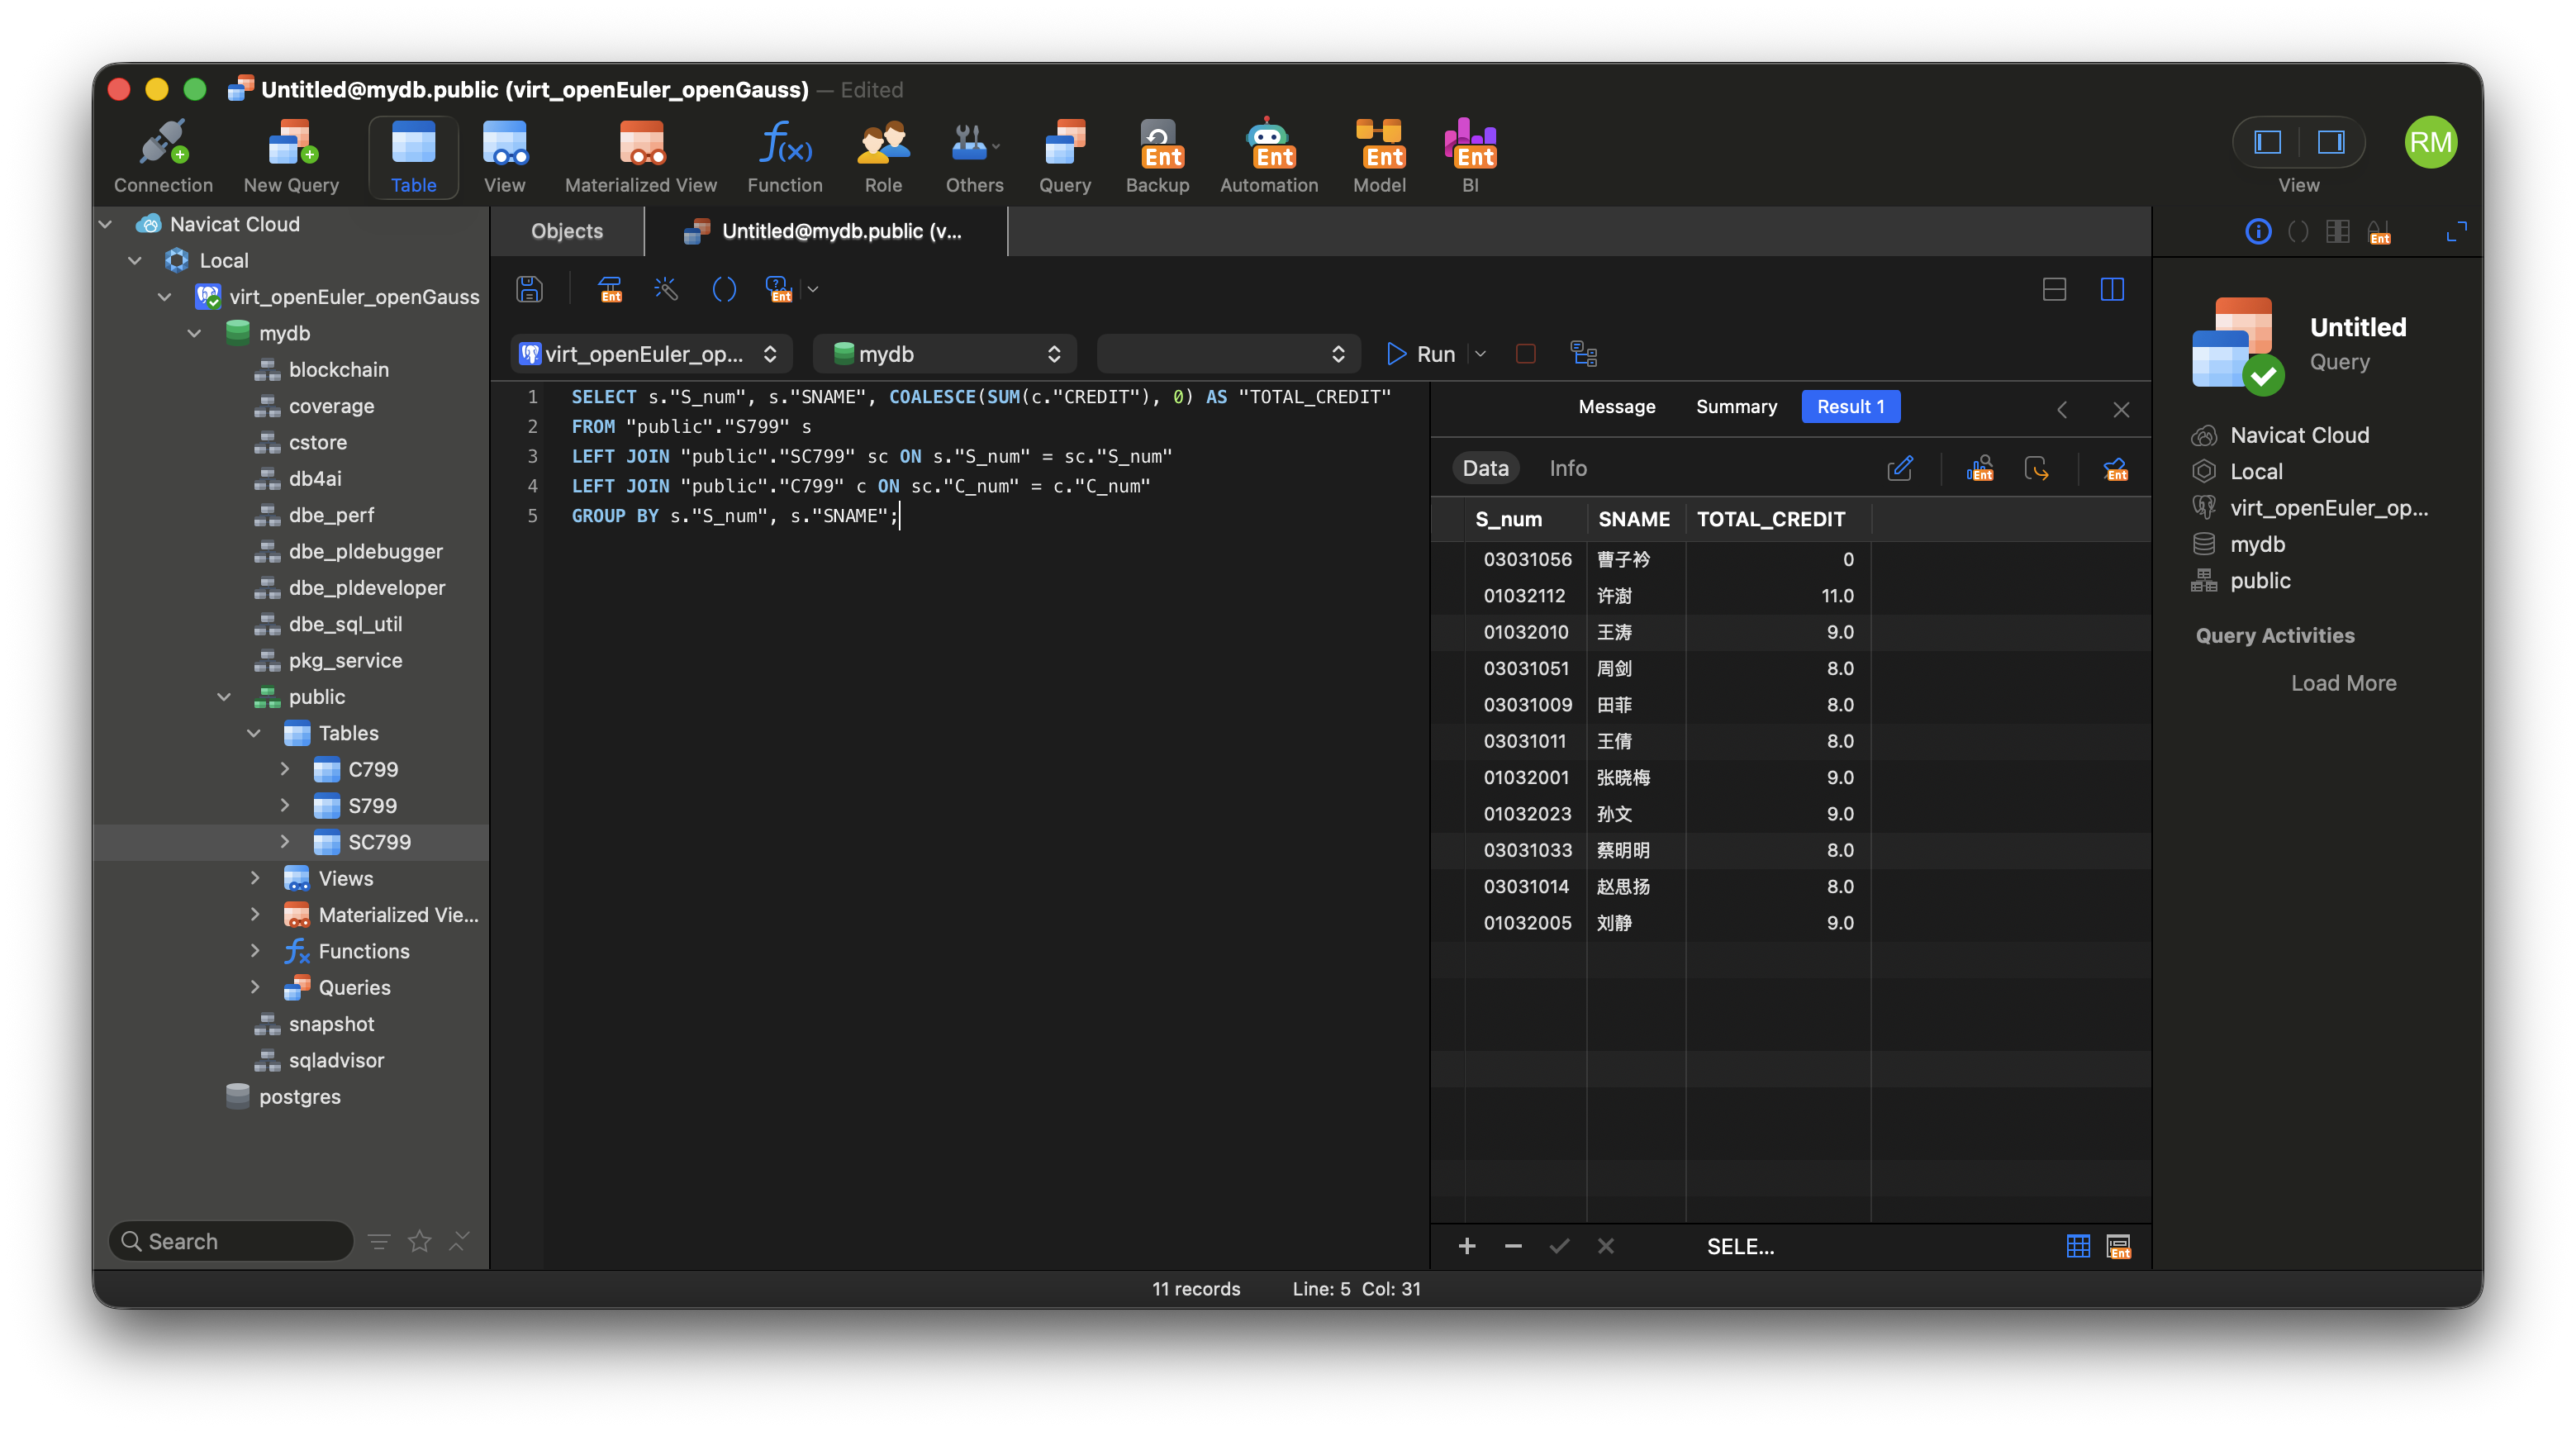
\includegraphics[width=0.88\textwidth]{images/10_3_1(4).png}
\caption{查询每位学生的学号、姓名及已选修课程总学分}
\label{fig:q4}
\end{figure}

结果展示了全部 11 名学生的总学分情况。以许澍为例，选修了 CS-01（3）、CS-02（4）、CS-04（2）、CS-05（2），总学分为 11；未选课的学生则显示总学分为 0。

\paragraph{(5) 查询选修课程"CS-01"的学生中成绩第二高的学生学号}

\textbf{思路}：先用 \texttt{WHERE} 筛选 CS-01 且成绩非空的记录，按成绩降序排列，利用 \texttt{LIMIT 1 OFFSET 1} 跳过第 1 名取第 2 名。

\begin{lstlisting}[style=sqlstyle]
SELECT "S_num"
FROM "public"."SC799"
WHERE "C_num" = 'CS-01' AND "GRADE" IS NOT NULL
ORDER BY "GRADE" DESC
LIMIT 1 OFFSET 1;
\end{lstlisting}

\begin{figure}[H]
\centering
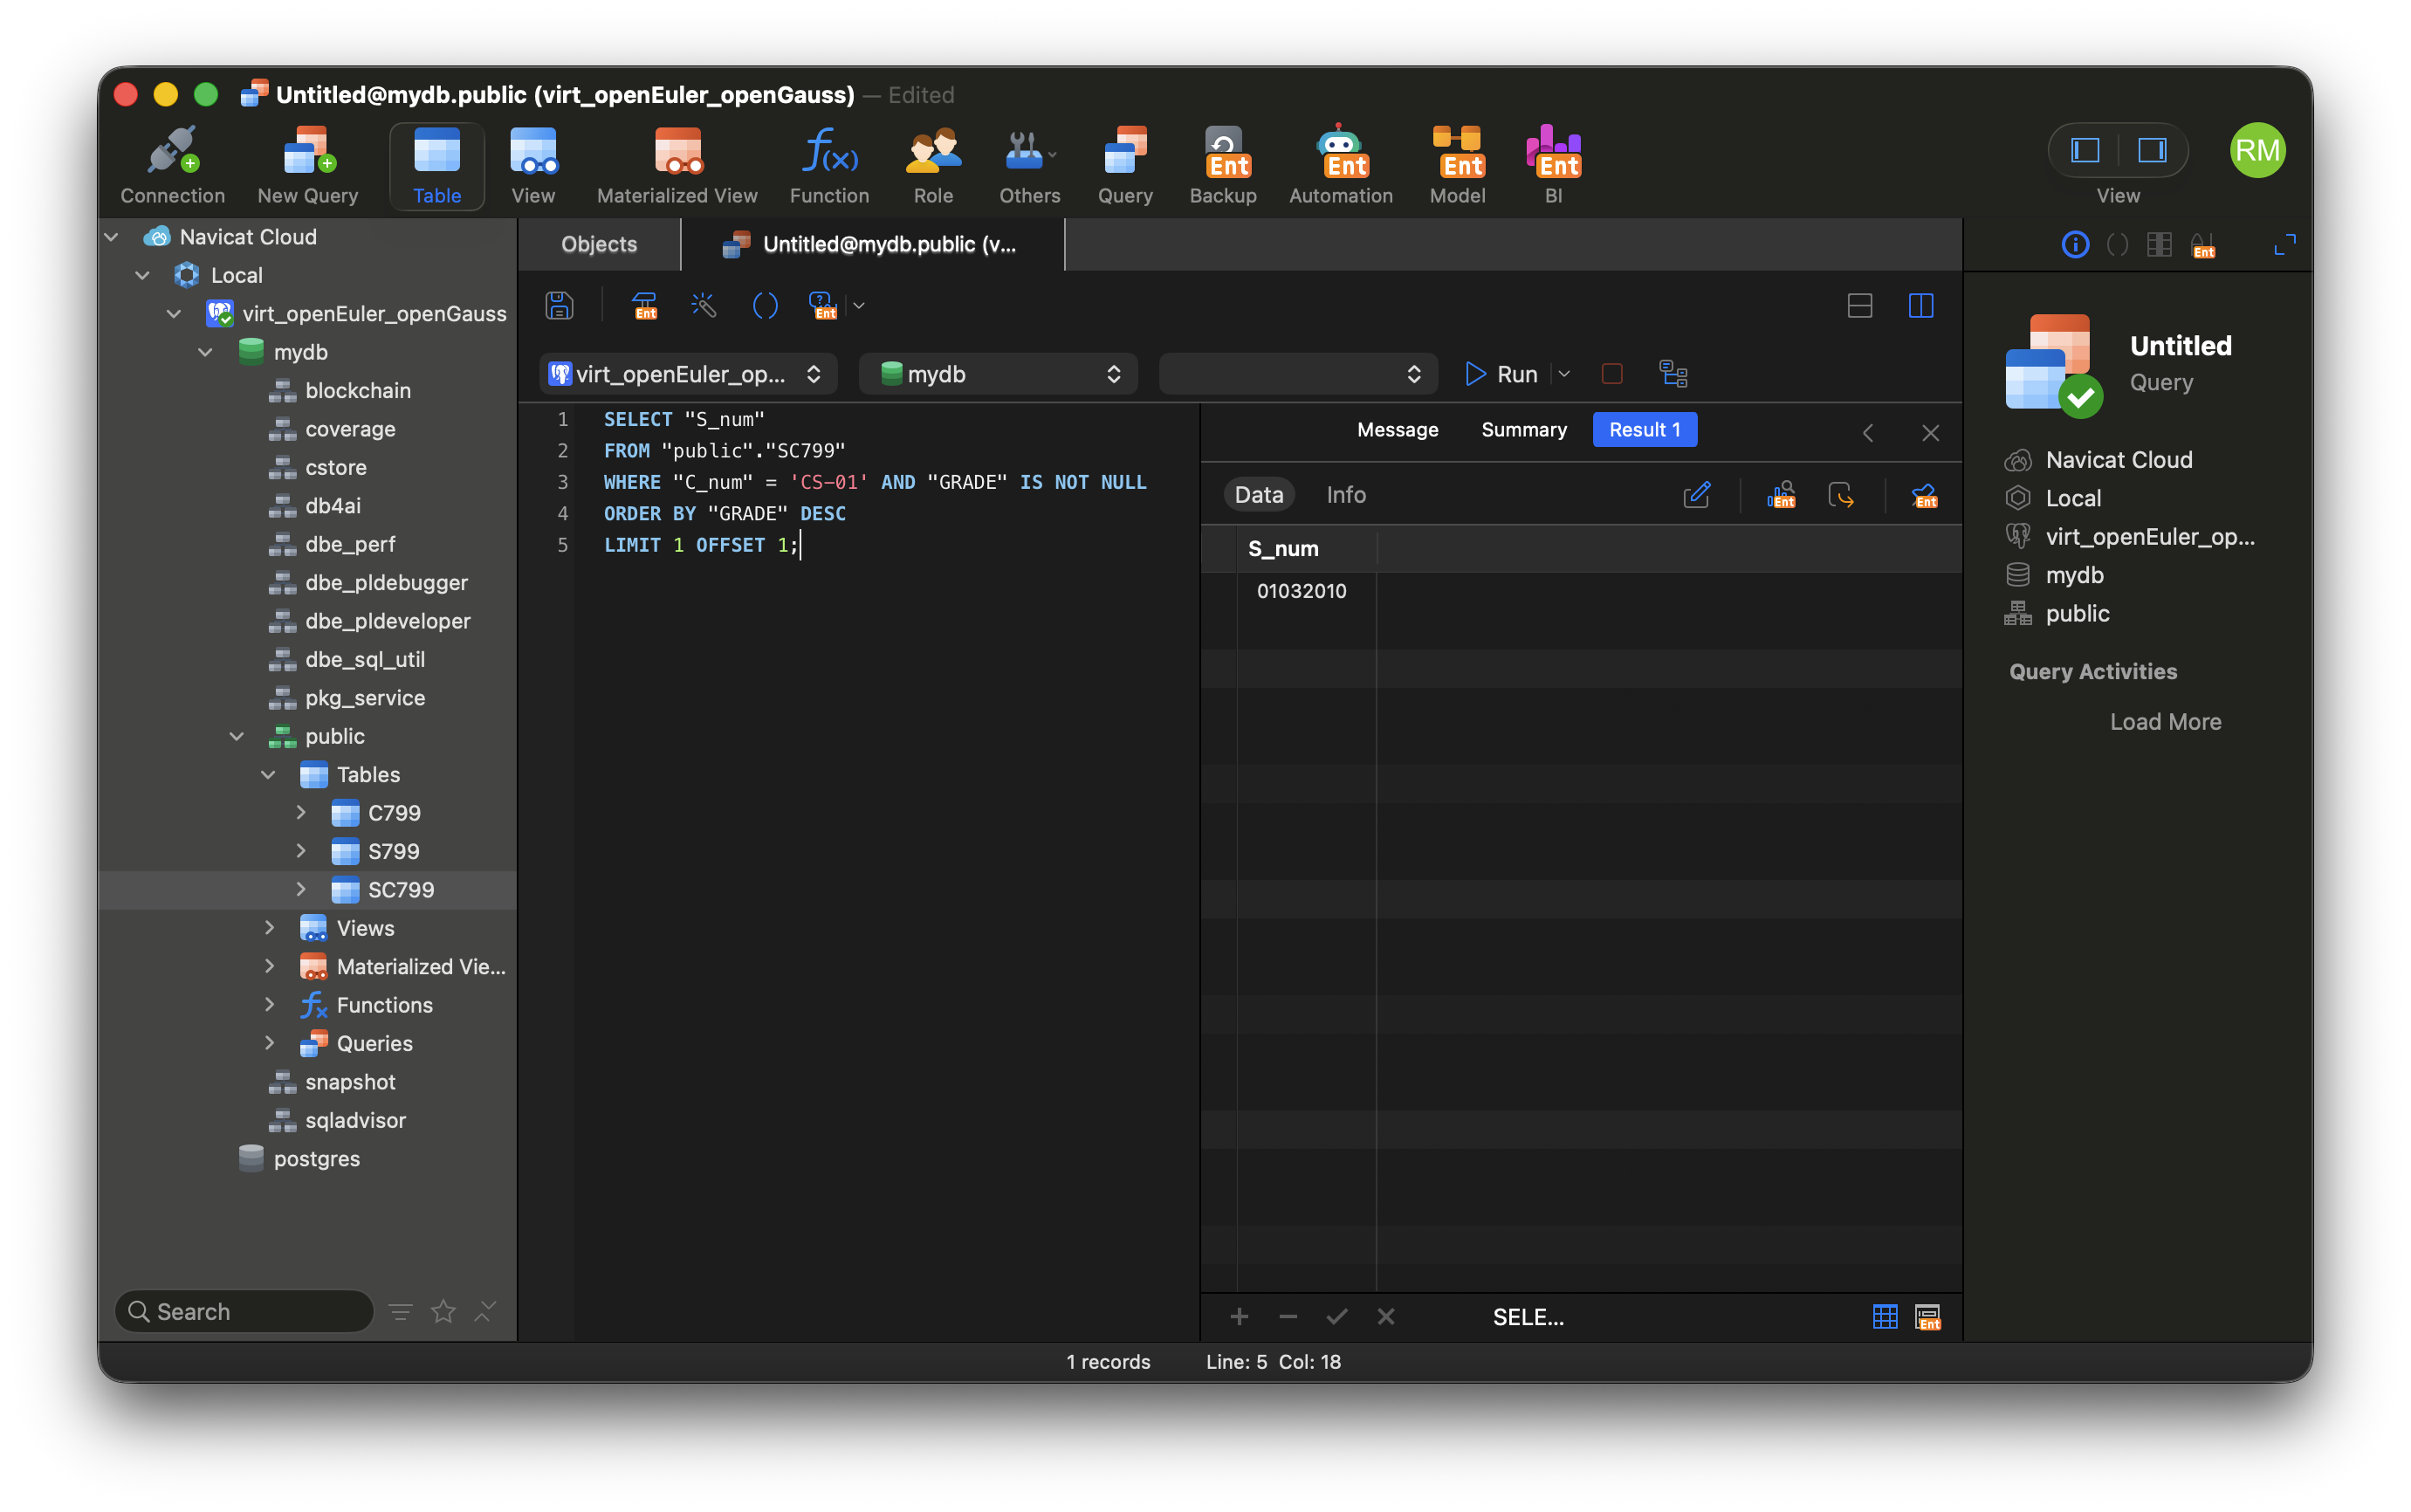
\includegraphics[width=0.88\textwidth]{images/11_3_1(5).png}
\caption{查询 CS-01 课程成绩第二高的学生学号}
\label{fig:q5}
\end{figure}

CS-01 各学生成绩降序为：许澍 88.0、王涛 82.0、张晓梅 77.5、刘静 62.0、孙文 55.0。成绩第二高为王涛（学号 \texttt{01032010}），\texttt{OFFSET 1} 精确跳过第 1 名后取到。

\paragraph{(6) 查询平均成绩低于"许澍"同学的学生学号、姓名和平均成绩，按学号降序}

\textbf{思路}：子查询计算许澍的个人平均成绩（仅统计非 NULL 记录）；外层对所有有成绩记录的学生分组求均值，用 \texttt{HAVING} 保留低于许澍均值的学生，最后按学号降序排列。

\begin{lstlisting}[style=sqlstyle]
SELECT s."S_num", s."SNAME", AVG(sc."GRADE") AS "AVG_GRADE"
FROM "public"."S799" s
JOIN "public"."SC799" sc ON s."S_num" = sc."S_num"
GROUP BY s."S_num", s."SNAME"
HAVING AVG(sc."GRADE") < (
    SELECT AVG(sc2."GRADE")
    FROM "public"."S799" s2
    JOIN "public"."SC799" sc2 ON s2."S_num" = sc2."S_num"
    WHERE s2."SNAME" = '许澍'
)
ORDER BY s."S_num" DESC;
\end{lstlisting}

\begin{figure}[H]
\centering
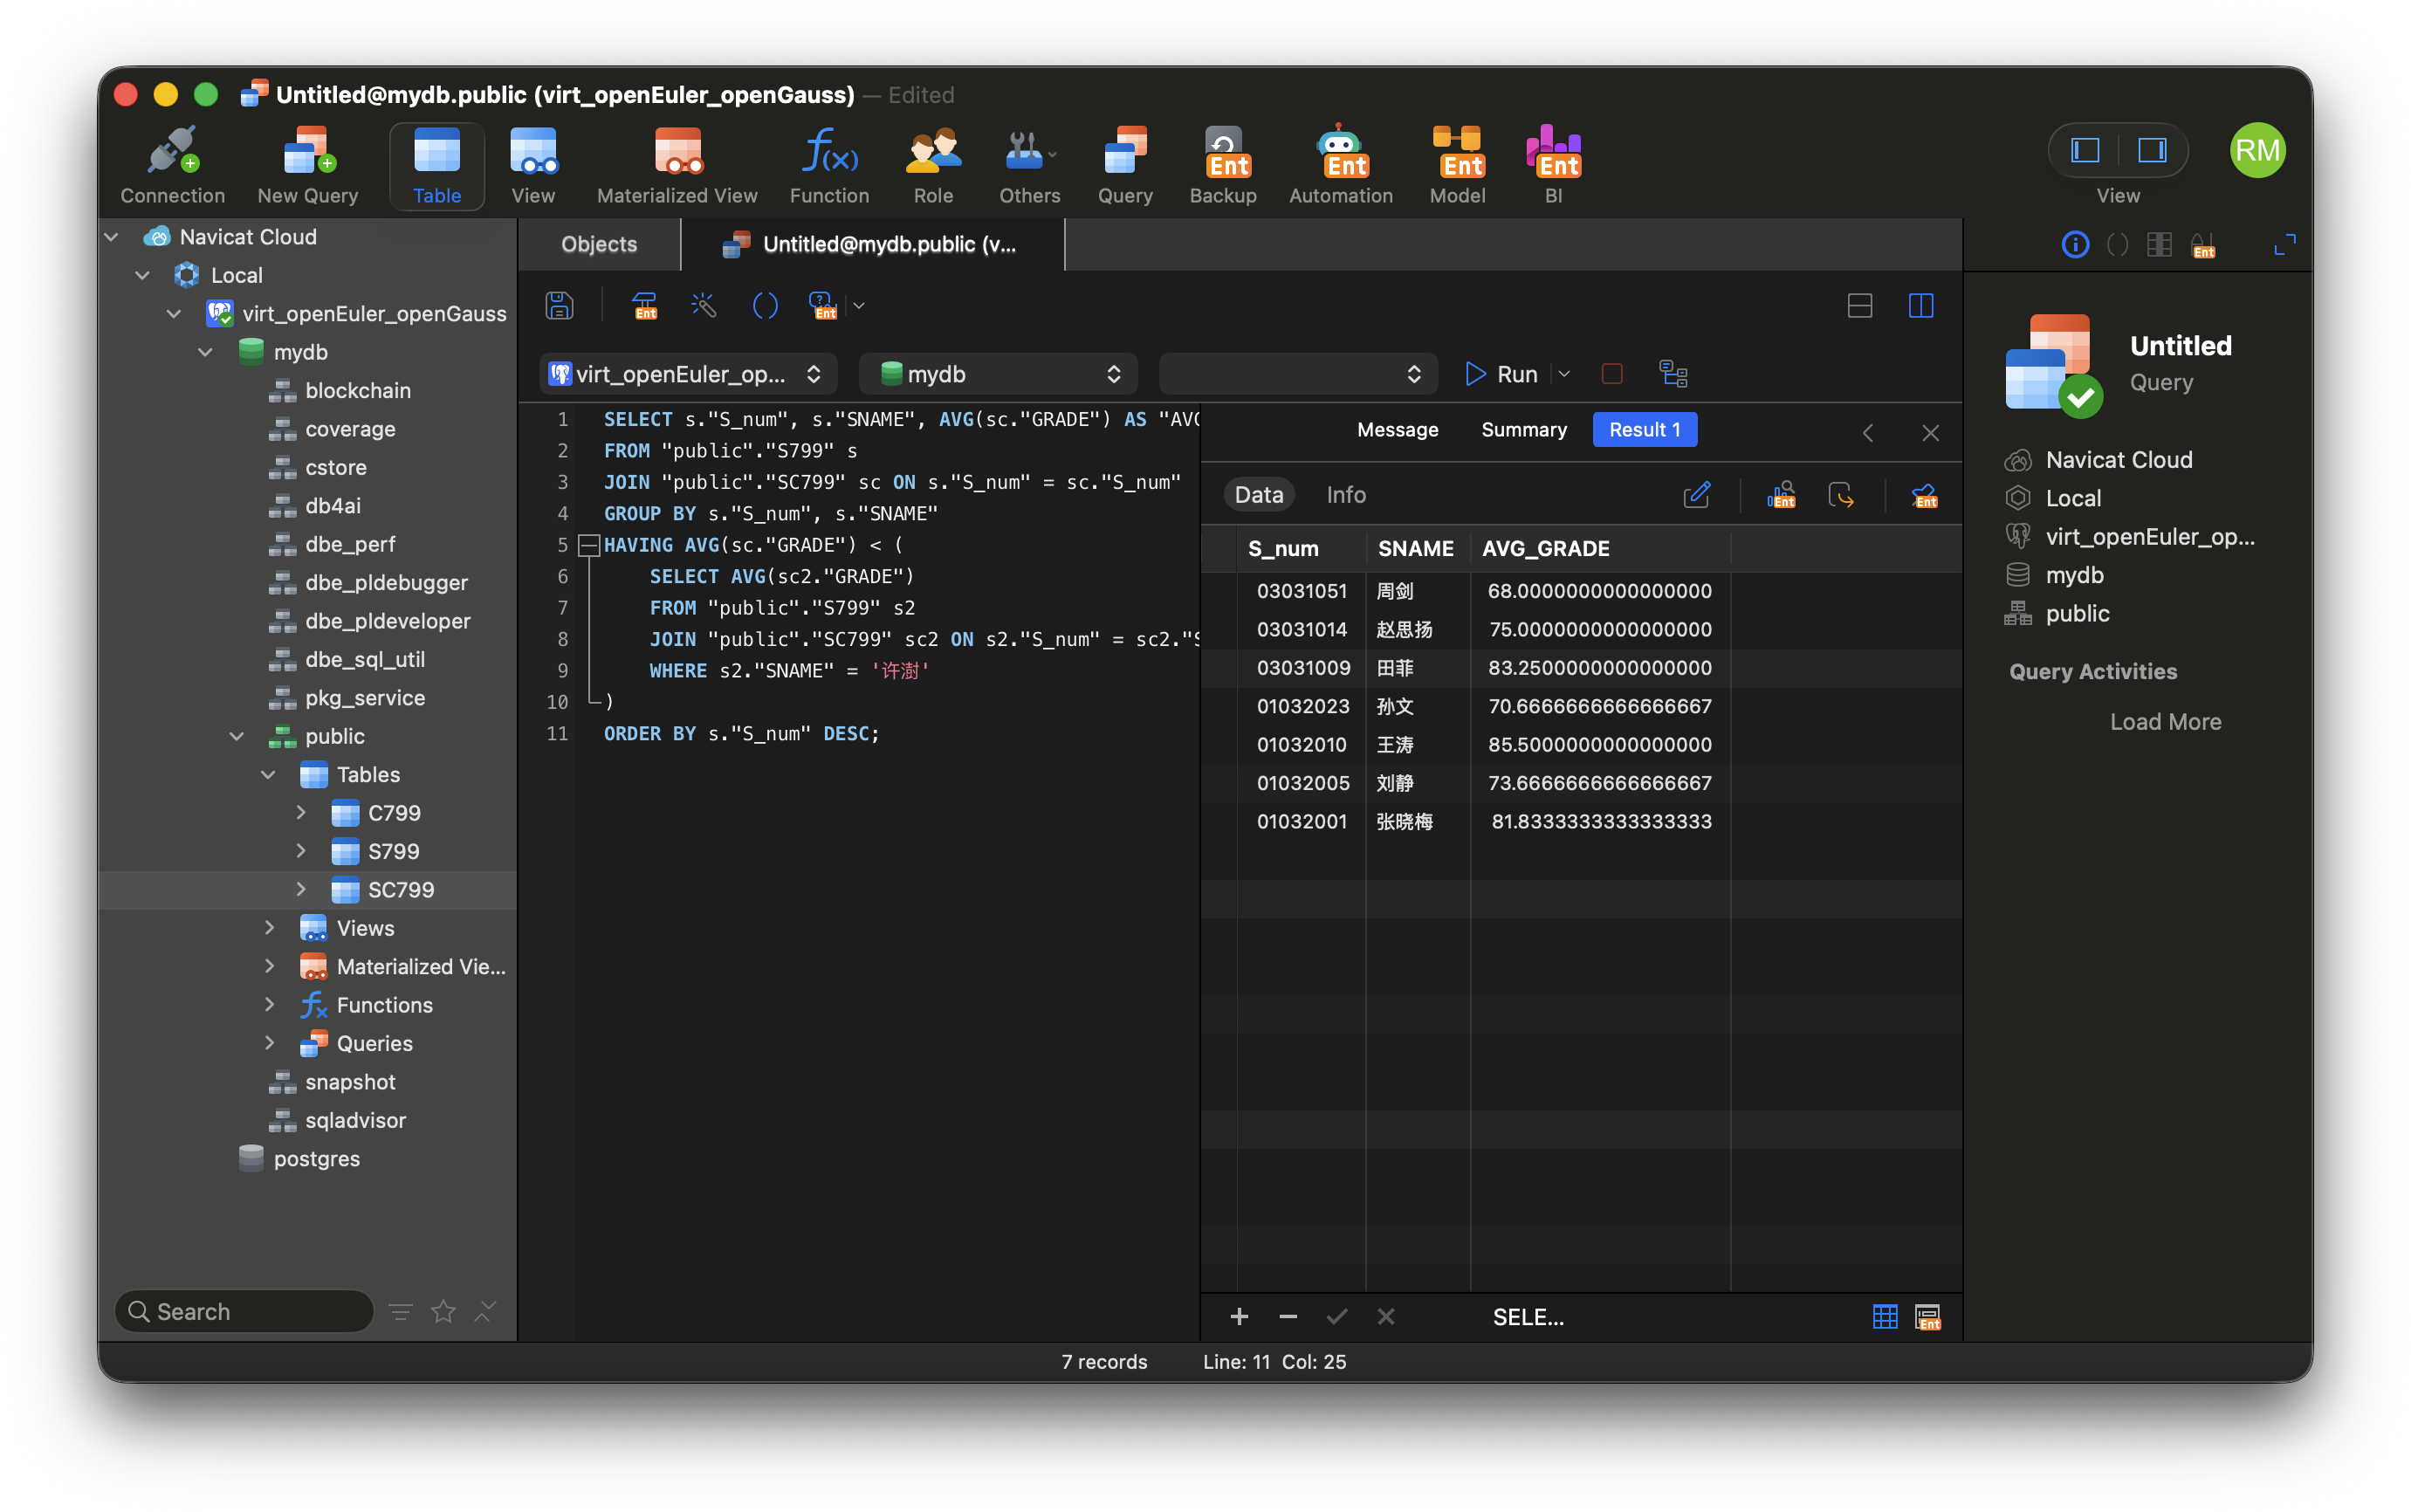
\includegraphics[width=0.88\textwidth]{images/12_3_1(6).png}
\caption{查询平均成绩低于许澍的学生（按学号降序），子查询嵌套过滤}
\label{fig:q6}
\end{figure}

许澍非 NULL 成绩：CS-01（88.0）、CS-02（91.5）、CS-04（86.0），均值约为 88.50 分。结果返回所有平均分低于此值的学生，按学号从大到小排列。

\paragraph{(7) 查询选修了计算机专业全部课程的学生姓名及已获得的学分总数}

\textbf{思路}：子查询统计 C799 中以"CS"开头的课程总数（共 4 门）；外层对每位学生统计其已选 CS 课程数量，\texttt{HAVING} 子句过滤出选满全部 4 门 CS 课程的学生，并求其所有已选课程的学分之和。

\begin{lstlisting}[style=sqlstyle]
SELECT s."SNAME", SUM(c."CREDIT") AS "TOTAL_CREDIT"
FROM "public"."S799" s
JOIN "public"."SC799" sc ON s."S_num" = sc."S_num"
JOIN "public"."C799"  c  ON sc."C_num" = c."C_num"
GROUP BY s."S_num", s."SNAME"
HAVING COUNT(CASE WHEN sc."C_num" LIKE 'CS%' THEN 1 END) = (
    SELECT COUNT(*)
    FROM "public"."C799"
    WHERE "C_num" LIKE 'CS%'
);
\end{lstlisting}

\begin{figure}[H]
\centering
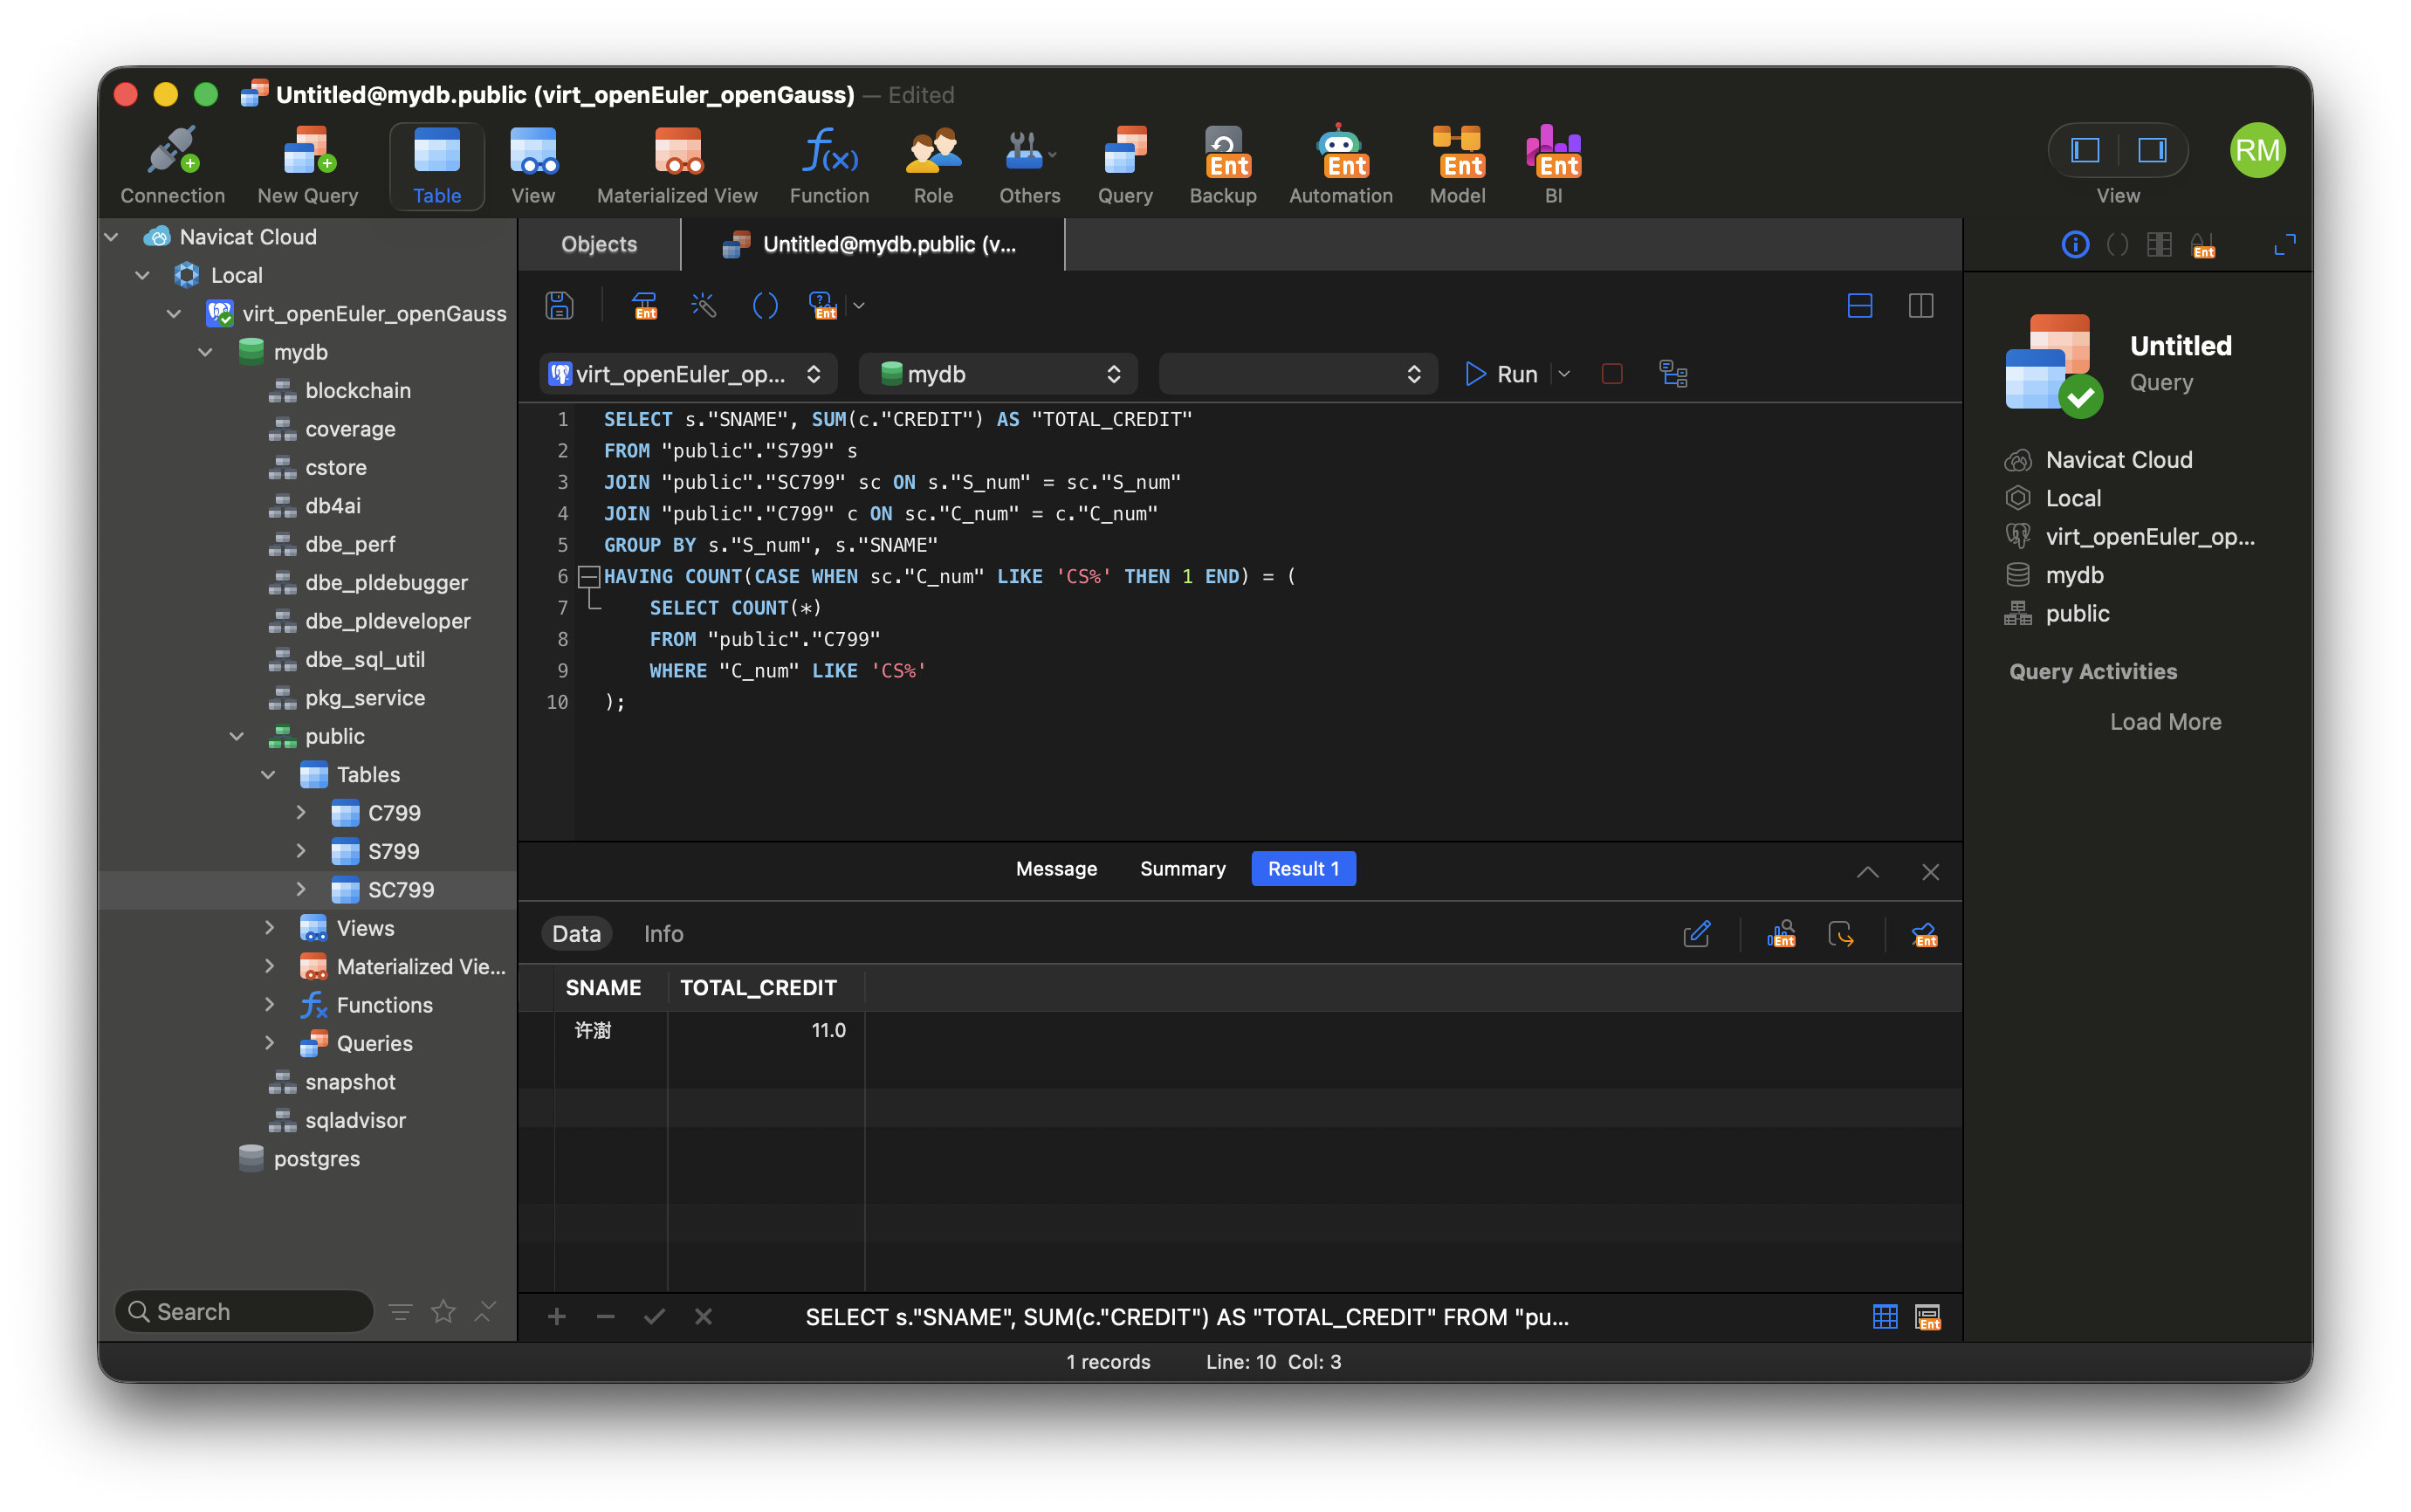
\includegraphics[width=0.88\textwidth]{images/13_3_1(7).png}
\caption{查询选修了全部计算机专业课程的学生姓名及学分总数}
\label{fig:q7}
\end{figure}

查询结果唯一：许澍，选修了全部 4 门 CS 课程（CS-01、CS-02、CS-04、CS-05），总学分为 $3+4+2+2=11$。使用 \texttt{CASE WHEN ... LIKE 'CS\%' THEN 1 END} 可以在聚合中精确计数特定前缀的课程，避免其他系别课程干扰。

\paragraph{(8) 查询选修了 3 门以上课程（含 3 门）的学生中平均成绩最高的学号及姓名}

\textbf{思路}：先用 \texttt{HAVING COUNT(sc."C\_num") >= 3} 筛选选课数不低于 3 门的学生，按平均分降序排列后用 \texttt{LIMIT 1} 取最高分学生。

\begin{lstlisting}[style=sqlstyle]
SELECT s."S_num", s."SNAME"
FROM "public"."S799" s
JOIN "public"."SC799" sc ON s."S_num" = sc."S_num"
GROUP BY s."S_num", s."SNAME"
HAVING COUNT(sc."C_num") >= 3
ORDER BY AVG(sc."GRADE") DESC
LIMIT 1;
\end{lstlisting}

\begin{figure}[H]
\centering
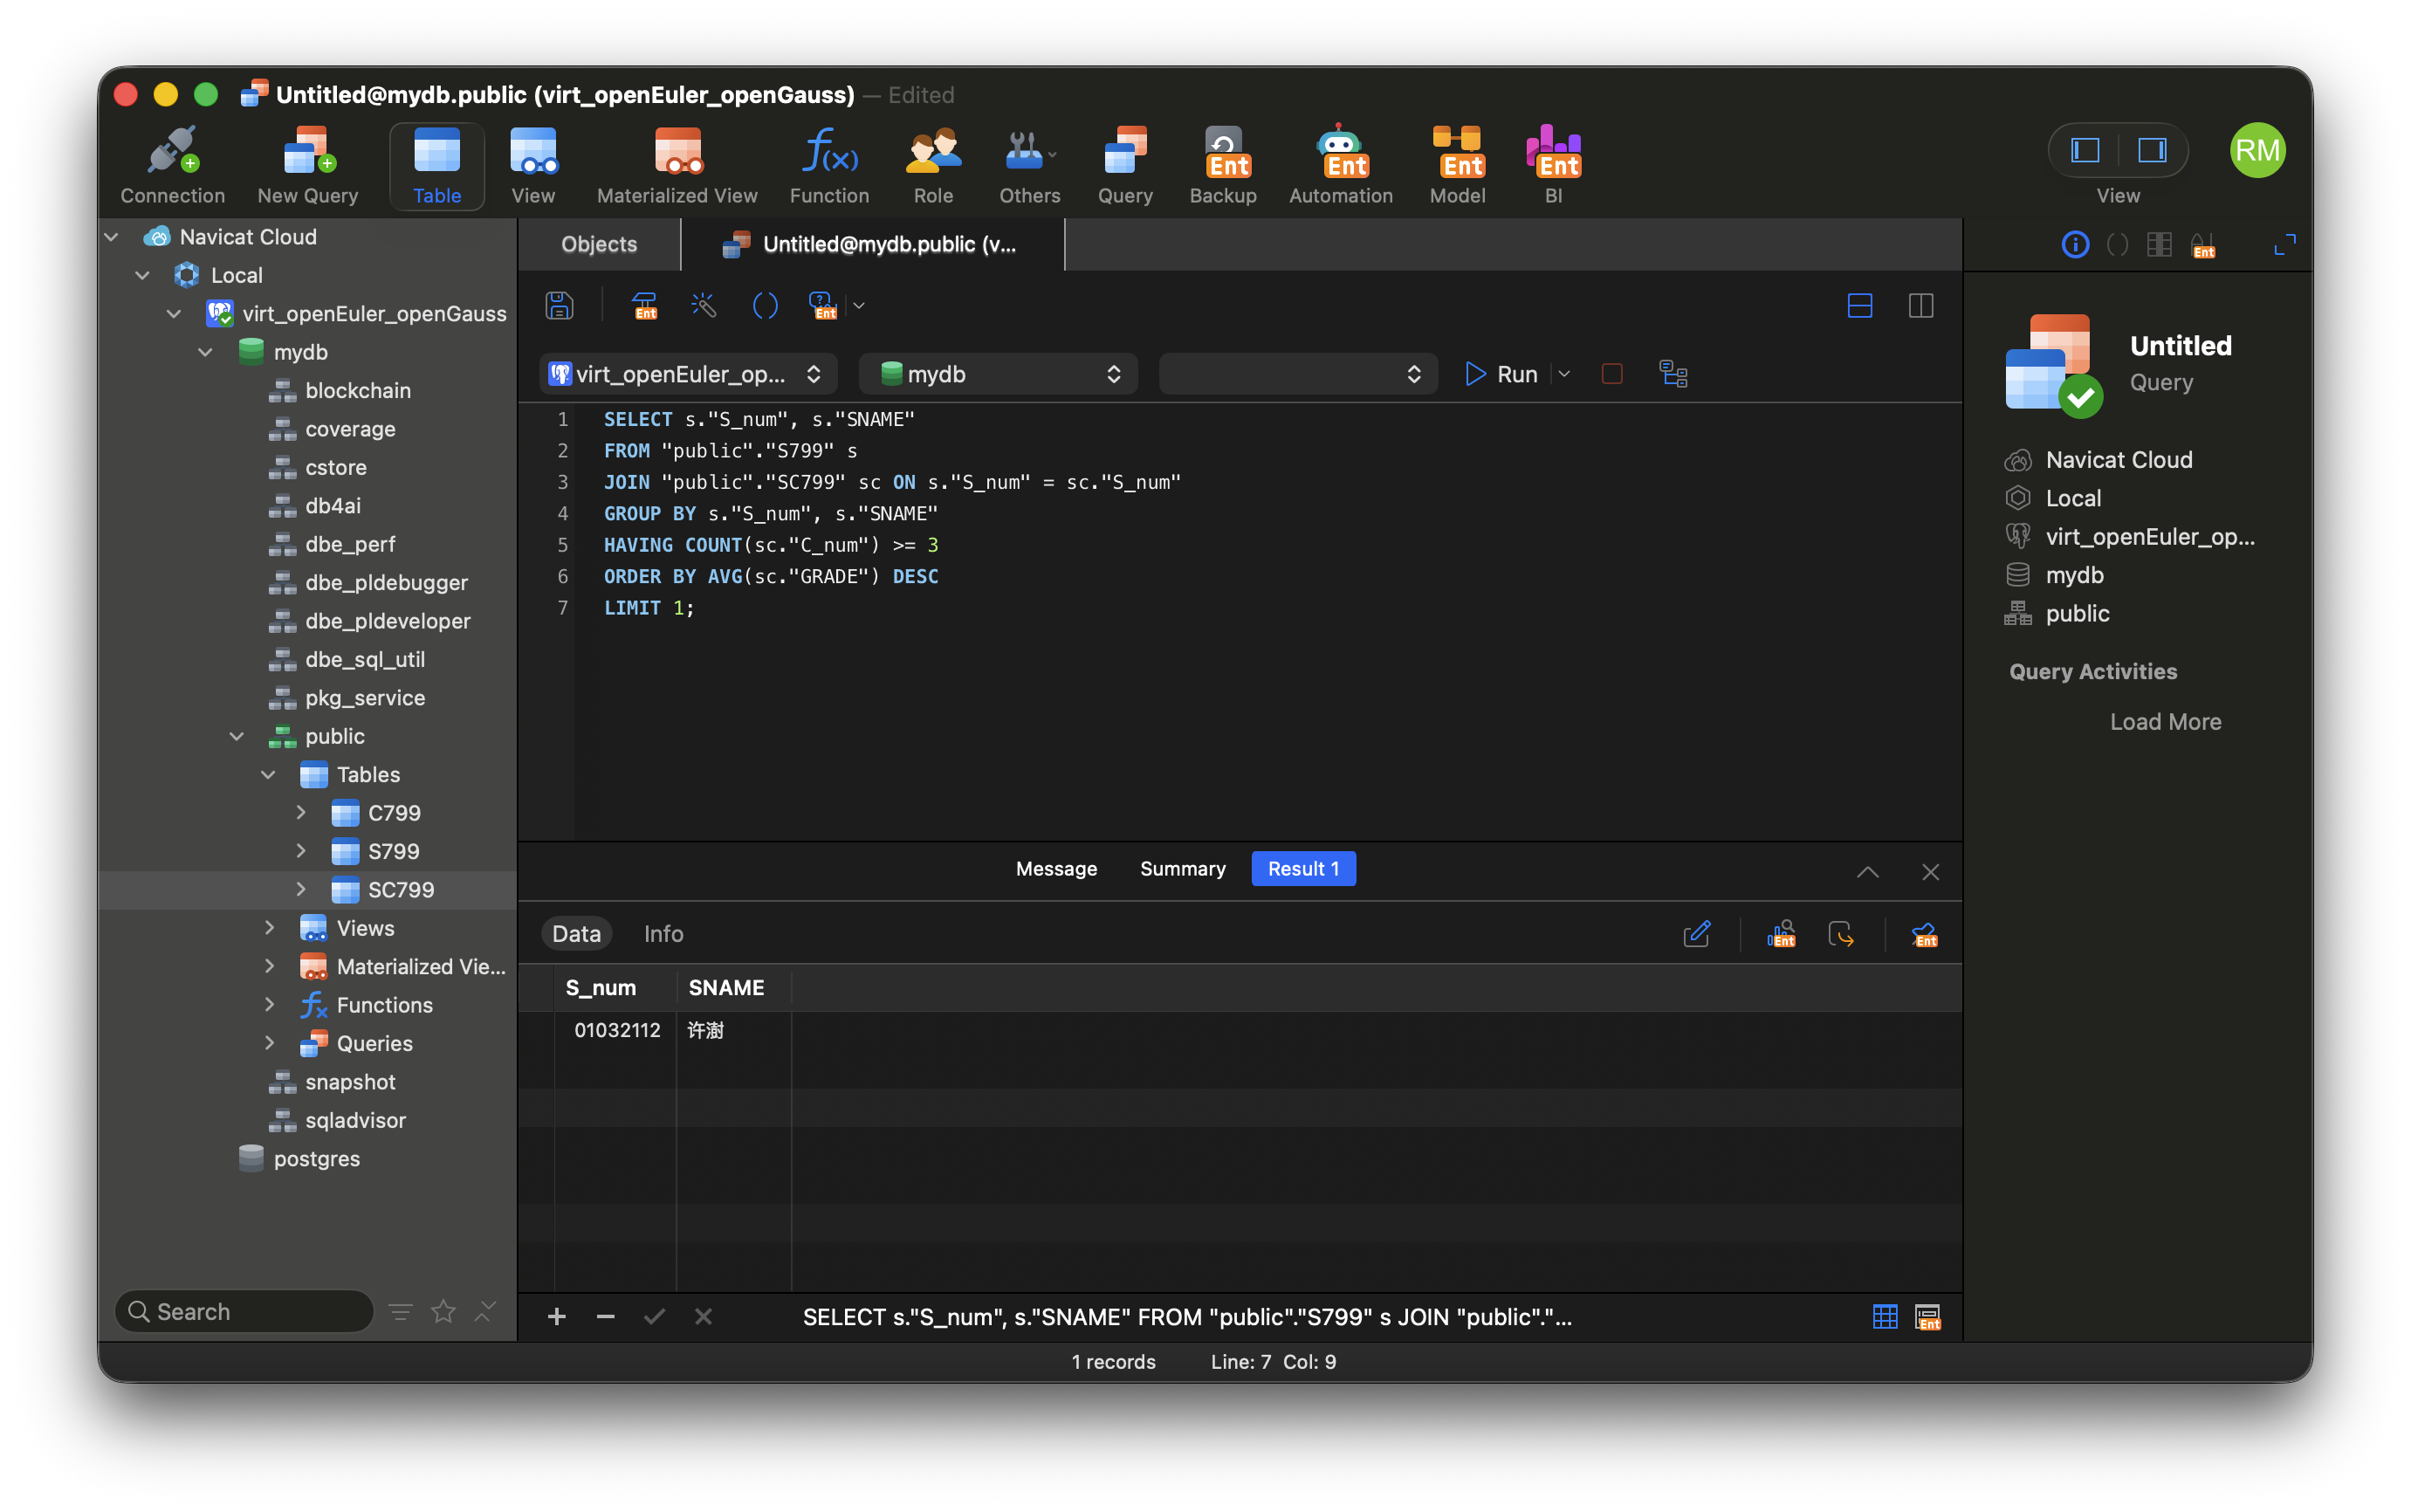
\includegraphics[width=0.88\textwidth]{images/14_3_1(8).png}
\caption{查询选修 3 门及以上课程中平均成绩最高的学生}
\label{fig:q8}
\end{figure}

选修 3 门及以上课程的学生包括王涛、张晓梅、刘静、孙文、许澍（CS 系学生均选 3 门以上）。其中许澍（CS-05 成绩为 NULL，不参与均值计算）在 CS-01、CS-02、CS-04 上均分约 88.5，位列第一。

\subsubsection{2. 插入新记录}

实验要求分别在 S799 和 C799 中插入以下记录：
\begin{itemize}
  \item S799：\texttt{('01032005', '刘竞', '男', '2003-12-10', 1.75, '东14舍312')}
  \item C799：\texttt{('CS-03', '离散数学', 64, 4, '陈建明')}
\end{itemize}

\textbf{主键冲突演示}：首先尝试将学号 \texttt{01032005} 的新记录插入 S799：

\begin{lstlisting}[style=sqlstyle]
INSERT INTO "public"."S799"
  ("S_num","SNAME","SEX","BDATE","HEIGHT","DORM")
VALUES ('01032005','刘竞','男','2003-12-10',1.75,'东14舍312');
\end{lstlisting}

\begin{figure}[H]
\centering
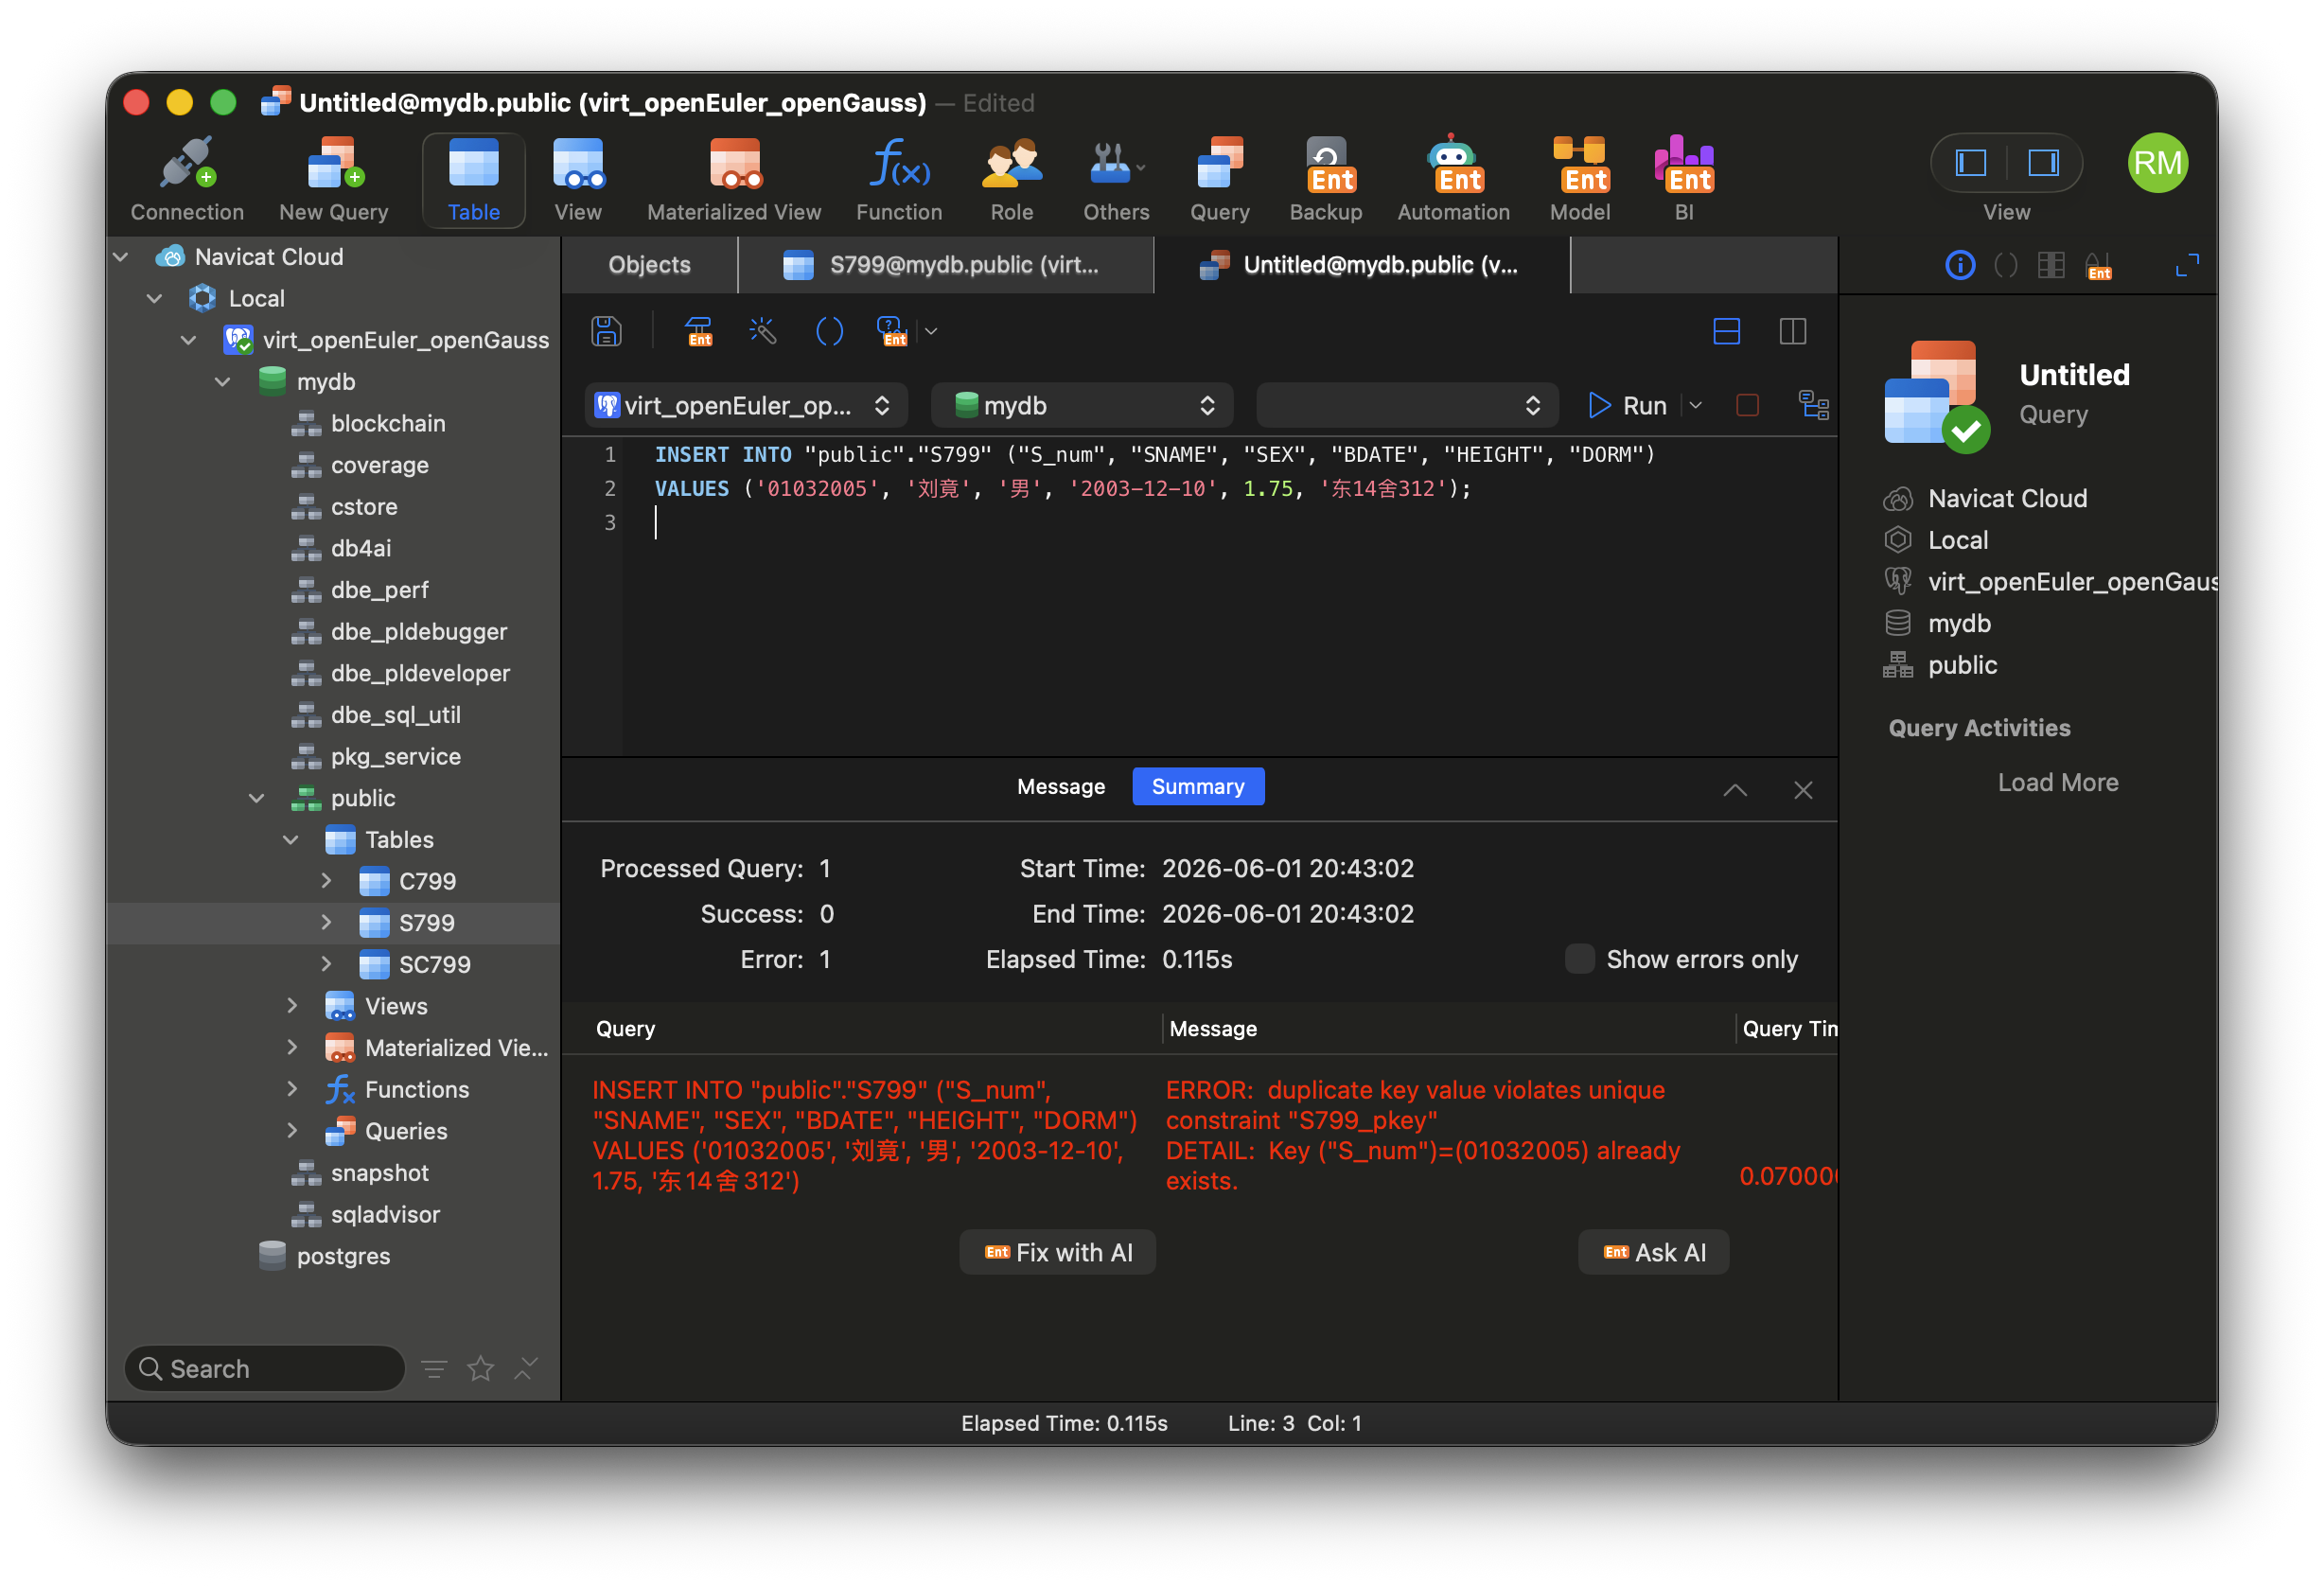
\includegraphics[width=0.88\textwidth]{images/15_3_2_1.png}
\caption{尝试插入学号 01032005 的新记录时出现主键重复冲突错误}
\label{fig:insert_conflict}
\end{figure}

数据库报告主键冲突错误，因为学号 \texttt{01032005} 在 S799 中已存在（对应学生刘静）。这正是主键约束保障\textbf{实体完整性}的体现：S799 中每个学生具有唯一学号，数据库拒绝重复学号的插入。

对于课程记录 CS-03 的插入，由于 C799 中尚不存在该课程编号，故不存在冲突，插入成功：

\begin{lstlisting}[style=sqlstyle]
INSERT INTO "public"."C799"
  ("C_num","CNAME","PERIOD","CREDIT","TEACHER")
VALUES ('CS-03','离散数学',64,4,'陈建明');
\end{lstlisting}

\begin{figure}[H]
\centering
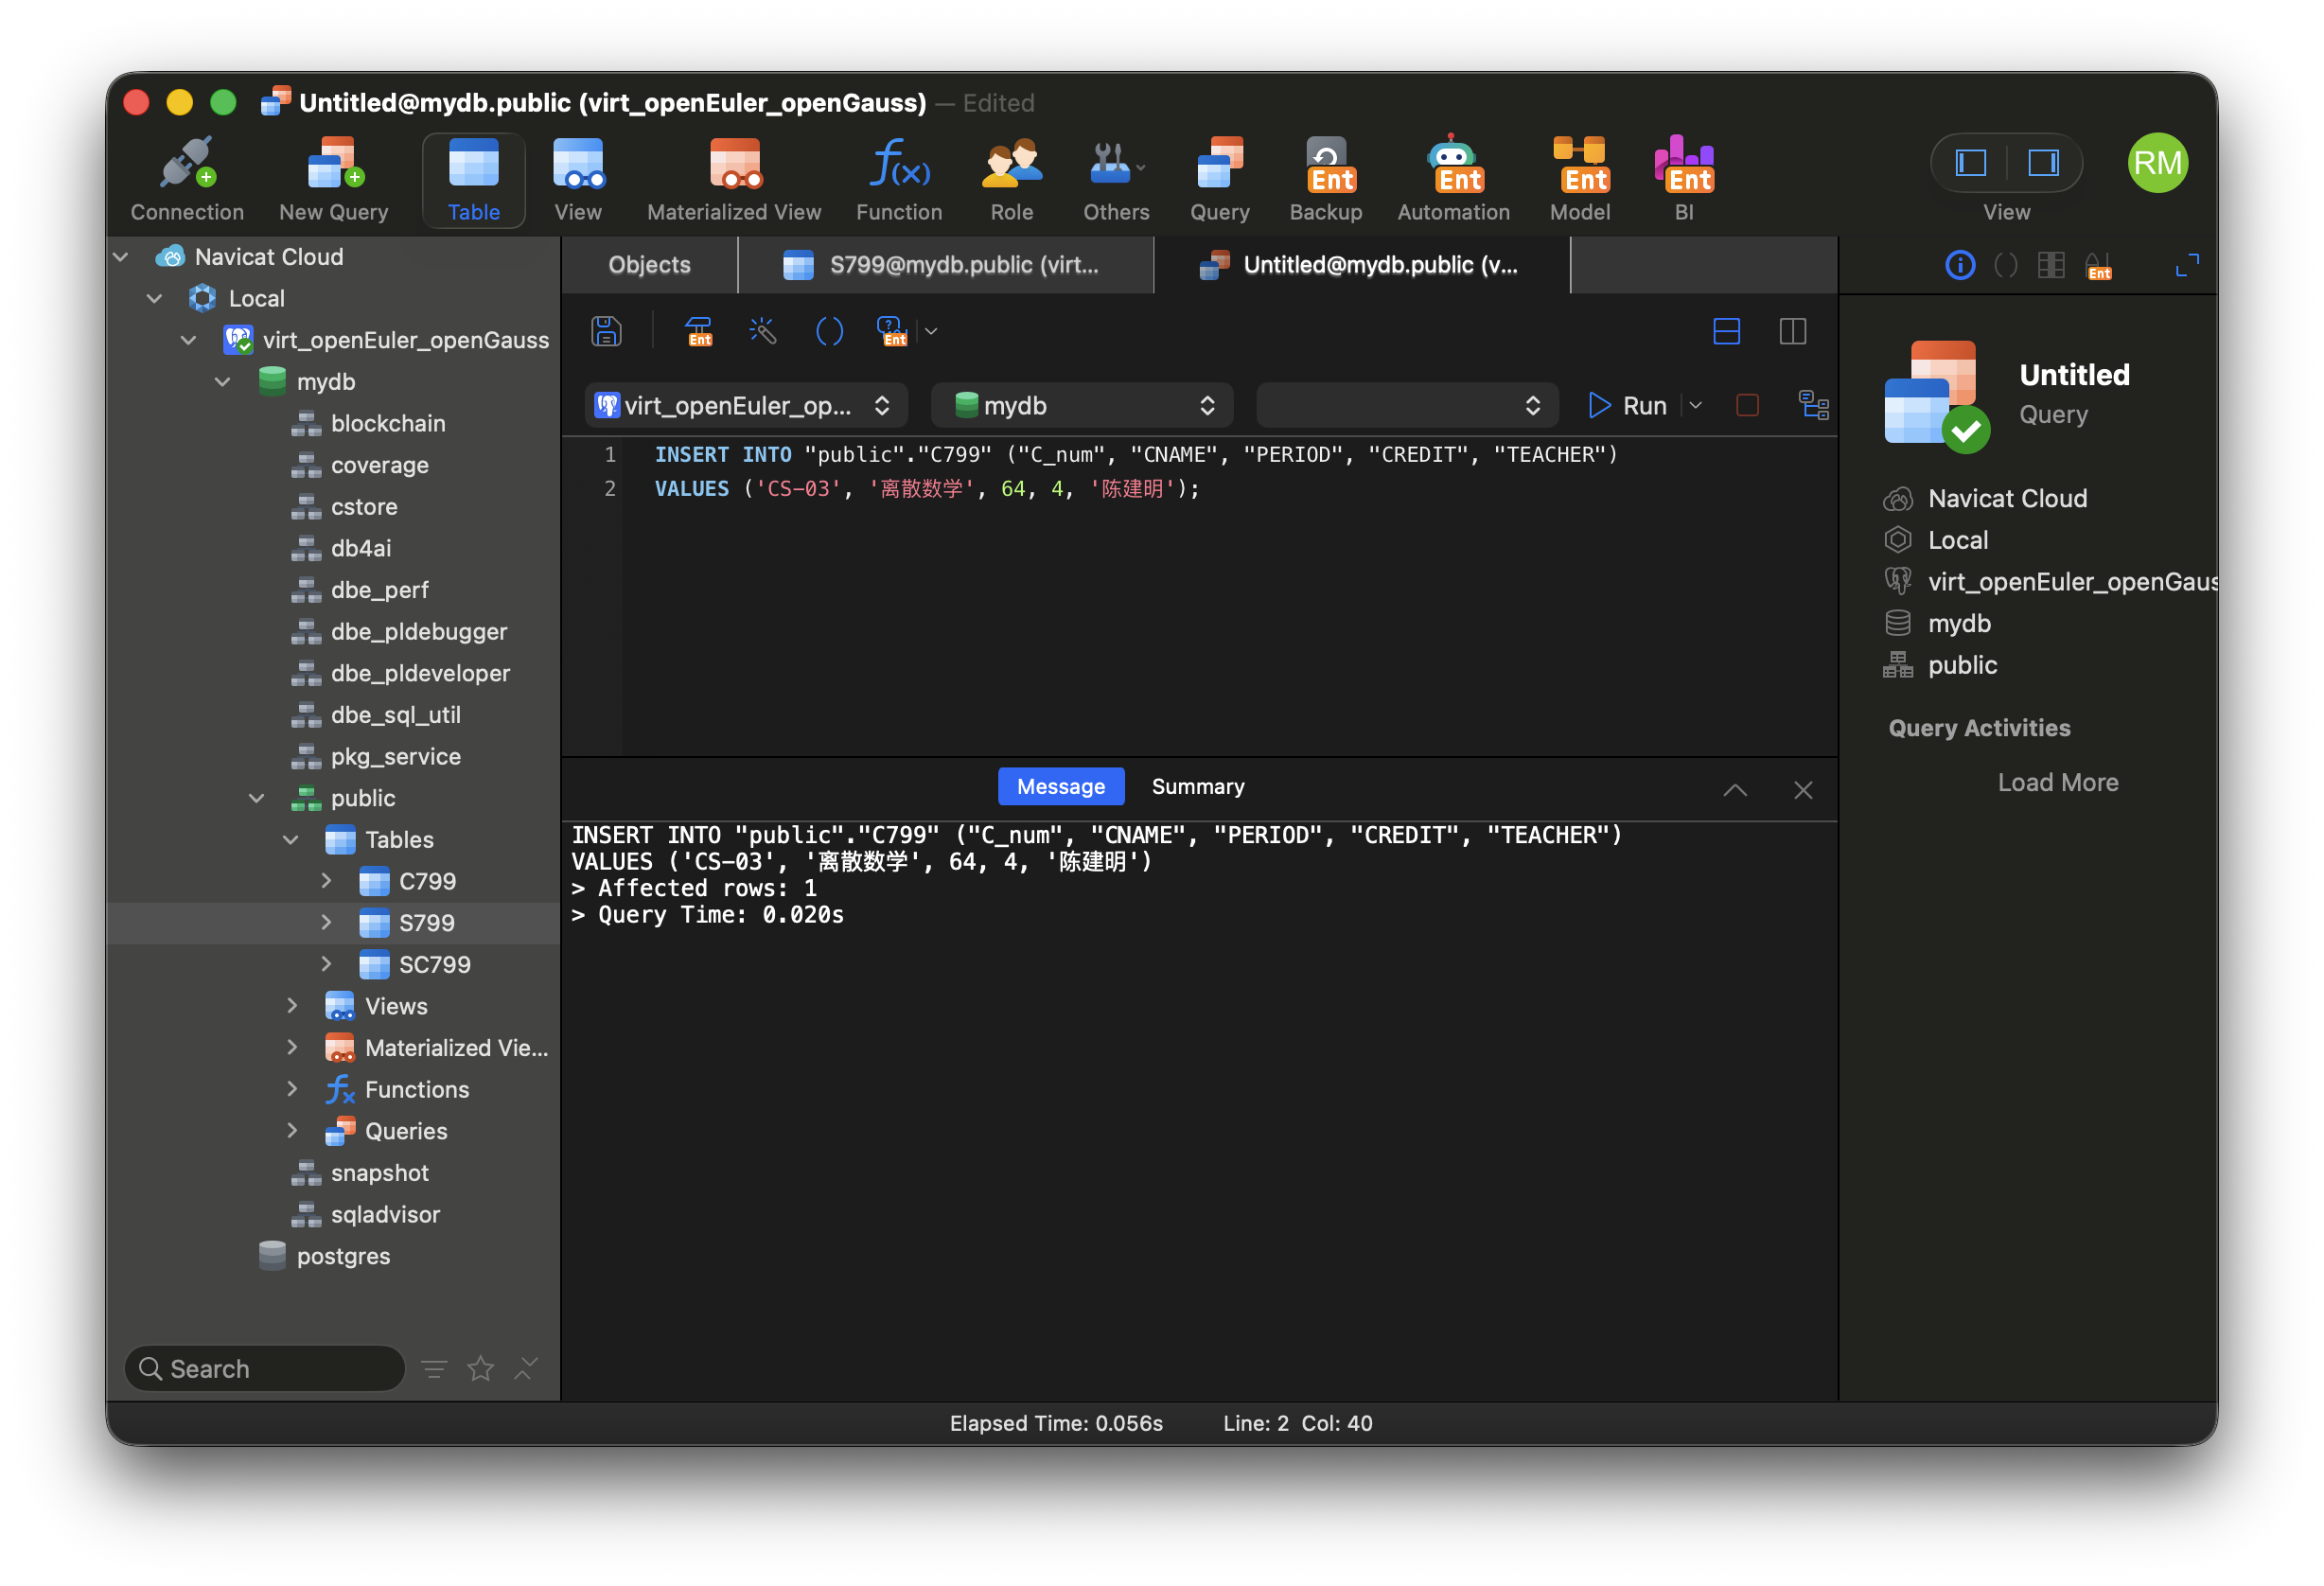
\includegraphics[width=0.88\textwidth]{images/16_3_2_2.png}
\caption{成功向 C799 插入课程 CS-03（离散数学，64 学时，4 学分，陈建明老师）}
\label{fig:insert_success}
\end{figure}

课程 CS-03（离散数学）成功加入 C799，学时 64，学分 4，教师陈建明。至此 C799 共有 8 门课程（含原有 7 门）。

\subsubsection{3. 删除已修学分超过 20 的学生记录}

\textbf{思路}：通过 JOIN SC799 和 C799 计算每位学生的已选课程学分之和，筛选出总学分大于 20 的学号集合，再从 S799 中删除对应的学生记录。

\begin{lstlisting}[style=sqlstyle]
DELETE FROM "public"."S799"
WHERE "S_num" IN (
    SELECT sc."S_num"
    FROM "public"."SC799" sc
    JOIN "public"."C799" c ON sc."C_num" = c."C_num"
    GROUP BY sc."S_num"
    HAVING SUM(c."CREDIT") > 20
);
\end{lstlisting}

\begin{figure}[H]
\centering
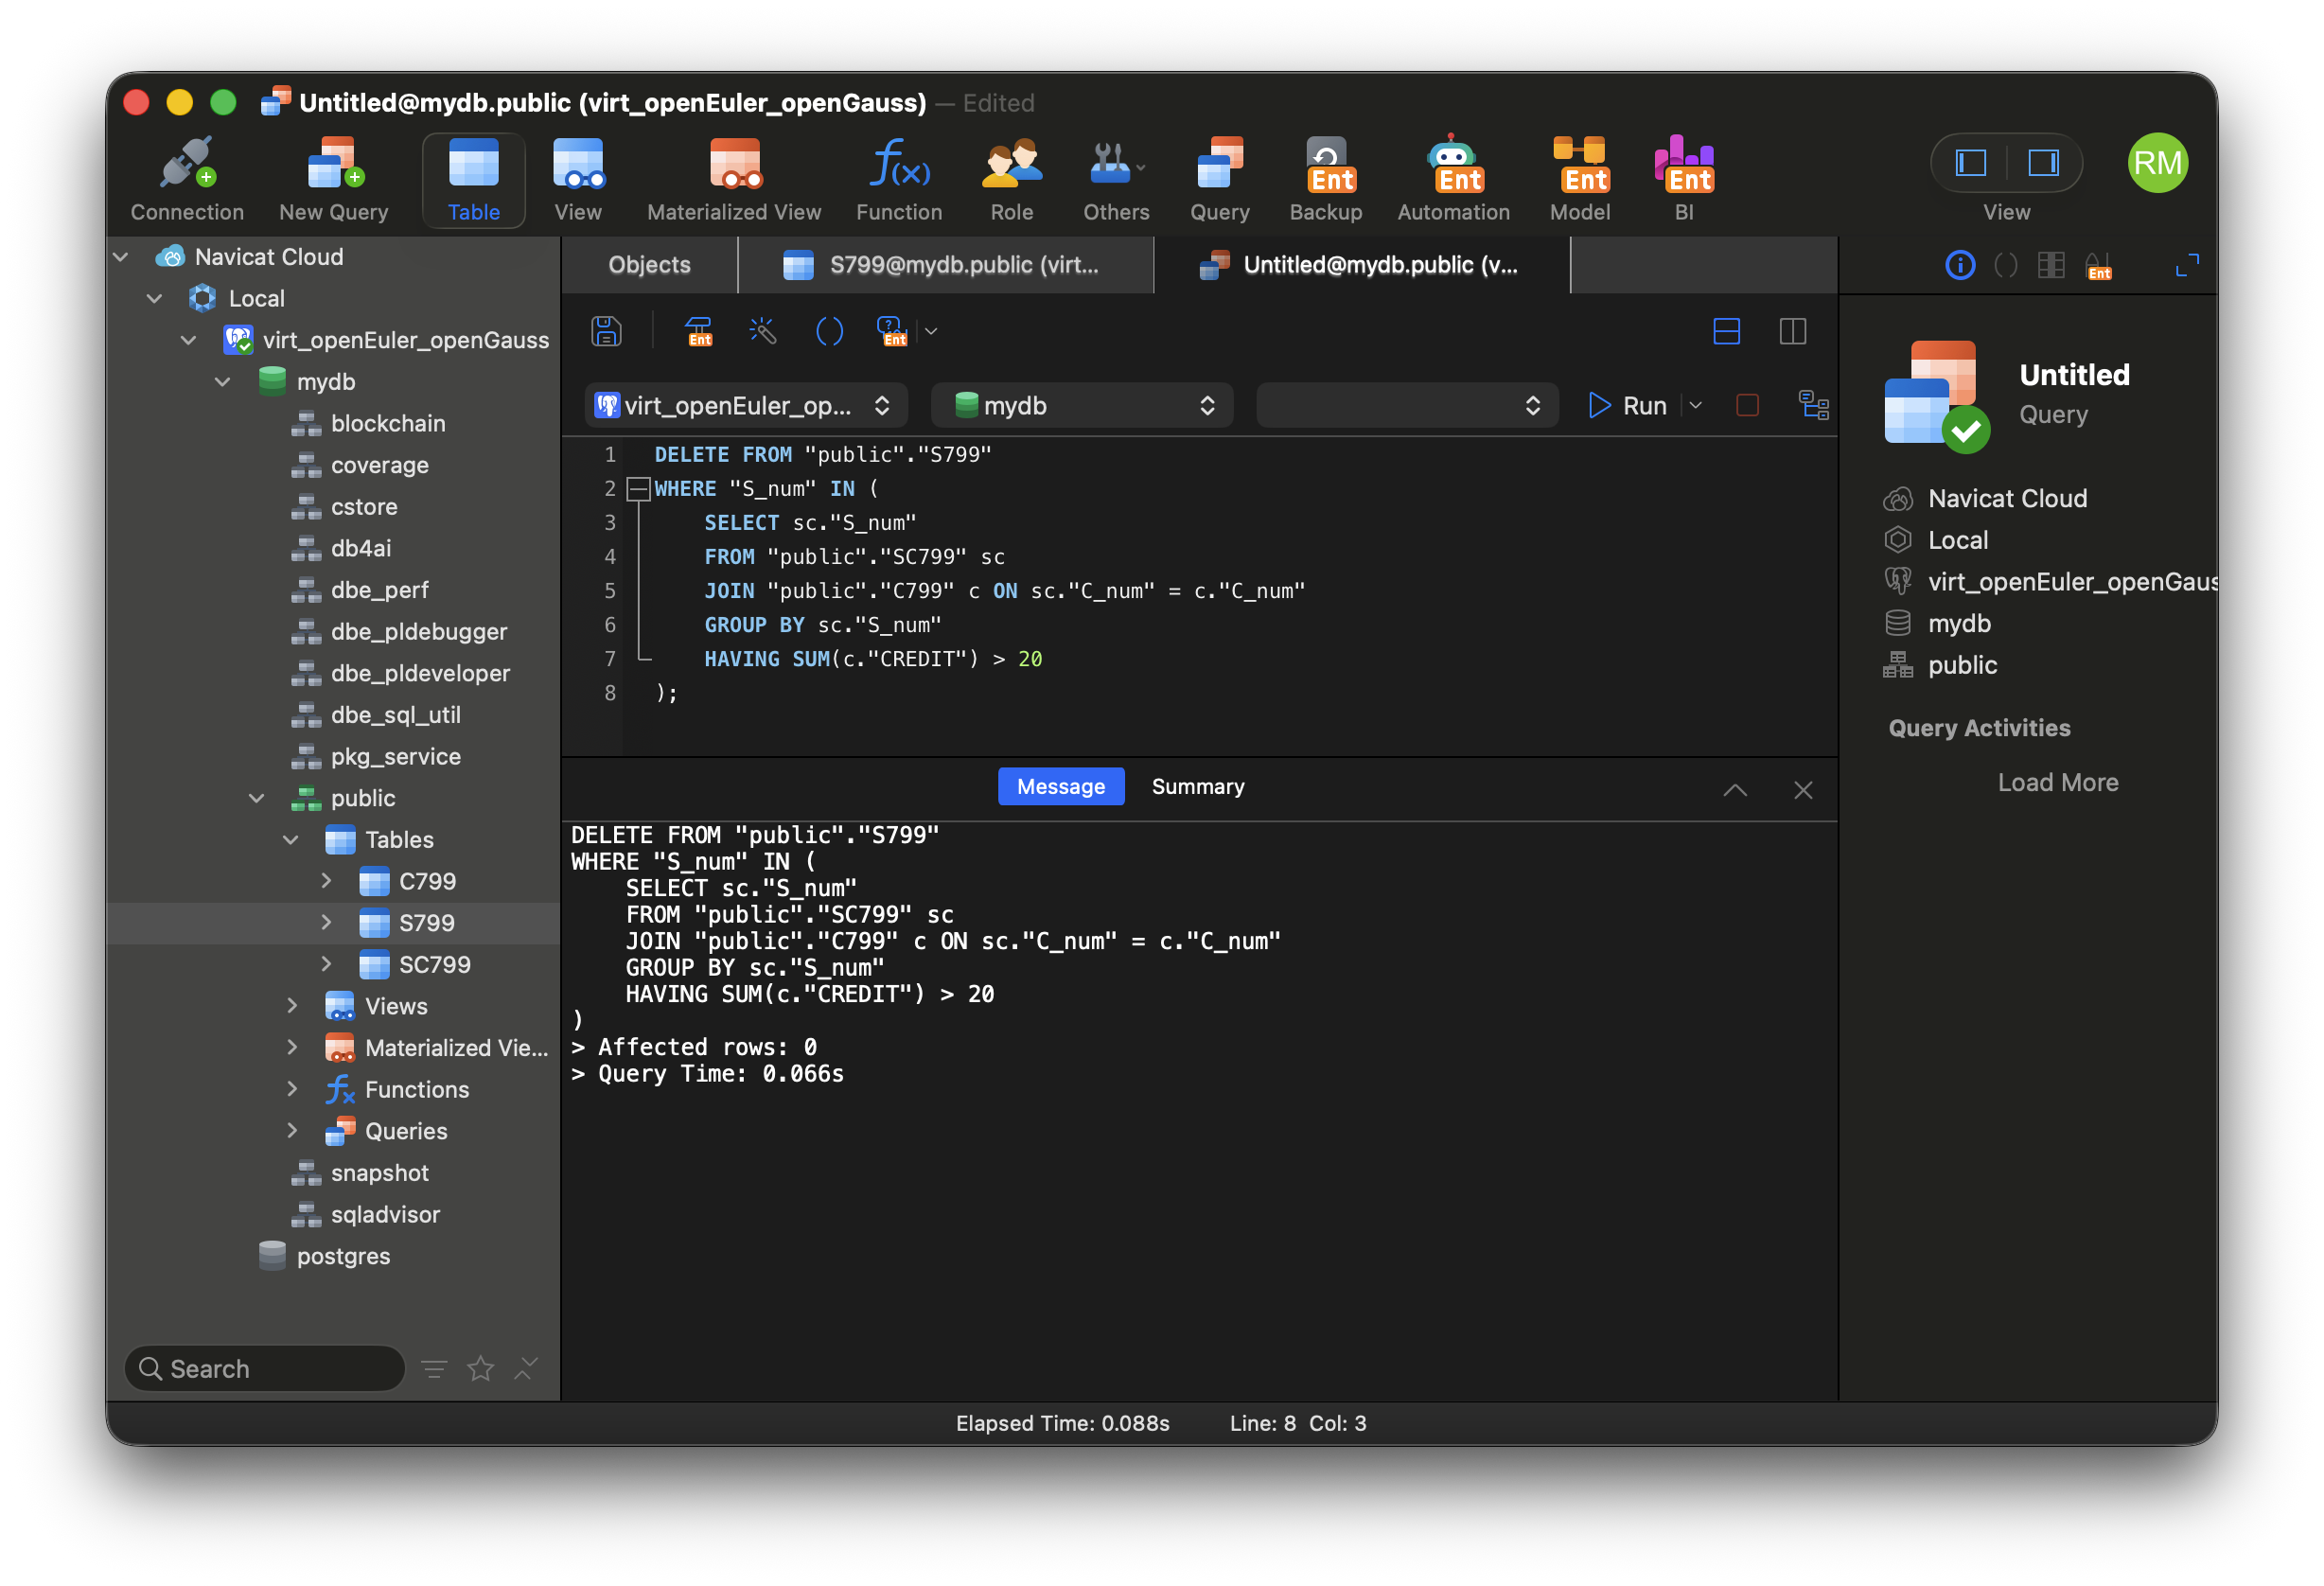
\includegraphics[width=0.88\textwidth]{images/17_3_3.png}
\caption{执行删除已修学分超过 20 的学生记录（影响行数为 0）}
\label{fig:delete}
\end{figure}

\textbf{结果分析}：在当前初始数据中，所有学生的选课学分总和均未超过 20（选课最多的许澍：$3+4+2+2=11$ 分，其余学生更少），因此子查询返回空集，DELETE 语句影响行数为 0，表数据未发生变化。这是符合预期的正确结果——SQL 语句逻辑正确，只是当前数据不满足删除条件。

\subsubsection{4. 更新课程信息}

\textbf{任务}：将"张明"老师负责的"数字电子技术"课程的学时数调整为 36，同时增加 1 个学分。

\begin{lstlisting}[style=sqlstyle]
UPDATE "public"."C799"
SET "PERIOD" = 36,
    "CREDIT" = "CREDIT" + 1
WHERE "TEACHER" = '张明'
  AND "CNAME"   = '数字电子技术';
\end{lstlisting}

\begin{figure}[H]
\centering
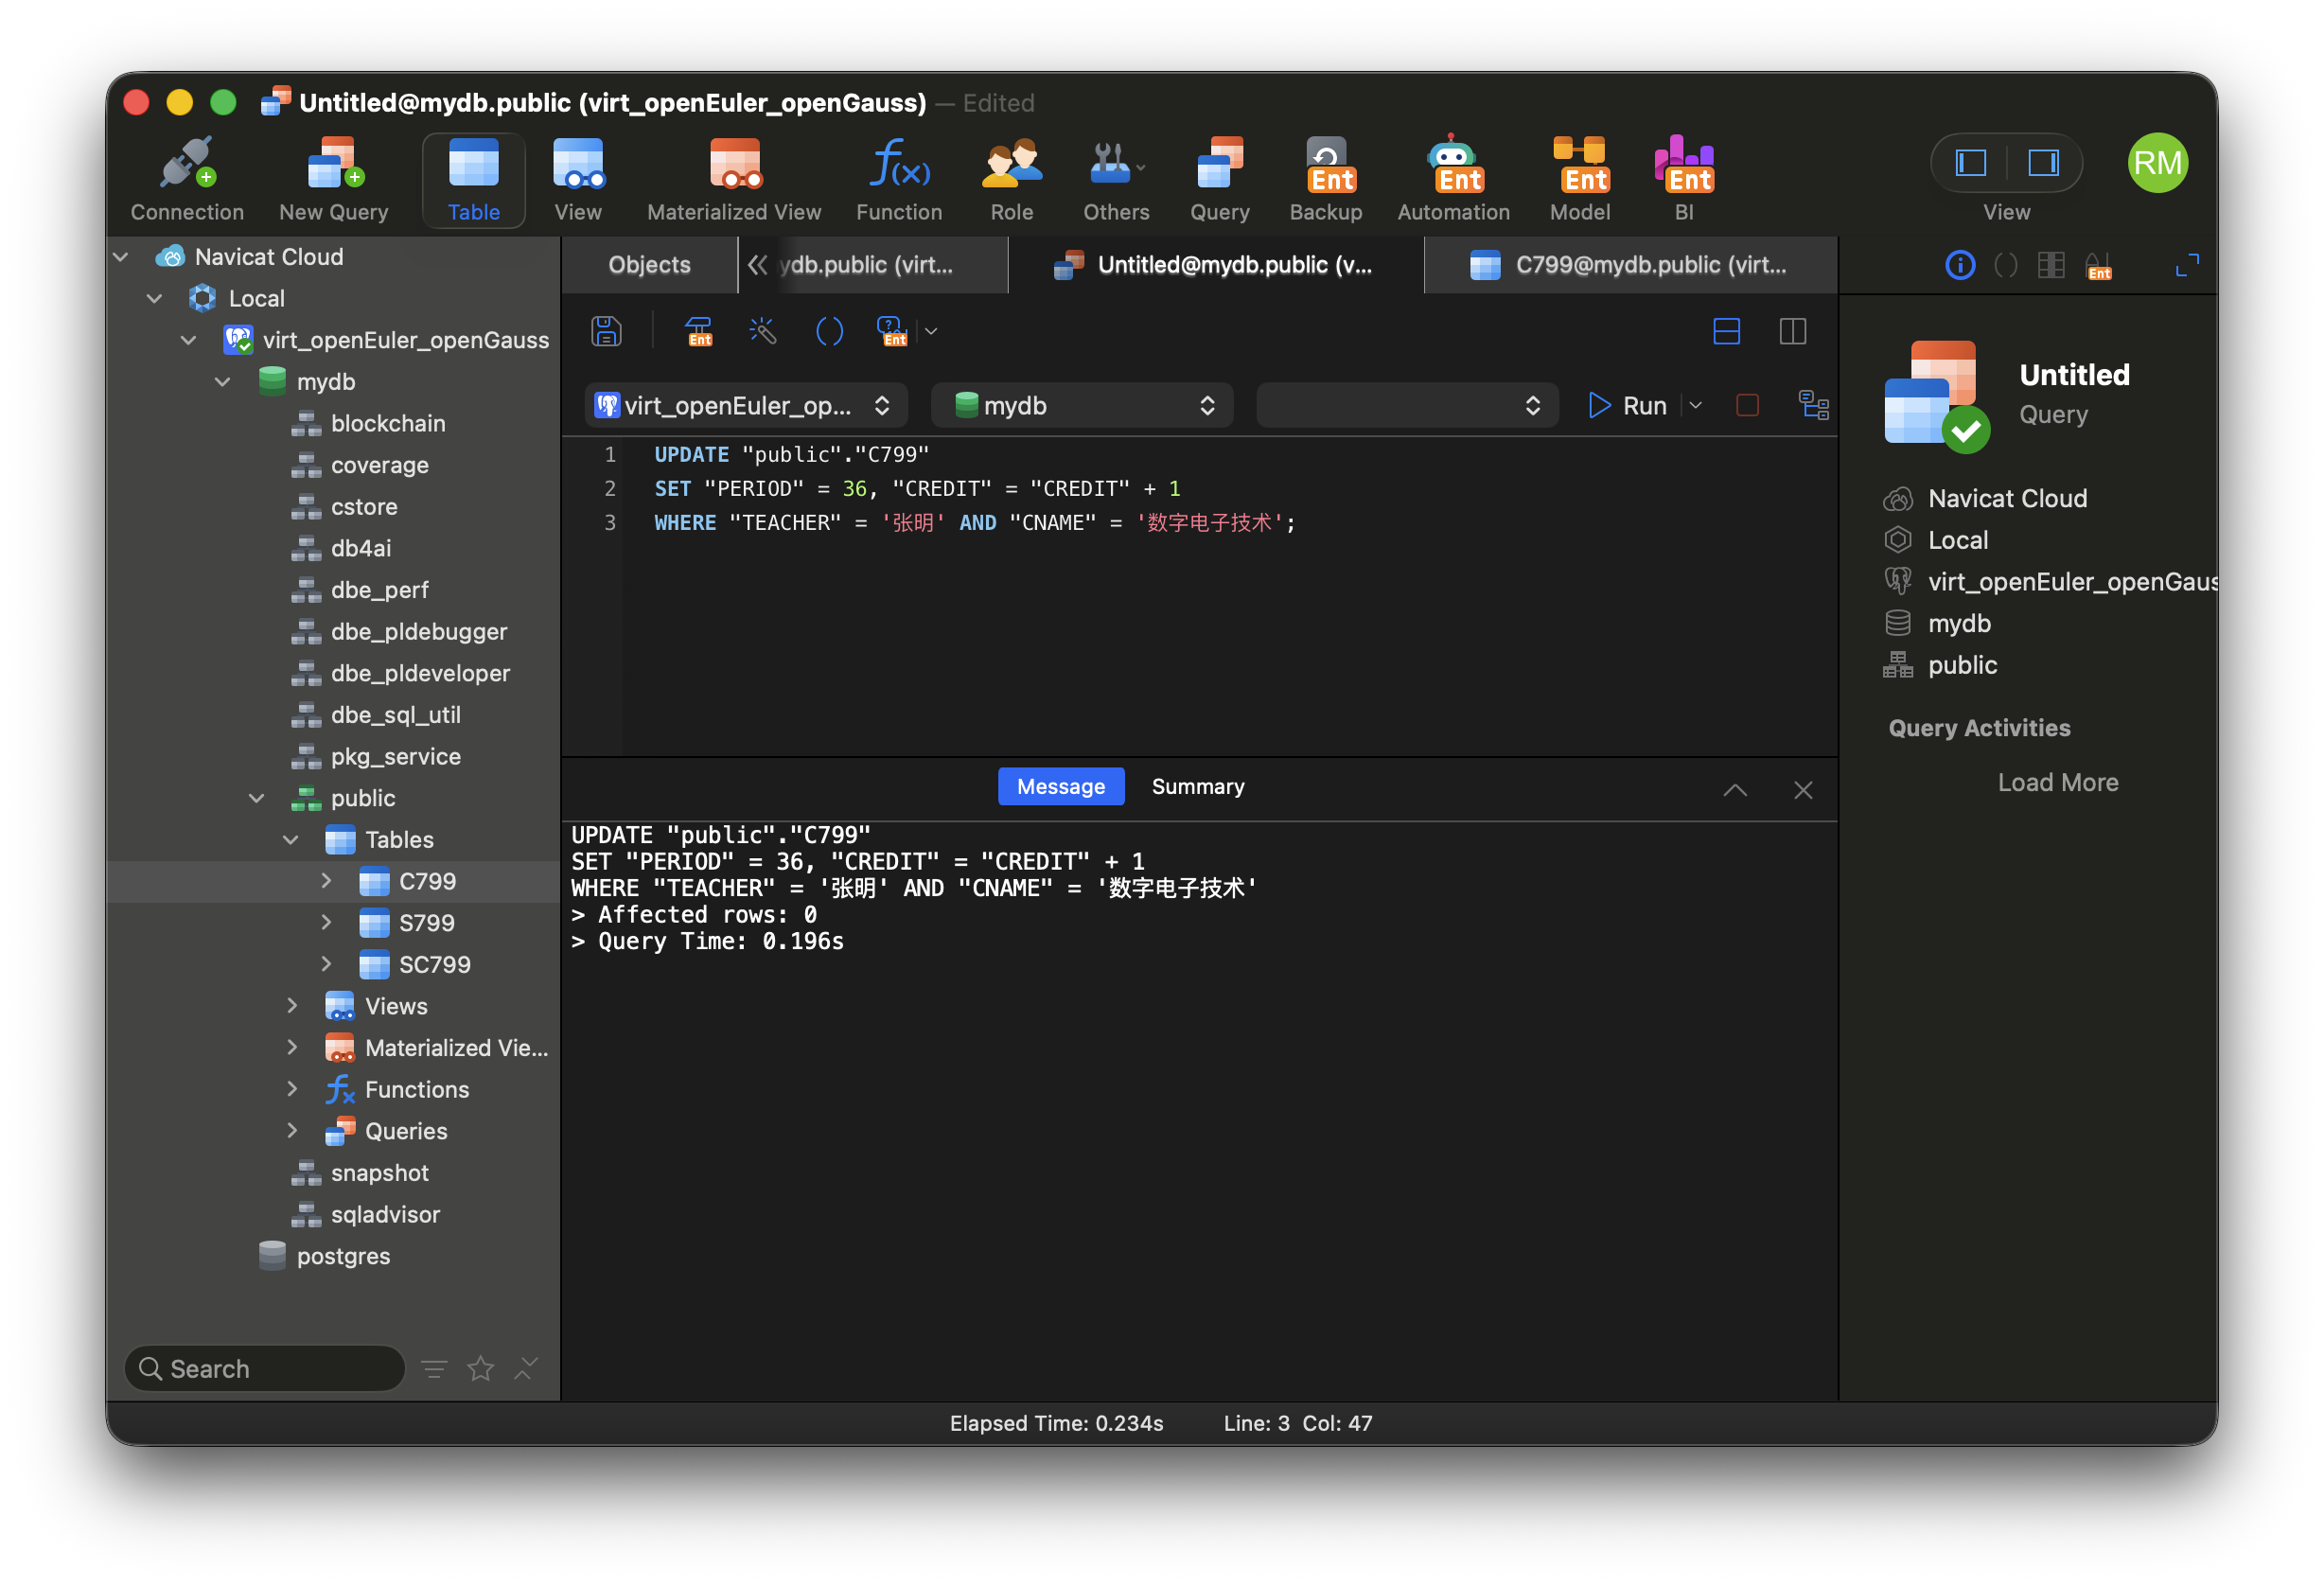
\includegraphics[width=0.88\textwidth]{images/18_3_4.png}
\caption{执行课程信息更新操作（影响行数为 0）}
\label{fig:update}
\end{figure}

\textbf{结果分析}：当前 C799 中张明老师负责的课程为"信号与系统"（EE-01），数据库中并不存在课程名为"数字电子技术"的记录，因此 \texttt{WHERE} 子句无法匹配任何行，UPDATE 语句影响行数为 0，表数据未变化。关系数据库在无匹配条件时会安全地完成操作而不修改任何数据，这也体现了 SQL 操作的幂等安全性。

\subsubsection{5. 创建视图}

\paragraph{(1) 居住在"东18舍"的男生视图}

创建包含住宿在东18舍的全部男生信息的视图，使用 \texttt{LIKE '东18舍\%'} 对宿舍字段进行前缀匹配：

\begin{lstlisting}[style=sqlstyle]
CREATE VIEW "view_male_dorm18" AS
SELECT "S_num","SNAME","BDATE","HEIGHT","SEX","DORM"
FROM "public"."S799"
WHERE "SEX" = '男' AND "DORM" LIKE '东18舍%';
\end{lstlisting}

\begin{figure}[H]
\centering
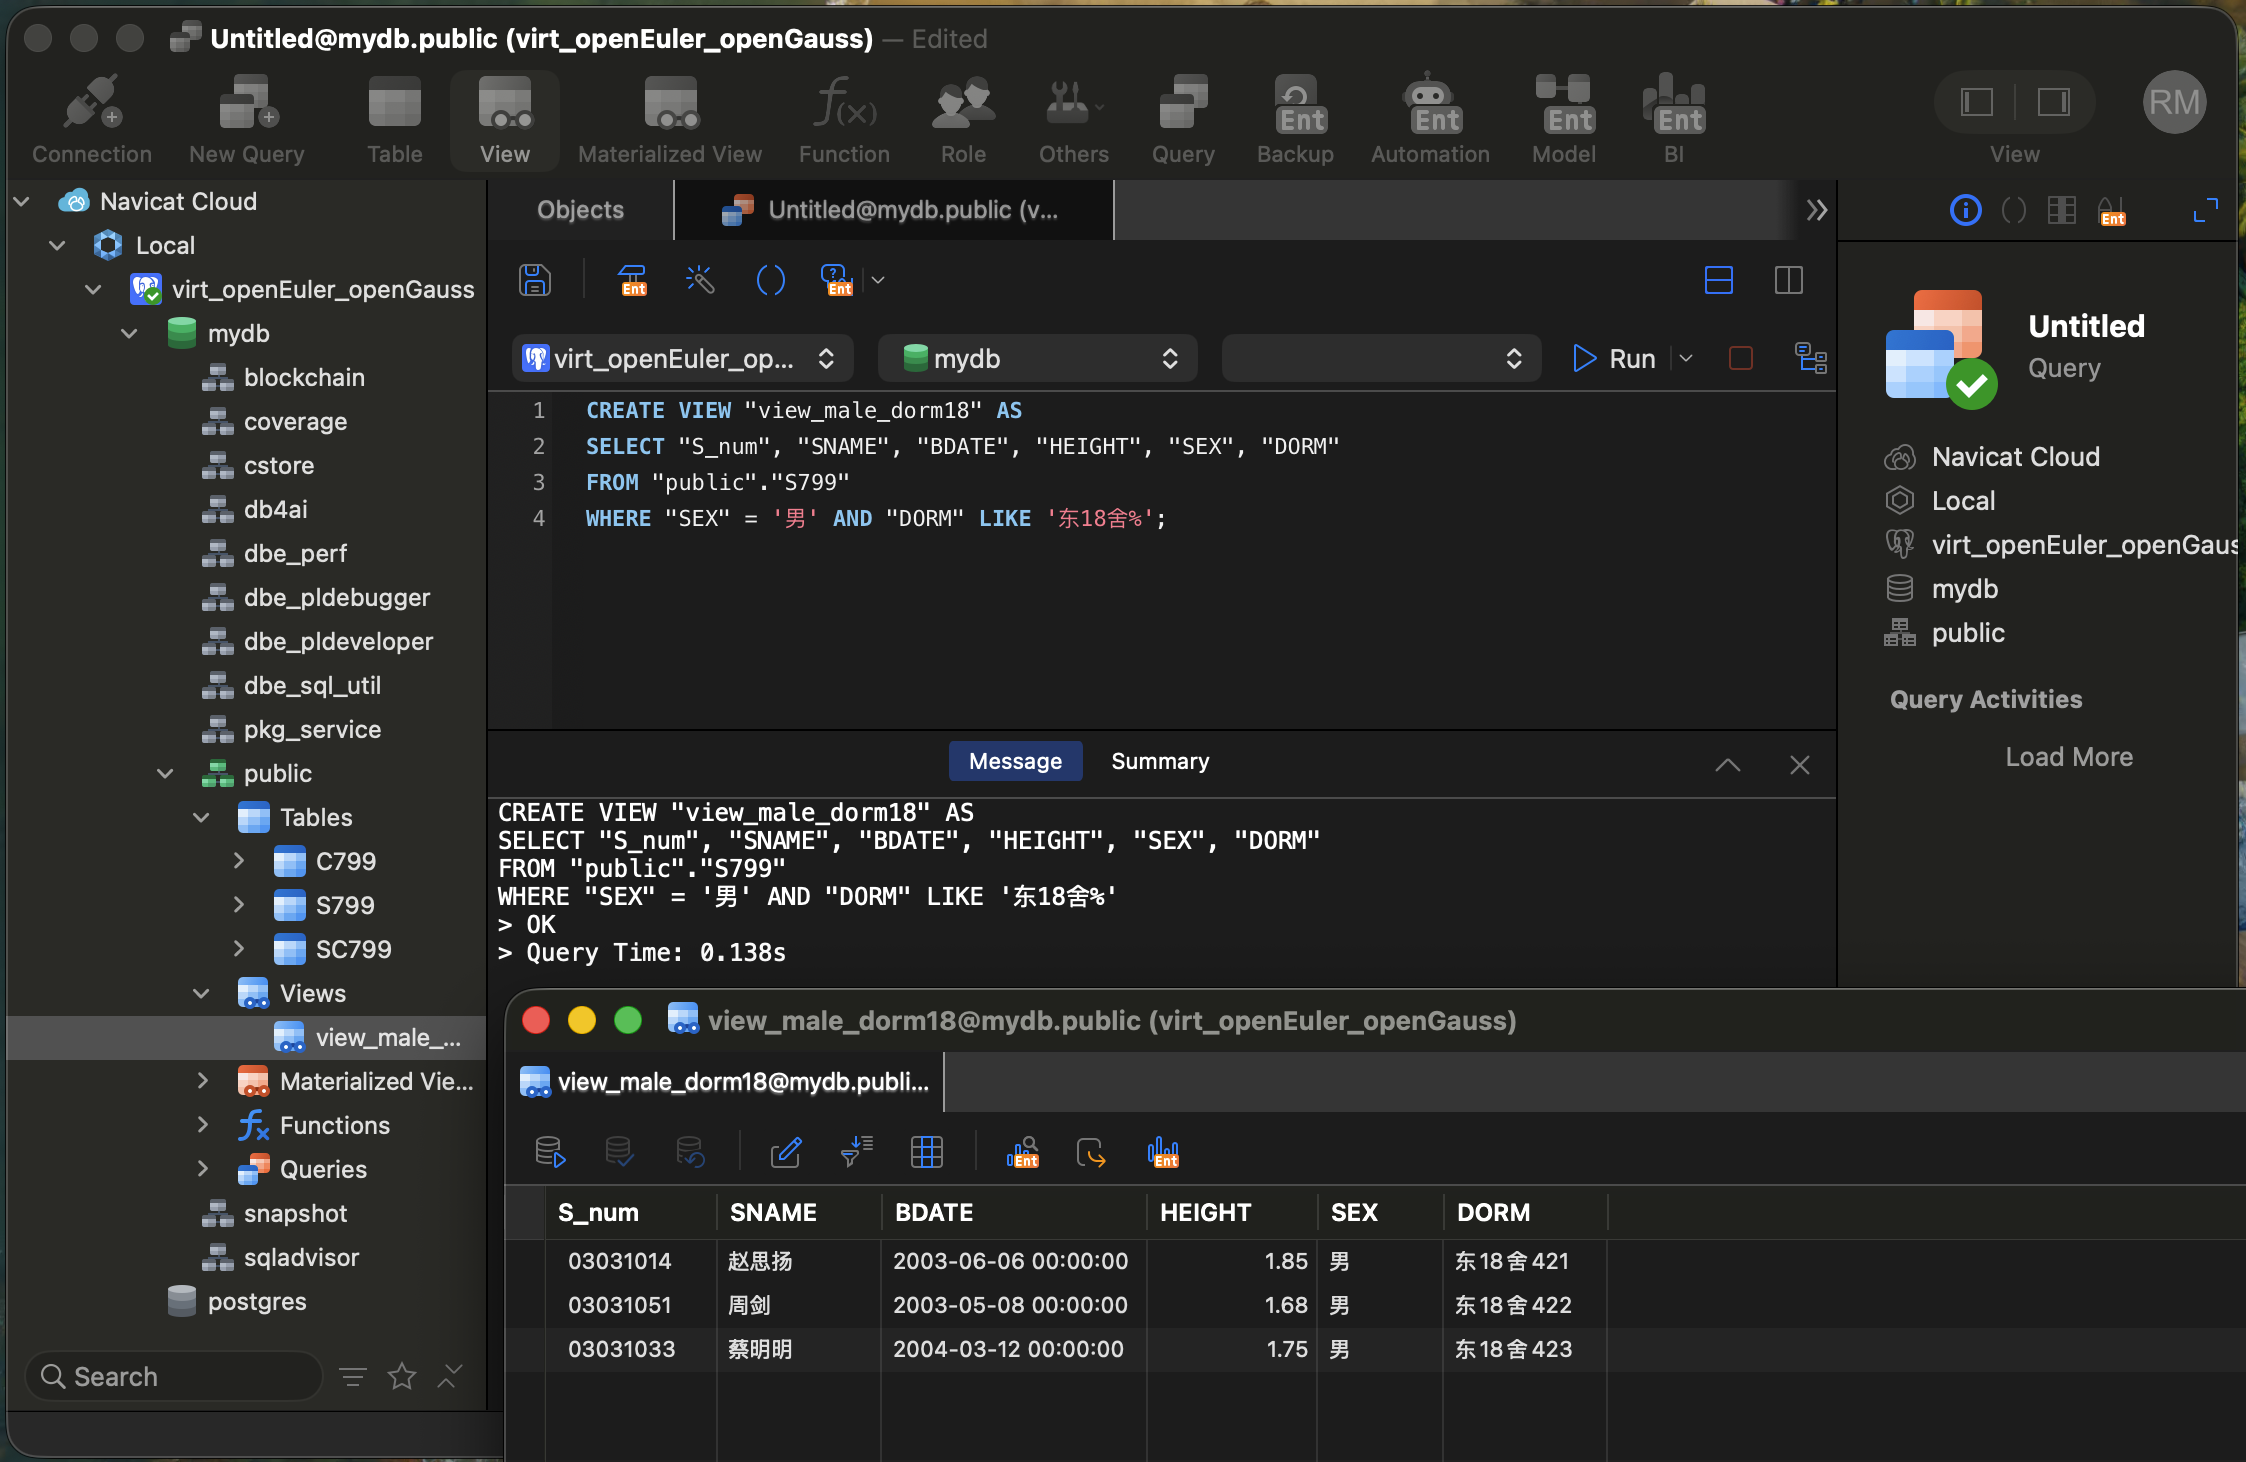
\includegraphics[width=0.88\textwidth]{images/19_3_5(1).png}
\caption{创建视图 view\_male\_dorm18：居住在东18舍的男生基本信息}
\label{fig:view1}
\end{figure}

视图内容包含赵思扬（东18舍421）、周剑（东18舍422）、蔡明明（东18舍423）三位男生。视图本质上是一个命名的虚拟表，每次查询视图时数据库重新执行底层 SQL，保证数据实时性。

\paragraph{(2) "张明"老师所开设课程情况的视图（含平均成绩）}

该视图展示张明老师负责的全部课程及其平均成绩，使用 \texttt{LEFT JOIN} 确保即使没有学生选课，该课程也会出现在视图中（平均成绩为 NULL）：

\begin{lstlisting}[style=sqlstyle]
CREATE VIEW "view_teacher_zhang_courses" AS
SELECT c."C_num", c."CNAME",
       AVG(sc."GRADE") AS "AVG_GRADE"
FROM "public"."C799" c
LEFT JOIN "public"."SC799" sc ON c."C_num" = sc."C_num"
WHERE c."TEACHER" = '张明'
GROUP BY c."C_num", c."CNAME";
\end{lstlisting}

\begin{figure}[H]
\centering
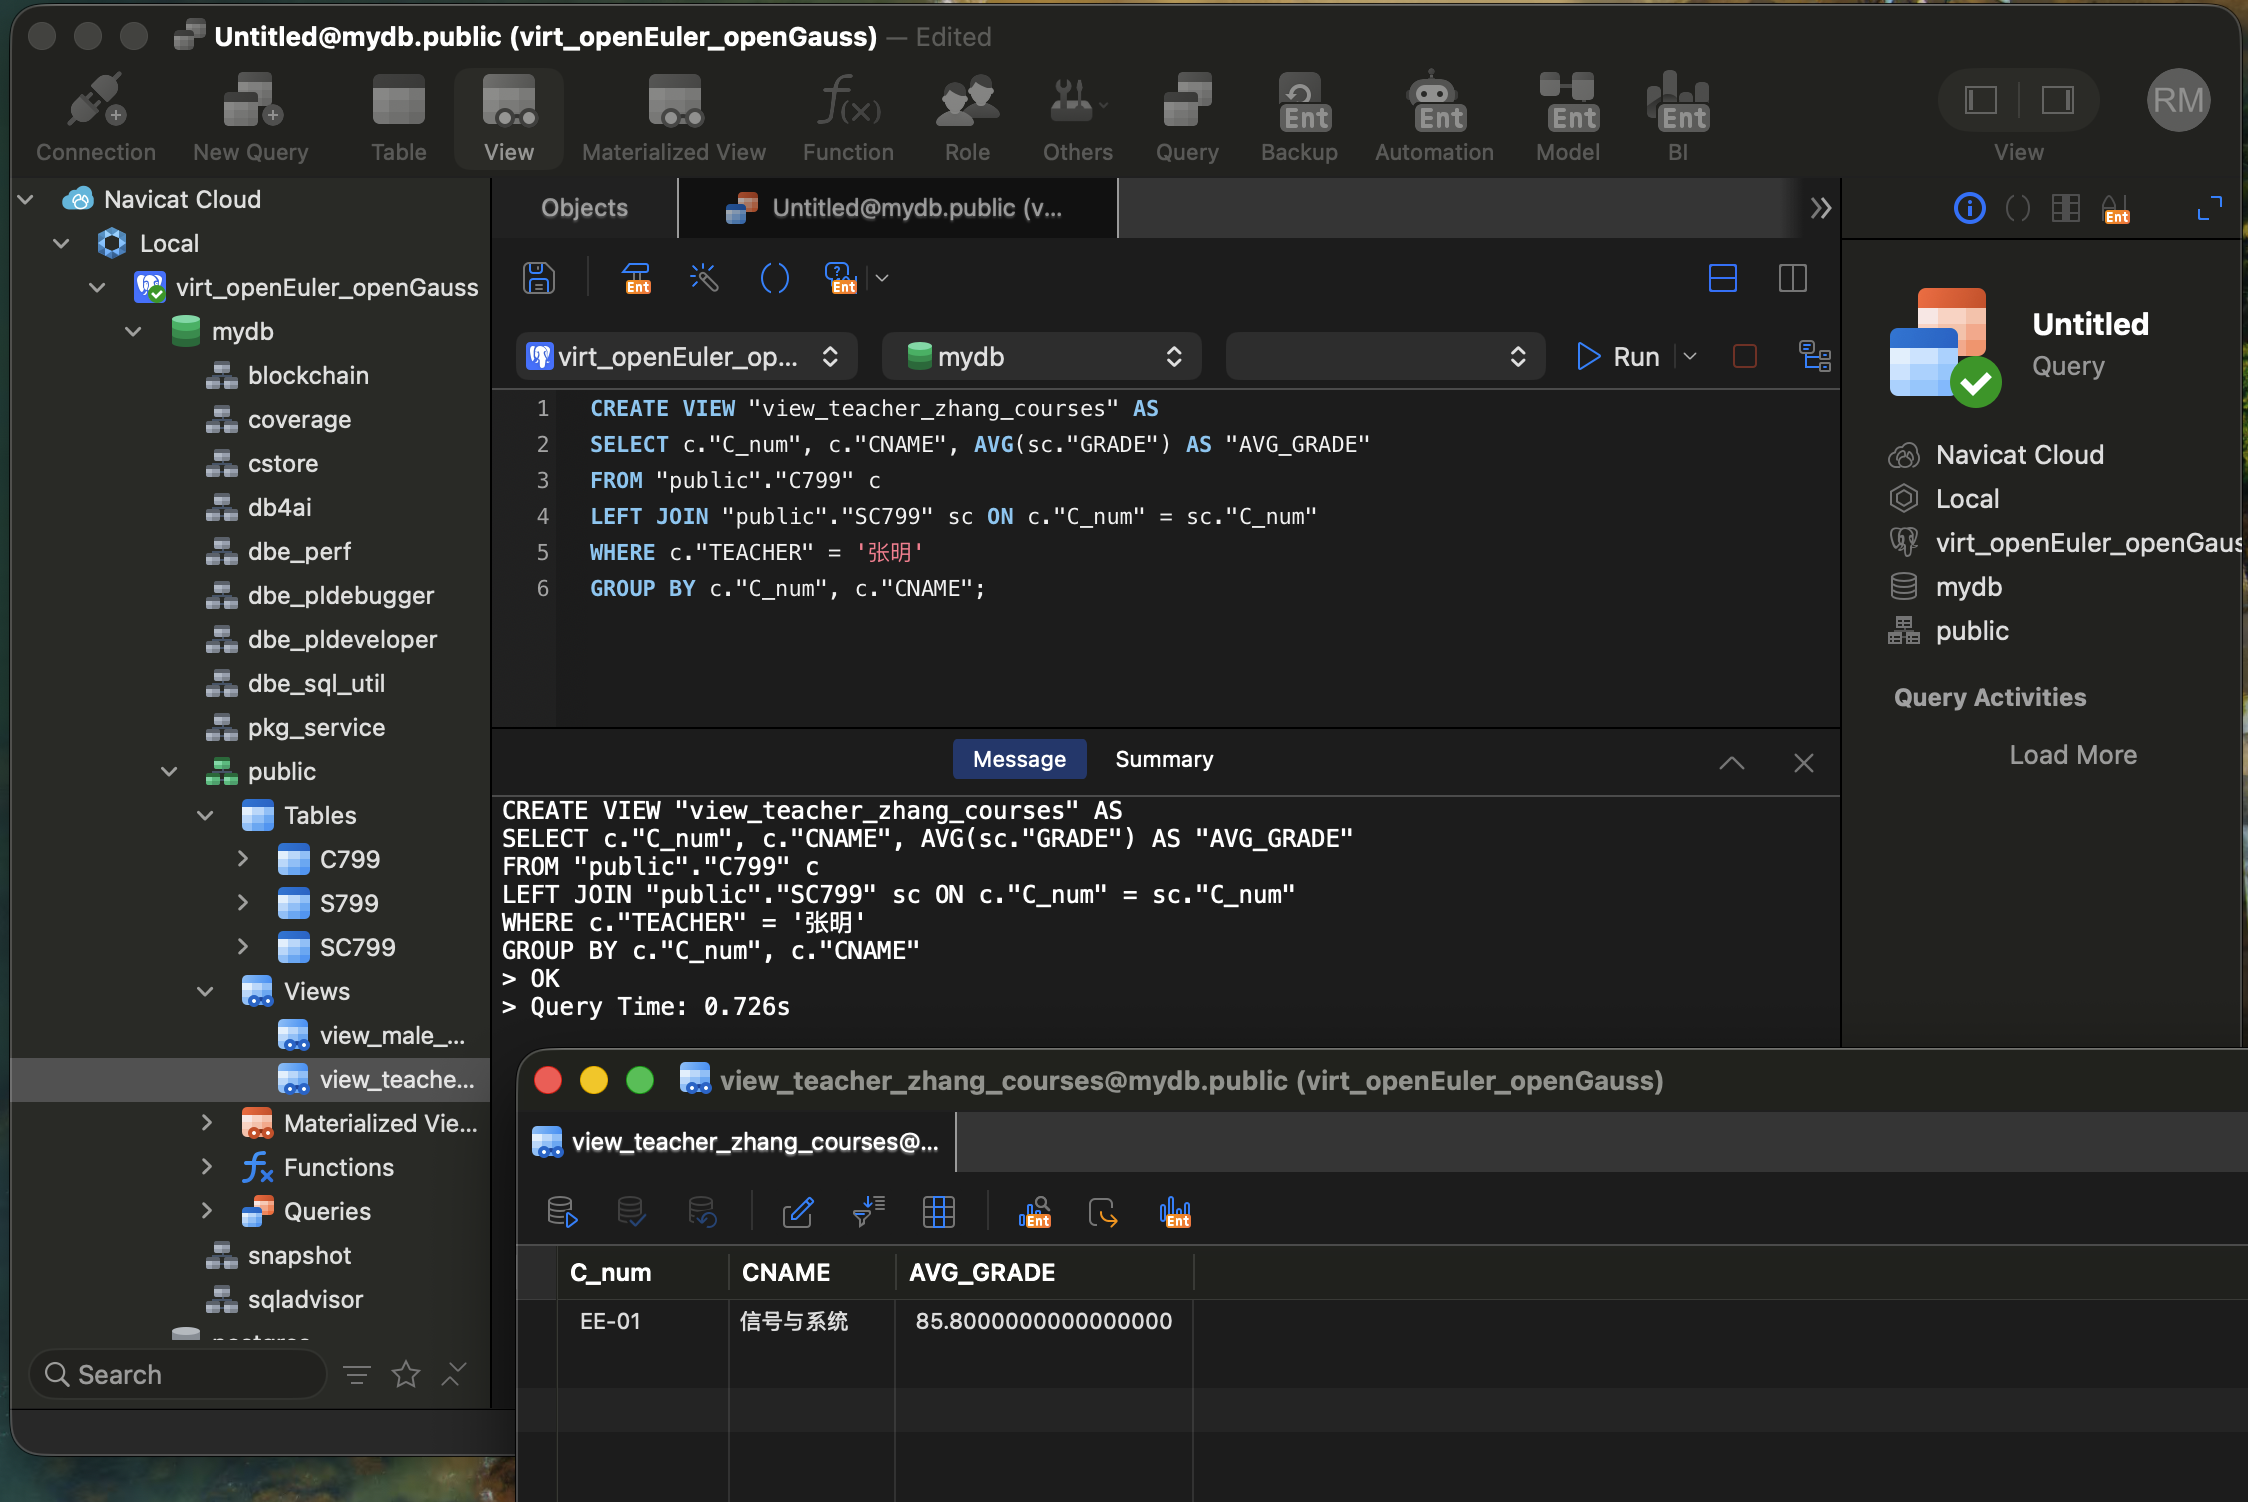
\includegraphics[width=0.88\textwidth]{images/20_3_5(2).png}
\caption{创建视图 view\_teacher\_zhang\_courses：张明老师所开课程及其平均成绩}
\label{fig:view2}
\end{figure}

视图中包含张明老师负责的"信号与系统"（EE-01），并通过聚合函数 \texttt{AVG} 计算选课学生的平均成绩。该视图将连接查询与聚合逻辑封装，使得后续查询只需 \texttt{SELECT * FROM view\_teacher\_zhang\_courses} 即可获取结果。

\paragraph{(3) 选修了"人工智能"课程的学生视图}

\begin{lstlisting}[style=sqlstyle]
CREATE VIEW "view_ai_students" AS
SELECT s."S_num", s."SNAME", sc."GRADE"
FROM "public"."S799" s
JOIN "public"."SC799" sc ON s."S_num" = sc."S_num"
JOIN "public"."C799"  c  ON sc."C_num" = c."C_num"
WHERE c."CNAME" = '人工智能';
\end{lstlisting}

\begin{figure}[H]
\centering
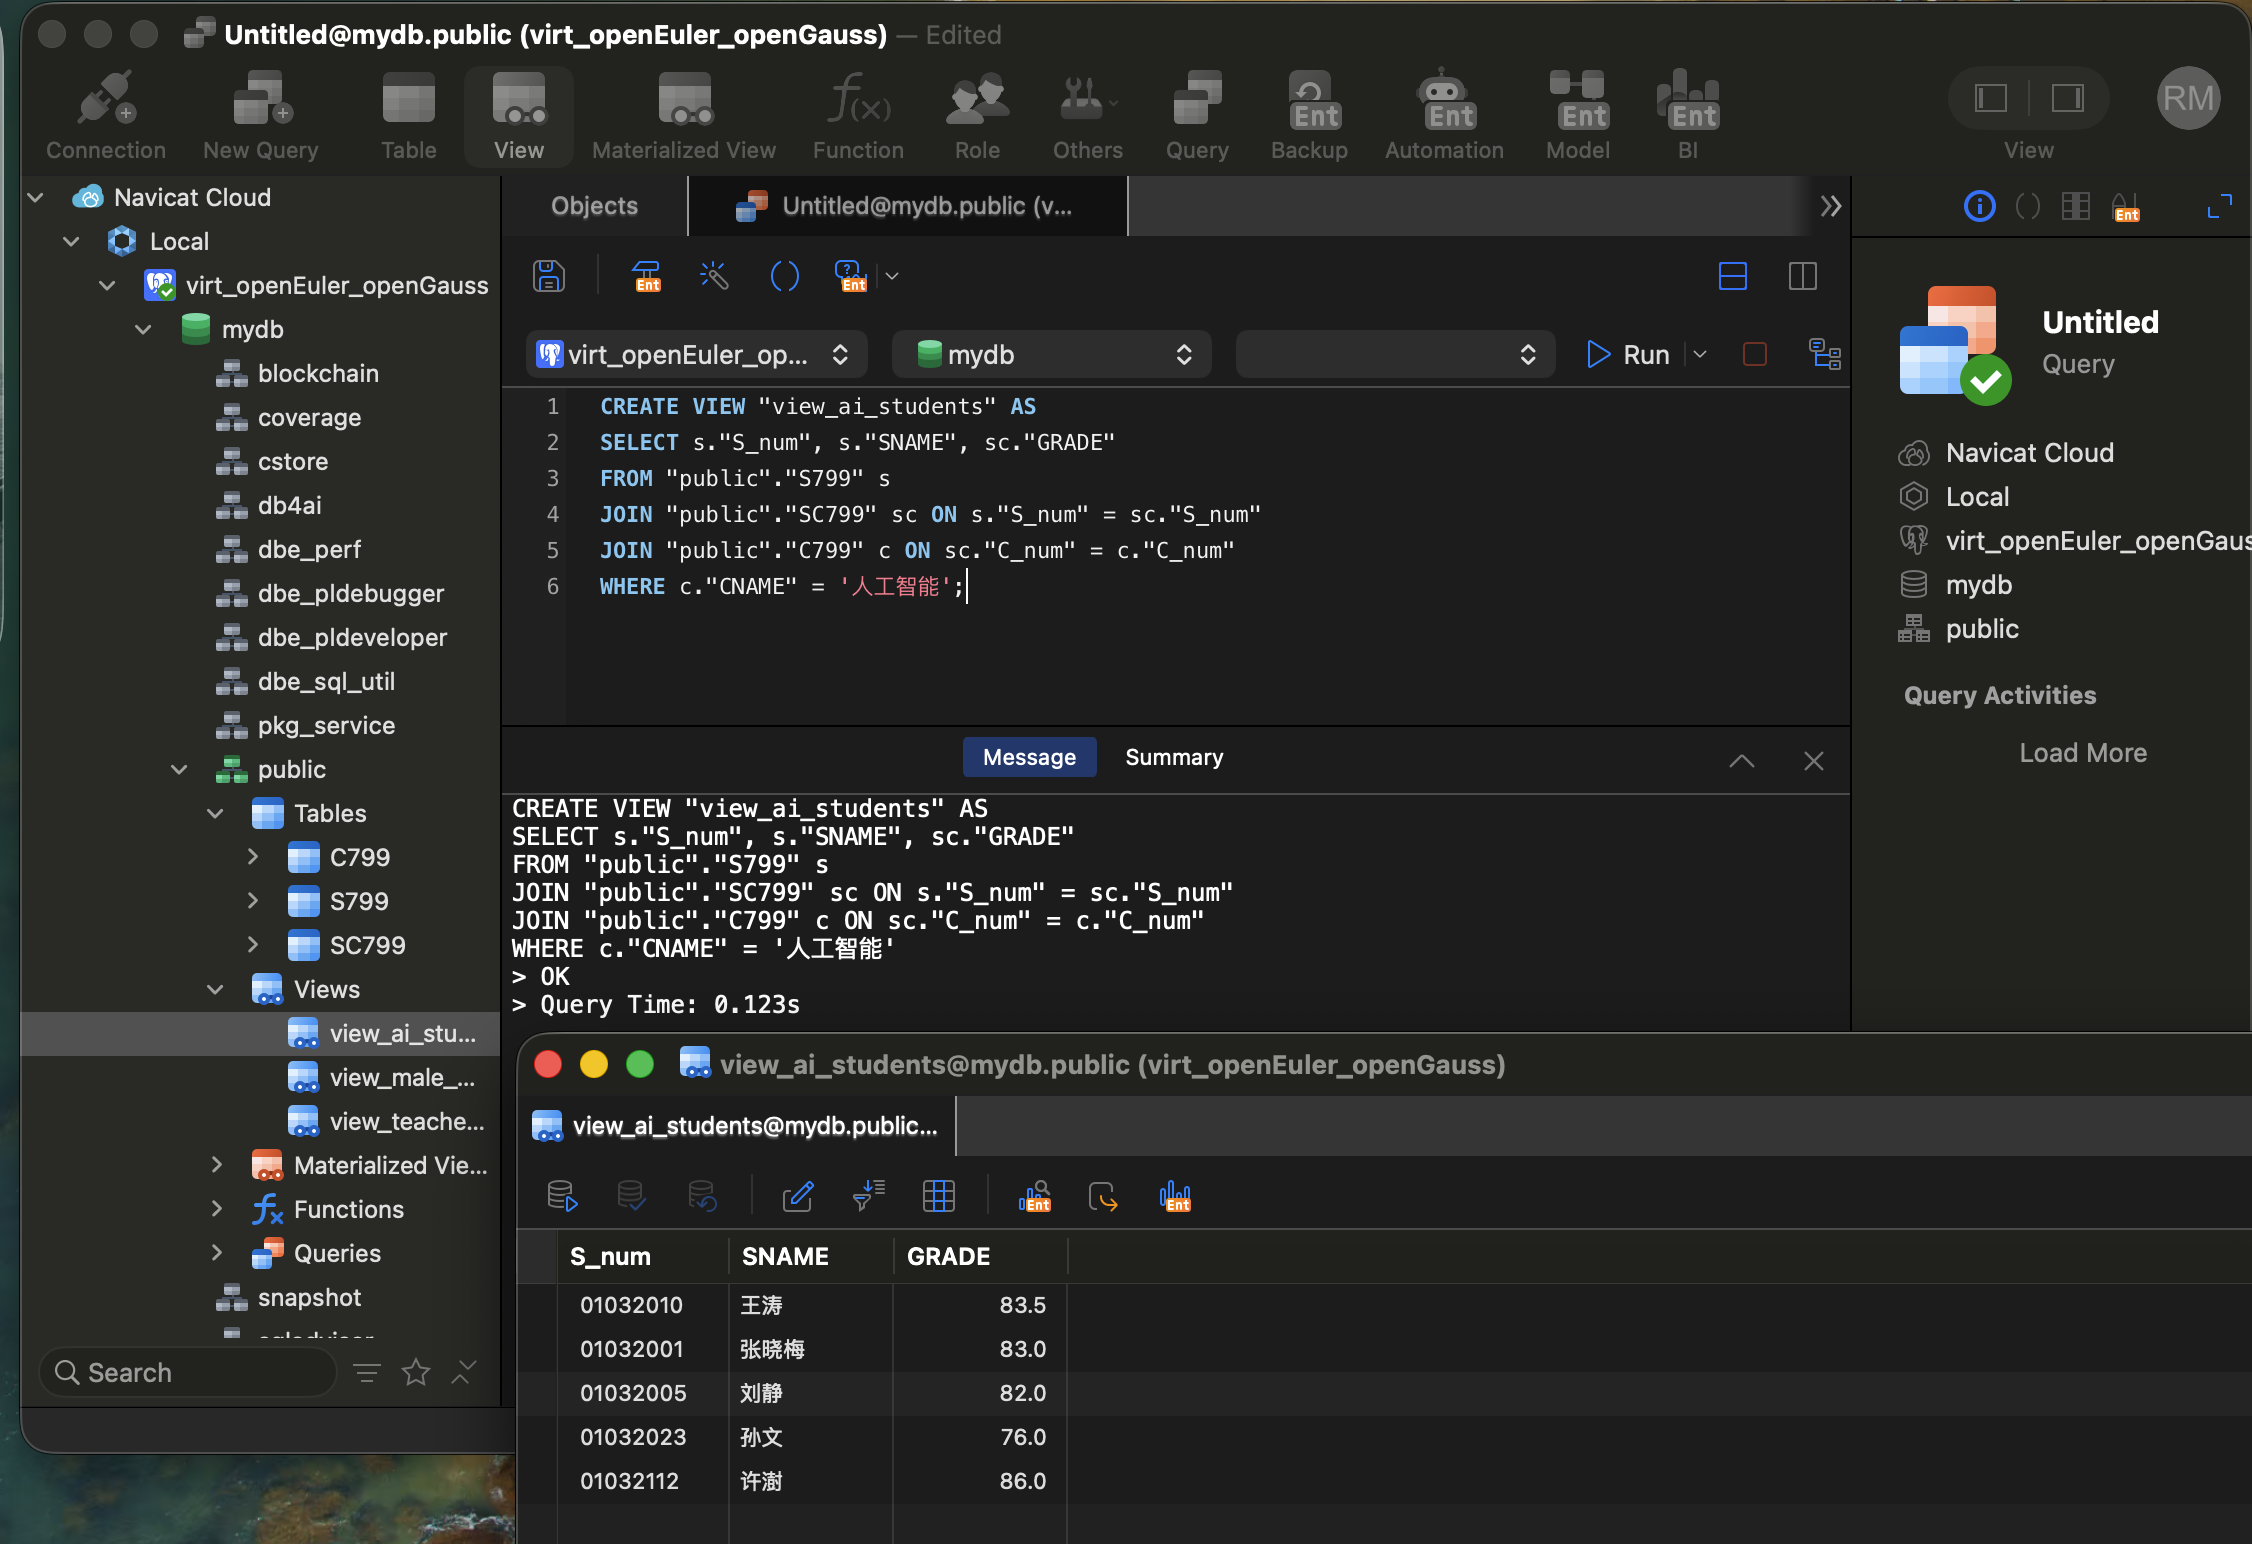
\includegraphics[width=0.88\textwidth]{images/21_3_5(3).png}
\caption{创建视图 view\_ai\_students：所有选修人工智能（CS-04）课程的学生}
\label{fig:view3}
\end{figure}

视图中包含 5 名选修人工智能（CS-04）的学生：王涛（83.5）、张晓梅（83.0）、刘静（82.0）、孙文（76.0）、许澍（86.0）。通过三表 JOIN 精确定位到课程名，比直接使用课程编号过滤更具可读性和鲁棒性。

\subsection{四、大规模数据生成与查询优化}

\subsubsection{四-1：多线程数据生成（目标：S799 约1000行，C799 约100行，SC799 约20000行）}

\paragraph{JDBC 连接测试}

在进行大规模数据写入前，首先通过 \texttt{ConnectionTestLocal.java} 验证 JDBC 驱动与数据库连接是否正常。程序加载 openGauss JDBC 驱动（\texttt{org.opengauss.Driver}），连接成功后执行一条简单的系统信息查询：

\begin{lstlisting}[style=javastyle]
Class.forName("org.opengauss.Driver");
String sql = "SELECT current_database(), current_user, version()";
try (Connection conn = DriverManager.getConnection(url, user, password);
     PreparedStatement stmt = conn.prepareStatement(sql);
     ResultSet rs = stmt.executeQuery()) {
    if (rs.next()) {
        System.out.println("Connection successful.");
        System.out.println("Database: "       + rs.getString(1));
        System.out.println("User: "           + rs.getString(2));
        System.out.println("Server version: " + rs.getString(3));
    }
}
\end{lstlisting}

\begin{figure}[H]
\centering
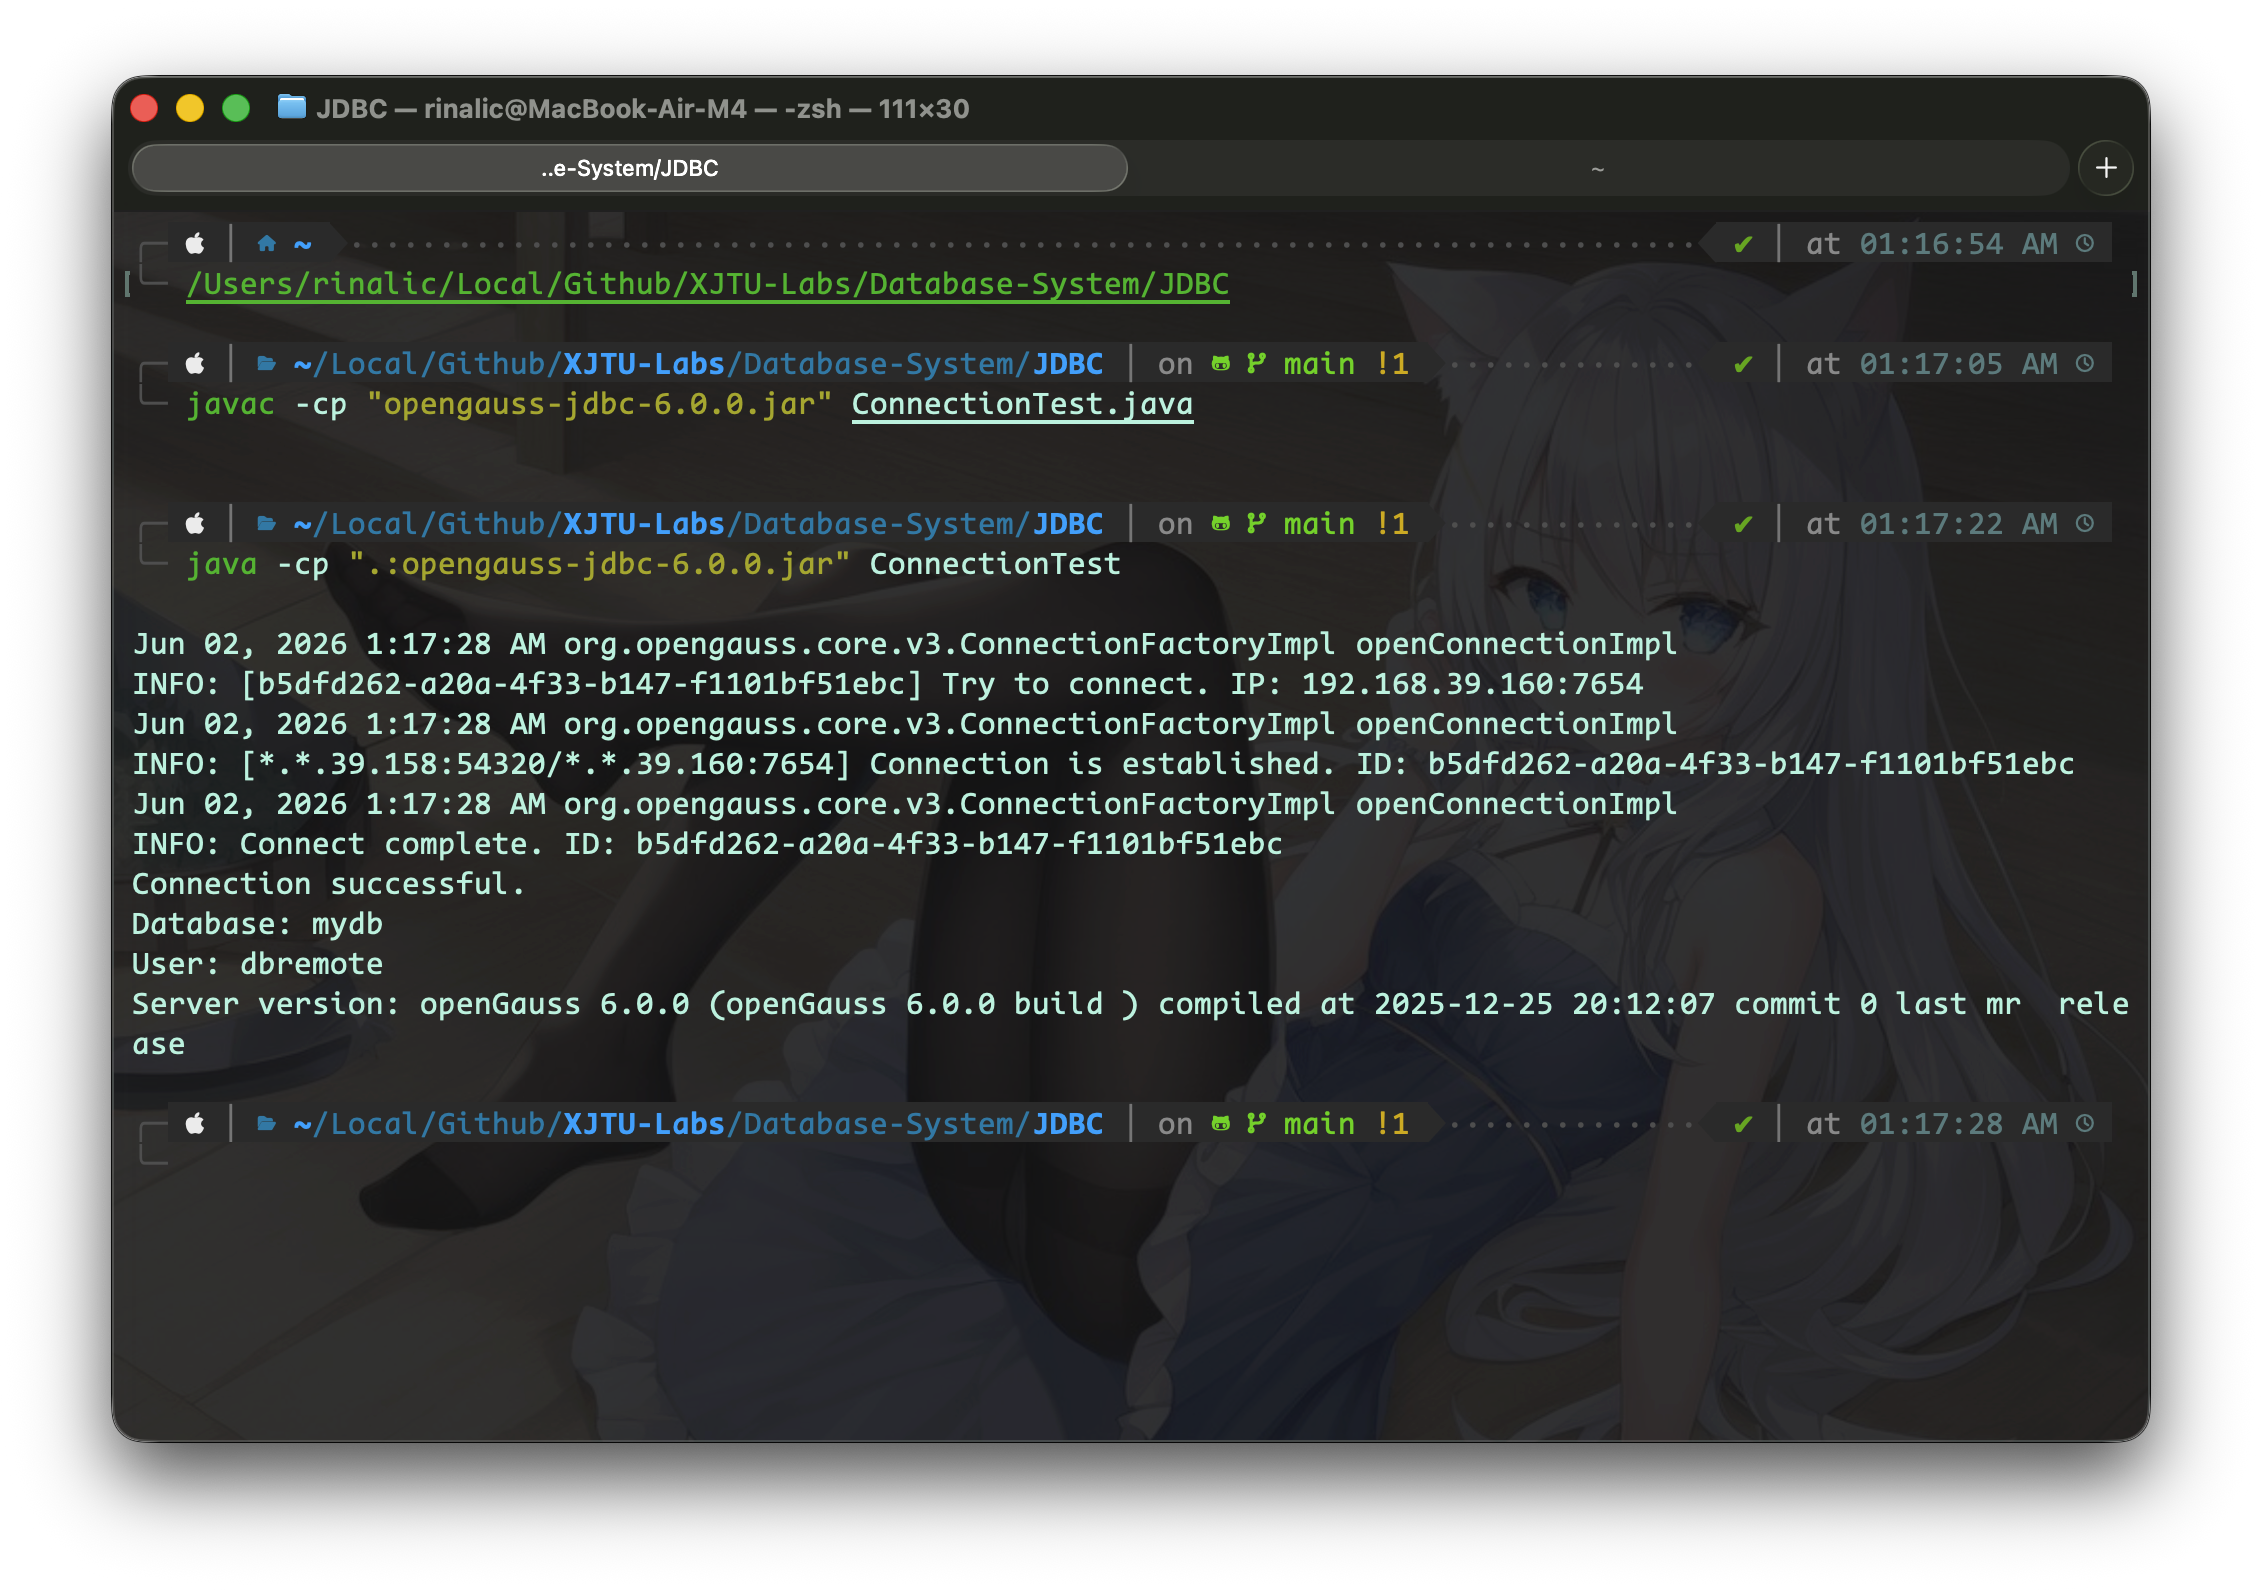
\includegraphics[width=0.88\textwidth]{images/22_4_0.png}
\caption{通过 JDBC 成功连接 openGauss 数据库的测试输出，显示数据库名、用户及服务器版本}
\label{fig:jdbc_connect}
\end{figure}

连接测试成功，程序正确输出了当前数据库名（mydb）、用户名（dbremote）以及 openGauss 服务器版本信息，确认 JDBC 驱动配置无误，可以进行后续的数据写入操作。

\paragraph{Python 脚本生成真实感数据}

为使生成数据更具真实性，实现了 Python 脚本 \texttt{generate\_names.py}，调用 RandomUser API（\url{https://randomuser.me/api/}）批量获取真实的英文姓名，同时生成可直接执行的 SQL 插入语句：

\begin{lstlisting}[style=pythonstyle]
API = "https://randomuser.me/api/"

def fetch_names(count):
    names = []
    left = count
    while left > 0:
        n = min(500, left)   # API 单次最多 500 条
        r = requests.get(API, params={"results": n, "nat": "us,gb,cn"})
        r.raise_for_status()
        for it in r.json().get("results", []):
            name = it["name"]
            names.append("{} {}".format(name["first"], name["last"]))
        left -= n
    return names
\end{lstlisting}

脚本执行后输出 \texttt{student\_names.txt}、\texttt{teacher\_names.txt} 等姓名列表文件，供 Java 数据生成器按索引循环使用。脚本同时生成 SQL 文件（\texttt{students.sql}、\texttt{courses.sql}、\texttt{enrollments.sql}），可直接通过 \texttt{psql} 导入。

\begin{verbatim}
python generate_names.py --students 1000 --courses 100 \
    --enrollments 20000 --outdir ./sql_out
\end{verbatim}

\begin{figure}[H]
\centering
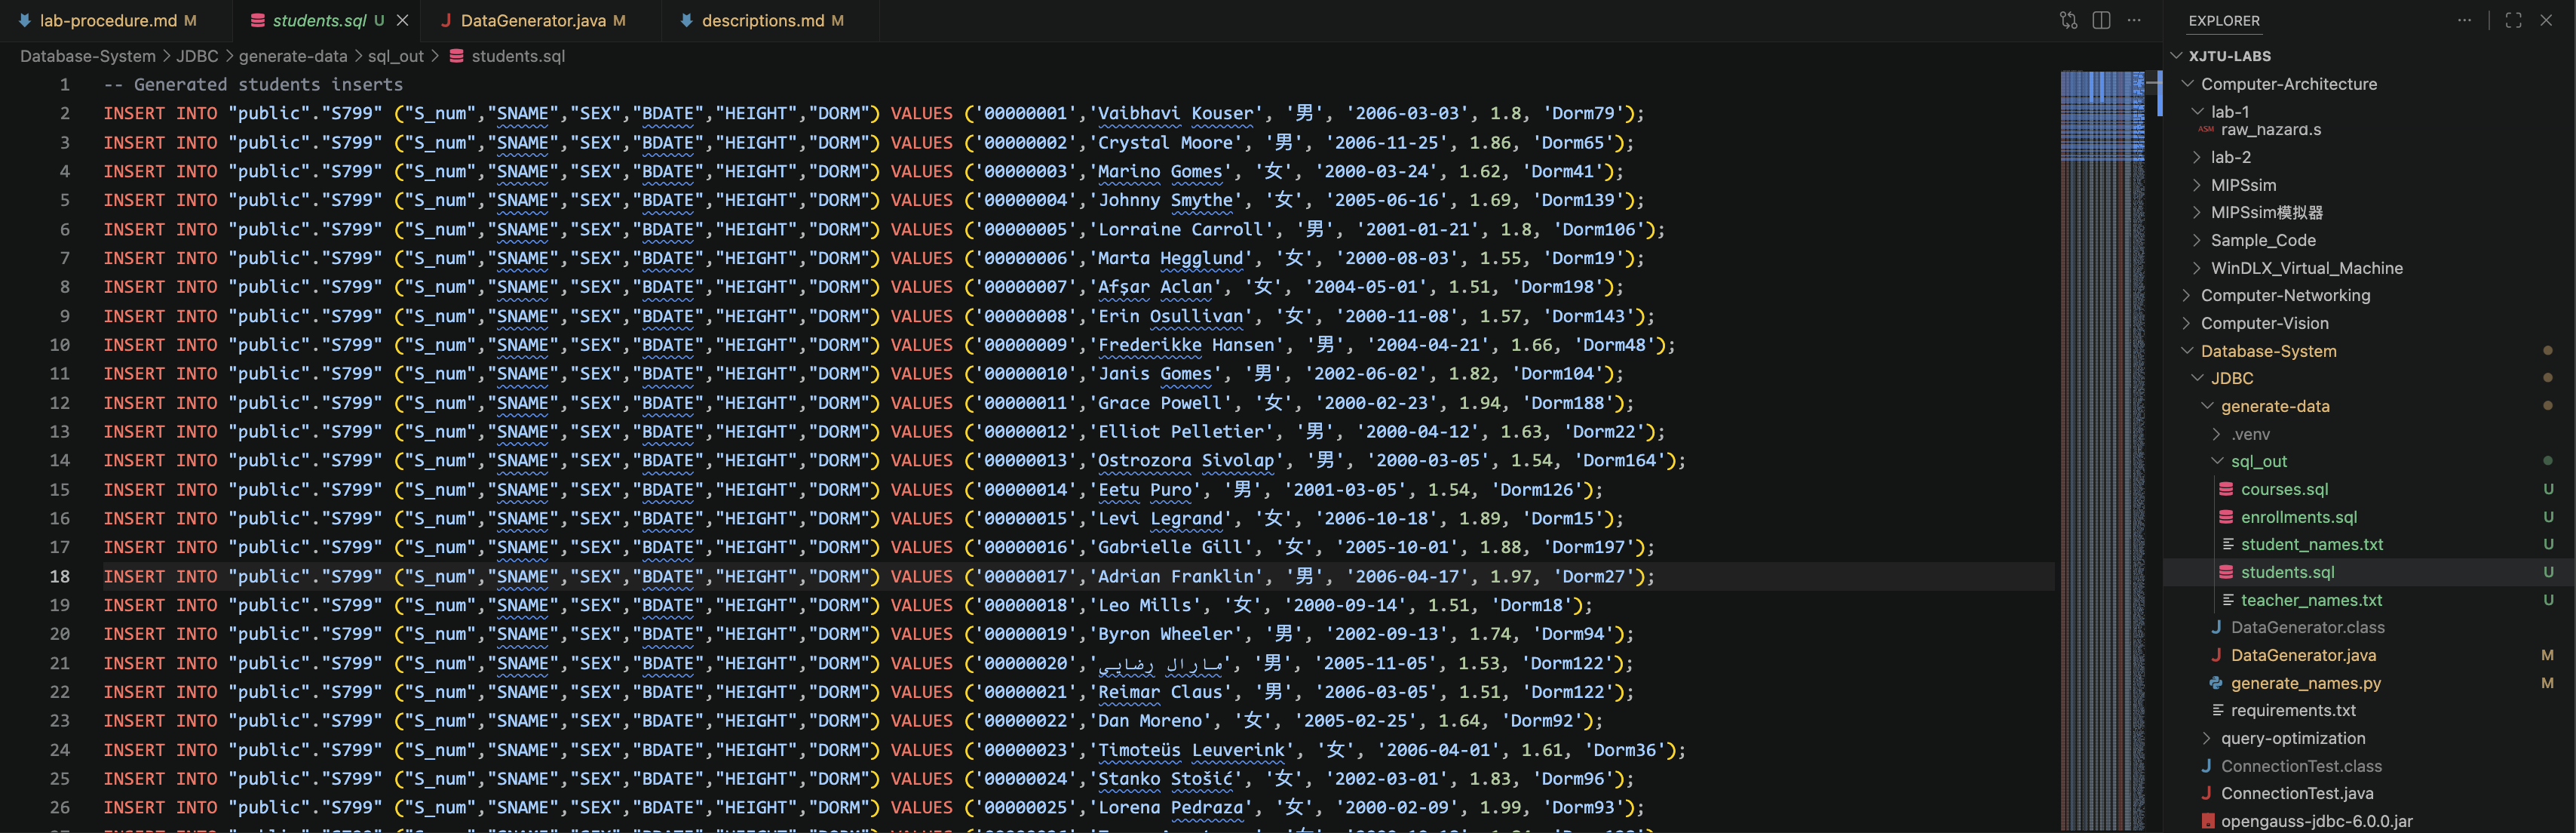
\includegraphics[width=0.88\textwidth]{images/23_4_1_1.png}
\caption{Python 脚本从 RandomUser API 获取的学生姓名数据示例（部分）}
\label{fig:py_gen}
\end{figure}

\paragraph{Java 多线程批量写入}

\texttt{DataGenerator.java} 实现了多线程批量写入，核心设计要点如下：

\begin{enumerate}
  \item \textbf{多线程分区}：使用 \texttt{ExecutorService} 固定线程池（默认 8 线程），将待插入数据按批次（学生每批 200 条，选课每批 1000 条）分配给各线程并行处理，每个线程独立持有一个 \texttt{Connection}，避免连接竞争与锁等待。

  \item \textbf{批量提交（Batch Insert）}：使用 \texttt{PreparedStatement.addBatch()} 积累多条插入后一次性调用 \texttt{executeBatch()}，将多条 INSERT 合并为单次网络往返，显著降低通信开销。

  \item \textbf{事务控制}：每批次关闭自动提交（\texttt{setAutoCommit(false)}），执行 batch 后调用 \texttt{commit()}，保证批次的原子性——要么全部成功，要么全部回滚。

  \item \textbf{随机 NULL 成绩注入}：在生成选课记录时，以 8\% 的概率将 \texttt{GRADE} 设置为 NULL（\texttt{ps.setNull(3, Types.DECIMAL)}），模拟真实的"已选课但未有成绩"情形。

  \item \textbf{低分记录删除}：数据生成完成后，利用 \texttt{ctid} 子查询精确定位并删除 200 条成绩低于 60 分或为 NULL 的记录，\texttt{ctid} 是 openGauss 内部行标识符，可精确控制删除行数：
\end{enumerate}

\begin{lstlisting}[style=javastyle]
// 多线程学生数据写入（核心结构）
ExecutorService es = Executors.newFixedThreadPool(threads);
for (int start = 1; start <= n; start += batch) {
    final int s = start, end = Math.min(n, start + batch - 1);
    es.submit(() -> {
        try (Connection conn = DriverManager.getConnection(URL,USER,PASS)) {
            conn.setAutoCommit(false);
            PreparedStatement ps = conn.prepareStatement(insertSQL);
            for (int i = s; i <= end; i++) {
                ps.setString(1, id);   // S_num
                ps.setString(2, name); // SNAME
                // ... 设置其余字段 ...
                ps.addBatch();
            }
            ps.executeBatch();
            conn.commit();
        }
    });
}
es.shutdown();
es.awaitTermination(1, TimeUnit.HOURS);
\end{lstlisting}

\begin{lstlisting}[style=javastyle]
// 使用 ctid 删除固定数量的低分/NULL 记录
String sql =
    "DELETE FROM \"public\".\"SC799\" WHERE ctid IN (" +
    "  SELECT ctid FROM \"public\".\"SC799\" " +
    "  WHERE (\"GRADE\" < 60 OR \"GRADE\" IS NULL) LIMIT ?)";
PreparedStatement ps = conn.prepareStatement(sql);
ps.setInt(1, 200);
int deleted = ps.executeUpdate();
System.out.println("Deleted " + deleted + " low-grade records.");
\end{lstlisting}

\begin{figure}[H]
\centering
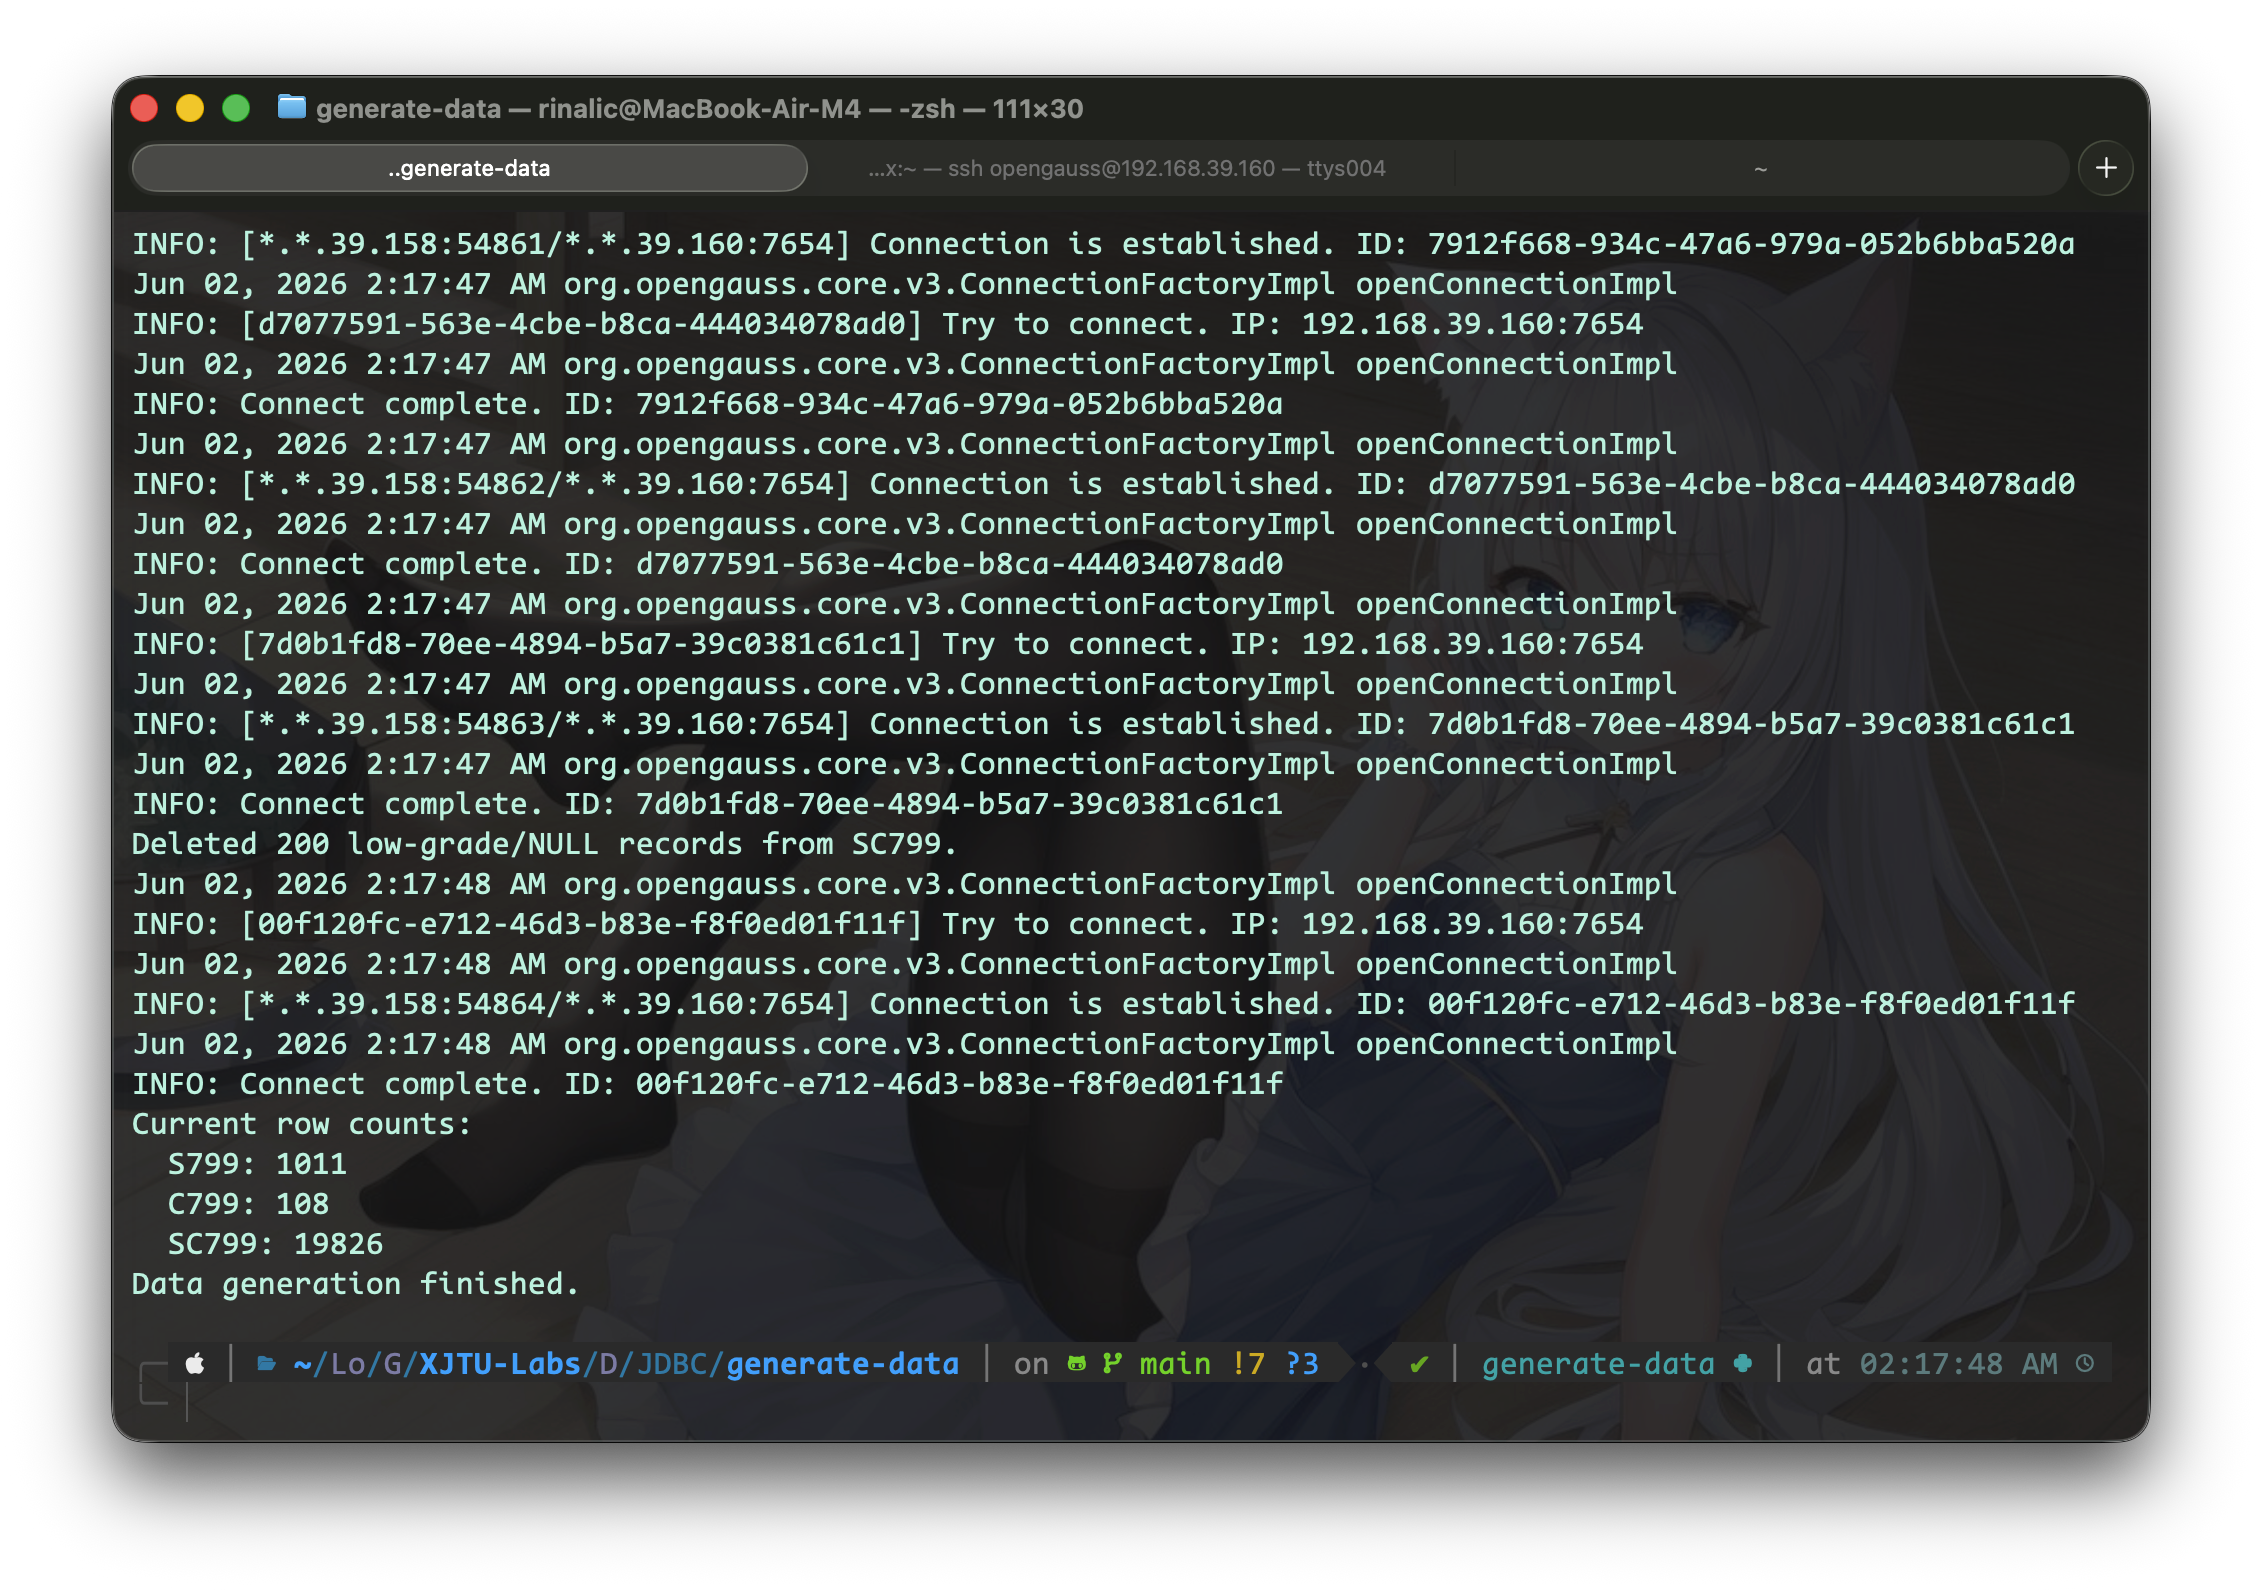
\includegraphics[width=0.88\textwidth]{images/24_4_1_2.png}
\caption{Java 多线程数据生成程序的终端输出，展示各表写入数量与删除记录数}
\label{fig:java_output}
\end{figure}

\begin{figure}[H]
\centering
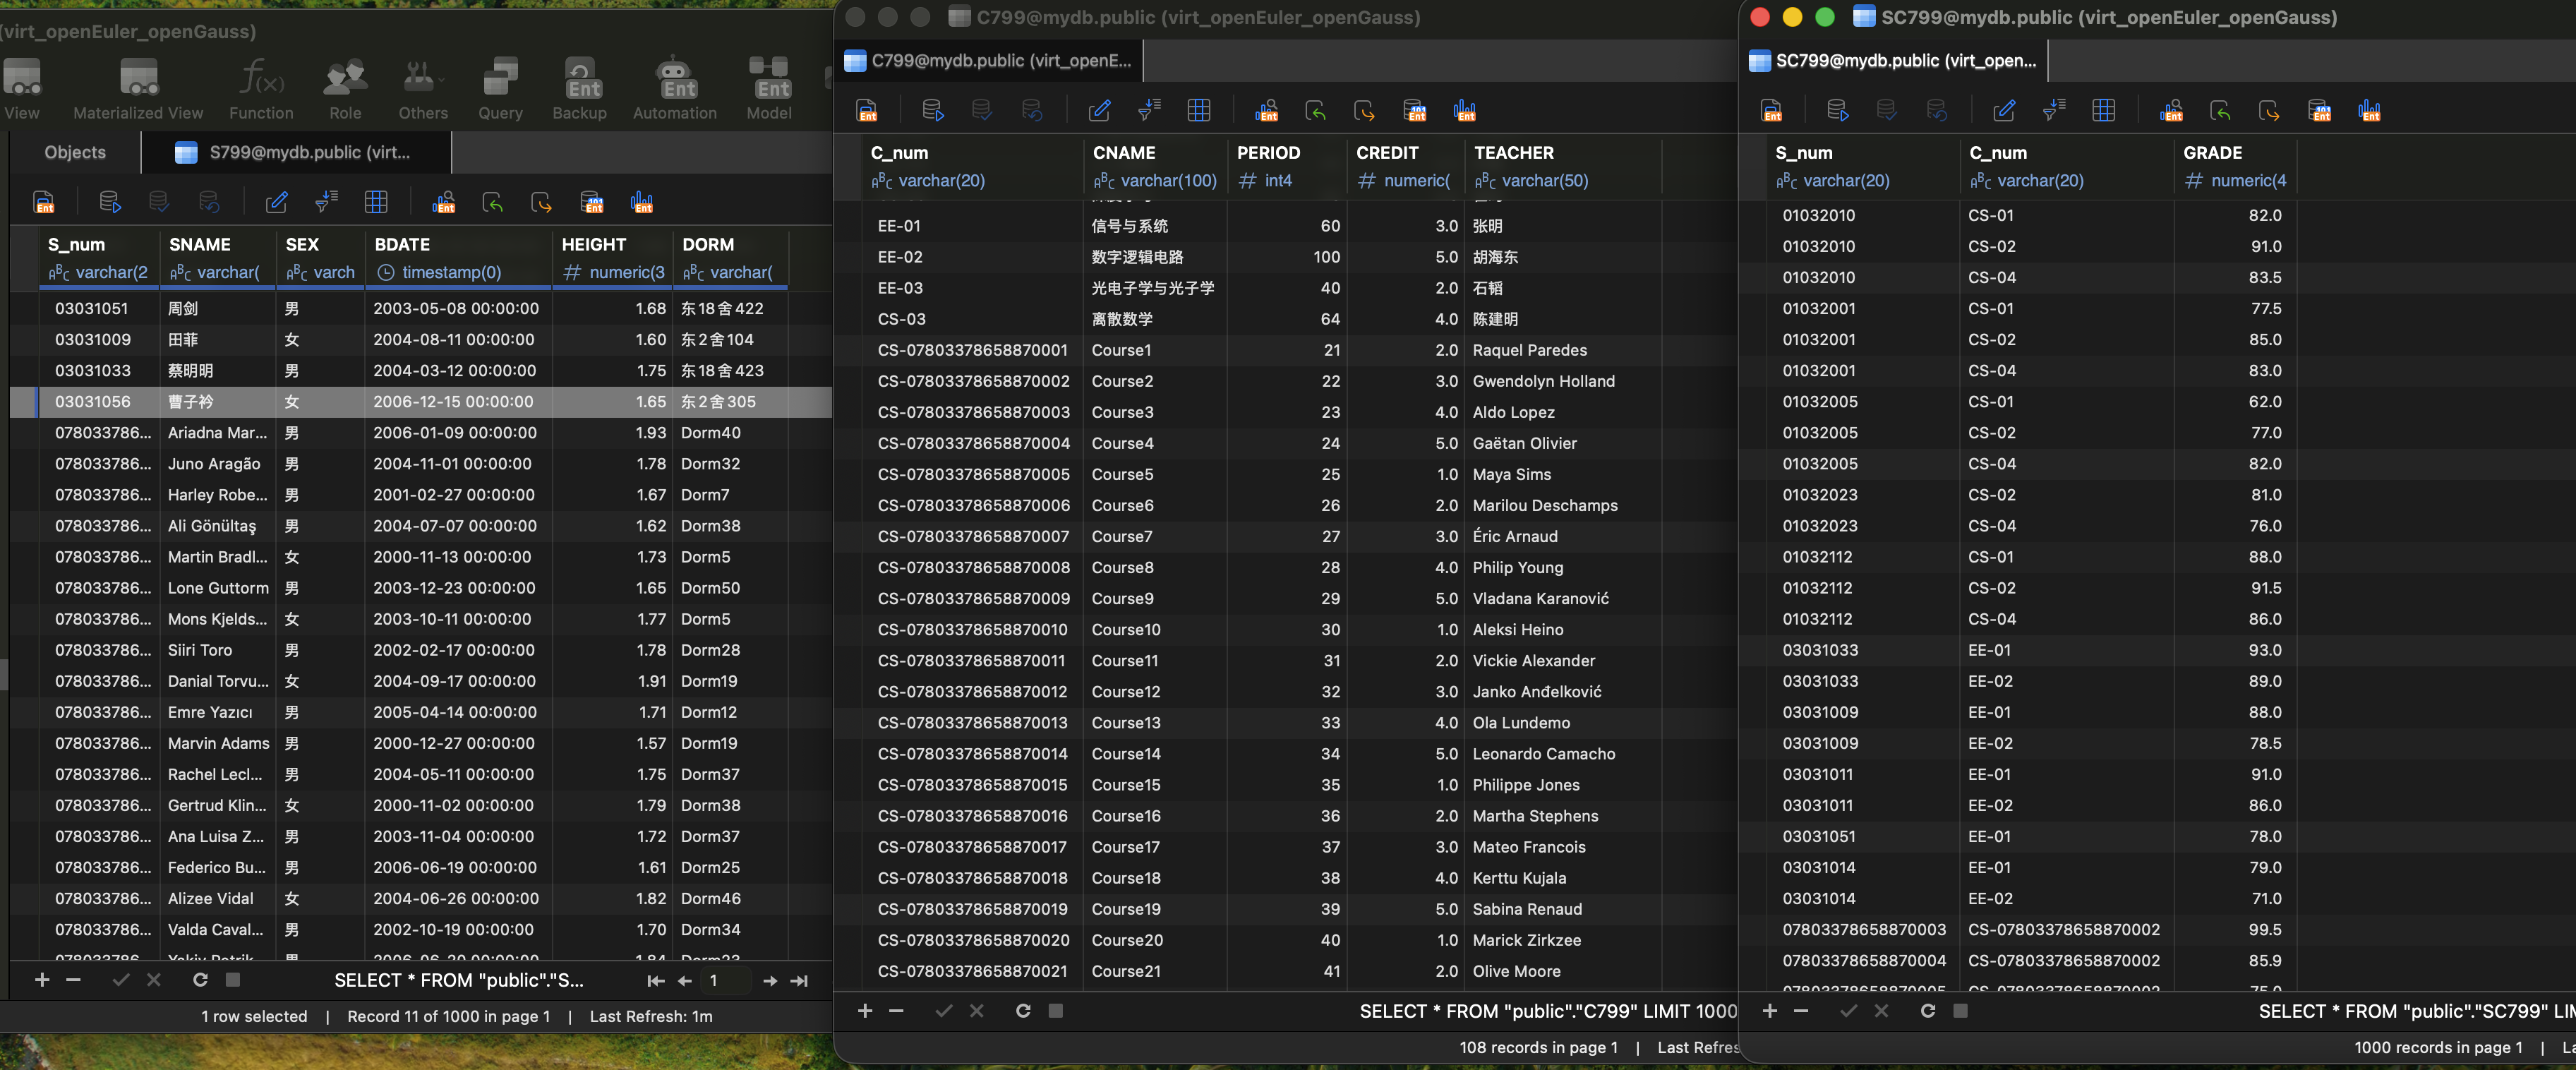
\includegraphics[width=0.88\textwidth]{images/25_4_1_3.png}
\caption{数据写入完成后，在 Navicat 中查看 S799、C799、SC799 三张表的实际数据量}
\label{fig:navicat_count}
\end{figure}

数据写入完成后，S799 约有 1000 行，C799 约有 100 行，SC799 约有 19800 行（20000 条生成后扣除 200 条低分删除），满足实验第四-1 题的规模要求。多线程并发写入相比单线程串行写入显著缩短了执行时间。

\subsubsection{四-2：大规模数据与查询优化（目标：S799 约5000行，C799 约1000行，SC799 约200000行）}

\paragraph{数据规模扩展}

使用 \texttt{DataGenerator.java} 的 \texttt{--task2} 参数一键扩展至目标规模（S799 约 5000 行，C799 约 1000 行，SC799 约 200000 行）：

\begin{verbatim}
java -cp ".:../opengauss-jdbc-6.0.0.jar" DataGenerator --task2
\end{verbatim}

\begin{figure}[H]
\centering
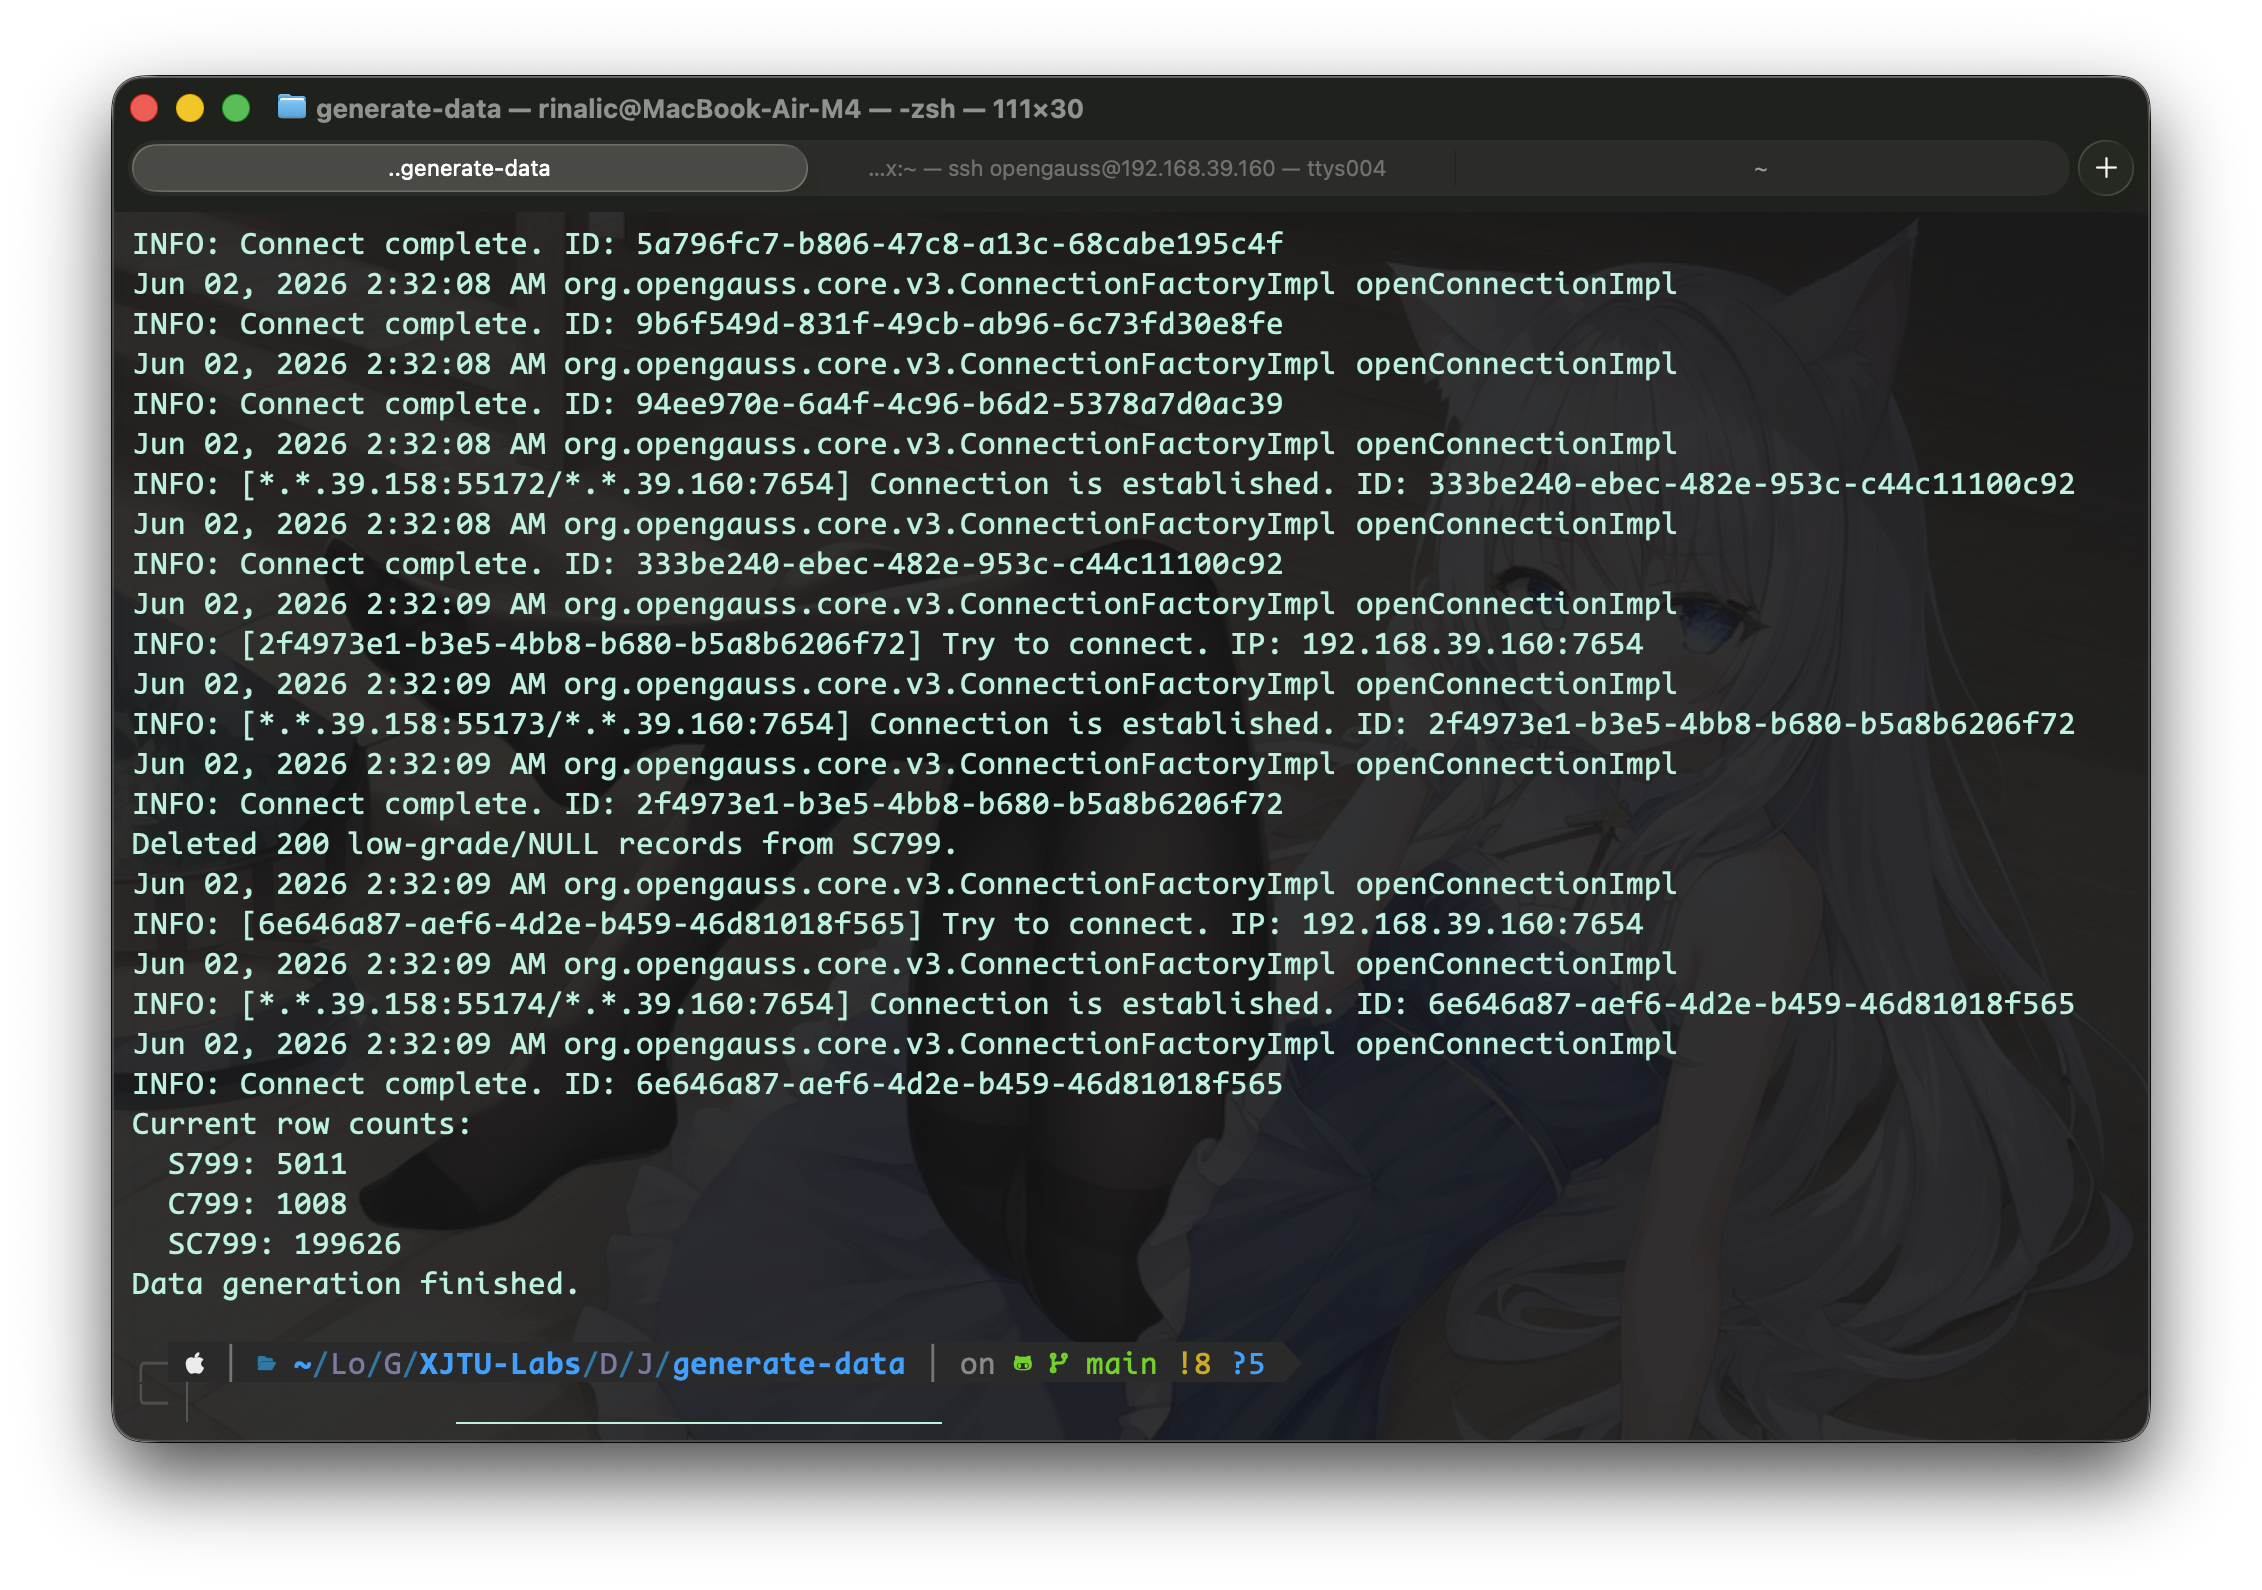
\includegraphics[width=0.88\textwidth]{images/26_4_2_1.png}
\caption{第二轮数据扩展的终端输出，三张表数据量分别达到约 5000/1000/200000 行}
\label{fig:task2_output}
\end{figure}

\paragraph{索引策略}

在 SC799 表上为常用查询路径创建 B-Tree 索引，覆盖课程编号过滤、学号过滤、联合查询和成绩非空过滤四种场景：

\begin{lstlisting}[style=sqlstyle]
-- 课程编号索引（加速 WHERE "C_num" = ? 过滤）
CREATE INDEX IF NOT EXISTS idx_sc799_cnum
  ON "public"."SC799" ("C_num");

-- 学号索引（加速 WHERE "S_num" = ? 过滤）
CREATE INDEX IF NOT EXISTS idx_sc799_snum
  ON "public"."SC799" ("S_num");

-- 联合索引（支持按课程+学号联合查询的覆盖扫描）
CREATE INDEX IF NOT EXISTS idx_sc799_cnum_snum
  ON "public"."SC799" ("C_num", "S_num");

-- 部分索引（仅对非 NULL 成绩建立，减小索引体积）
CREATE INDEX IF NOT EXISTS idx_sc799_grade_notnull
  ON "public"."SC799" ("GRADE")
  WHERE "GRADE" IS NOT NULL;
\end{lstlisting}

\paragraph{查询变体与执行计划对比}

使用 Python 自动化实验驱动器 \texttt{optimization\_driver.py} 对以下 5 种查询变体分 3 次重复运行，通过 \texttt{EXPLAIN (ANALYZE, BUFFERS)} 收集实际执行时间与执行计划：

\begin{itemize}
  \item \textbf{Query 1}：三-1.(4) 标准实现——LEFT JOIN 三表后 GROUP BY 求总学分
  \item \textbf{Query 2}：三-1.(4) 预筛选变体——先过滤非 NULL 成绩子查询，再 JOIN 计算学分
  \item \textbf{Query 3}：三-1.(6) 标准实现——HAVING + 子查询对比均值
  \item \textbf{Query 4}：三-1.(8) 标准实现——HAVING COUNT >= 3 后 ORDER BY AVG DESC LIMIT 1
  \item \textbf{Query 5}：三-1.(8) CTE 变体——使用 WITH 子句将聚合与排序分离
\end{itemize}

运行驱动器的命令如下：

\begin{verbatim}
python optimization_driver.py \
    --host 192.168.39.160 --port 7654 --dbname mydb \
    --user dbremote --password 'dbremote:399' \
    --apply-indexes --run-queries --repeats 3 --analyze-after-ddl
\end{verbatim}

\paragraph{实验结果}

实验结果汇总如下表：

\begin{table}[H]
\centering
\caption{各查询变体在 SC799 约 200000 行规模下的平均执行时间}
\label{tab:opt}
\begin{tabular}{clrr}
\toprule
查询编号 & 对应题目与描述 & 平均总耗时 (ms) & 平均计划执行时间 (ms) \\
\midrule
Query 1 & 三-1(4) 标准 LEFT JOIN & 172.4 & 149.8 \\
Query 2 & 三-1(4) 预筛选子查询变体 & 174.0 & 140.6 \\
Query 3 & 三-1(6) HAVING 子查询 & 174.0 & 155.5 \\
Query 4 & 三-1(8) 直接 HAVING+ORDER BY & 173.8 & 142.3 \\
Query 5 & 三-1(8) CTE 分离聚合版 & 174.3 & 146.1 \\
\bottomrule
\end{tabular}
\end{table}

以 Query 1 的实际执行计划为例：

\begin{verbatim}
HashAggregate  (cost=11126.60..11176.71 rows=5011 width=69)
               (actual time=149.270..149.796 rows=5011 loops=1)
  Group By Key: s."S_num", s."SNAME"
  ->  Hash Left Join  (actual time=1.279..88.742 rows=199627)
        Hash Cond: sc."C_num" = c."C_num"
        ->  Hash Right Join  (actual time=1.063..52.913 rows=199627)
              ->  Seq Scan on "SC799" sc  (actual time=0.003..11.316
                                           rows=199626)
              ->  Seq Scan on "S799"  s   (actual time=0.005..0.461
                                           rows=5011)
        ->  Seq Scan on "C799"  c         (actual time=0.002..0.090
                                           rows=1008)
Total runtime: 150.099 ms
\end{verbatim}

\paragraph{深入分析}

\begin{itemize}
  \item \textbf{优化器选择全表顺序扫描（Seq Scan）而非索引扫描}：五个查询变体执行时间非常接近（均在 140--175 ms 范围内）。根本原因在于，这三个查询（(4)(6)(8)）均为\textbf{聚合型查询}，需要扫描 SC799 几乎全部近 20 万行记录来计算 SUM/AVG/COUNT。对于这种\textbf{低选择性}的全表聚合，B-Tree 索引无法带来显著收益——读完整个索引反而比顺序读堆表更慢，优化器正确选择了 Seq Scan。

  \item \textbf{哈希连接（Hash Join）的高效性}：大表间全量 JOIN 时，Hash Join 比嵌套循环（Nested Loop）+索引查找更高效，因为它只需一次全扫描即可建立哈希表，无需对每行外表记录反复读取索引页。执行计划中三表连接均采用 Hash Left Join / Hash Right Join，体现了优化器的合理选择。

  \item \textbf{CTE 与直接写法等效}：Query 4（HAVING + ORDER BY）与 Query 5（CTE 版）执行时间几乎相同，说明 openGauss 优化器对简单 CTE 执行了内联展开（inline），消除了中间物化的额外代价。

  \item \textbf{索引对高选择性点查询效果显著}：虽然本次对比的聚合查询受益有限，但若将查询改为 \texttt{WHERE "C\_num" = 'CS-01'} 这样的精确过滤，\texttt{idx\_sc799\_cnum} 索引可使优化器切换为 Index Scan，将 I/O 从全表约 20 万行降至几百行，优化效果将非常显著。

  \item \textbf{优化建议}：对当前聚合场景，可考虑（1）建立物化视图（Materialized View）预计算聚合结果；（2）对 SC799 按 \texttt{S\_num} 进行范围分区，缩小每次聚合的扫描范围；（3）针对特定选择性谓词添加覆盖索引，配合 \texttt{/*+ IndexScan(sc799 idx\_sc799\_cnum) */} Hint 引导优化器走索引路径。
\end{itemize}

\subsection{五、数据库备份与恢复}

\subsubsection{数据库备份}

完成全部实验操作后，使用 openGauss 提供的逻辑备份工具 \texttt{gs\_dump} 对 mydb 数据库进行全量备份。实验过程中共保留了多个阶段性快照：

\begin{itemize}
  \item \texttt{0\_before-4.sql}：实验第四题开始前、仅含初始数据的备份
  \item \texttt{1\_before\_4.2.sql}：四-1 完成后、扩展至大规模前的备份
  \item \texttt{2\_before\_opt.sql}：建立索引并运行优化实验前的备份
  \item \texttt{3\_before\_null\_del.sql}：执行第六题触发器删除前的备份
\end{itemize}

备份命令格式如下：

\begin{verbatim}
gs_dump -U dbremote -W dbremote:399 \
        -h 192.168.39.160 -p 7654 \
        mydb -f mydb-backup.sql
\end{verbatim}

\subsubsection{恢复合作同学的备份}

从合作同学处接收其 mydb 数据库的逻辑备份文件 \texttt{partner.sql}，在本地 openGauss 实例中创建独立数据库后执行恢复：

\begin{verbatim}
# 创建用于恢复的独立数据库
gsql -U dbremote -W dbremote:399 -h 192.168.39.160 -p 7654 \
     -d postgres -c "CREATE DATABASE partner_db;"

# 将备份内容恢复至 partner_db
gsql -U dbremote -W dbremote:399 -h 192.168.39.160 -p 7654 \
     -d partner_db -f partner.sql
\end{verbatim}

\begin{figure}[H]
\centering
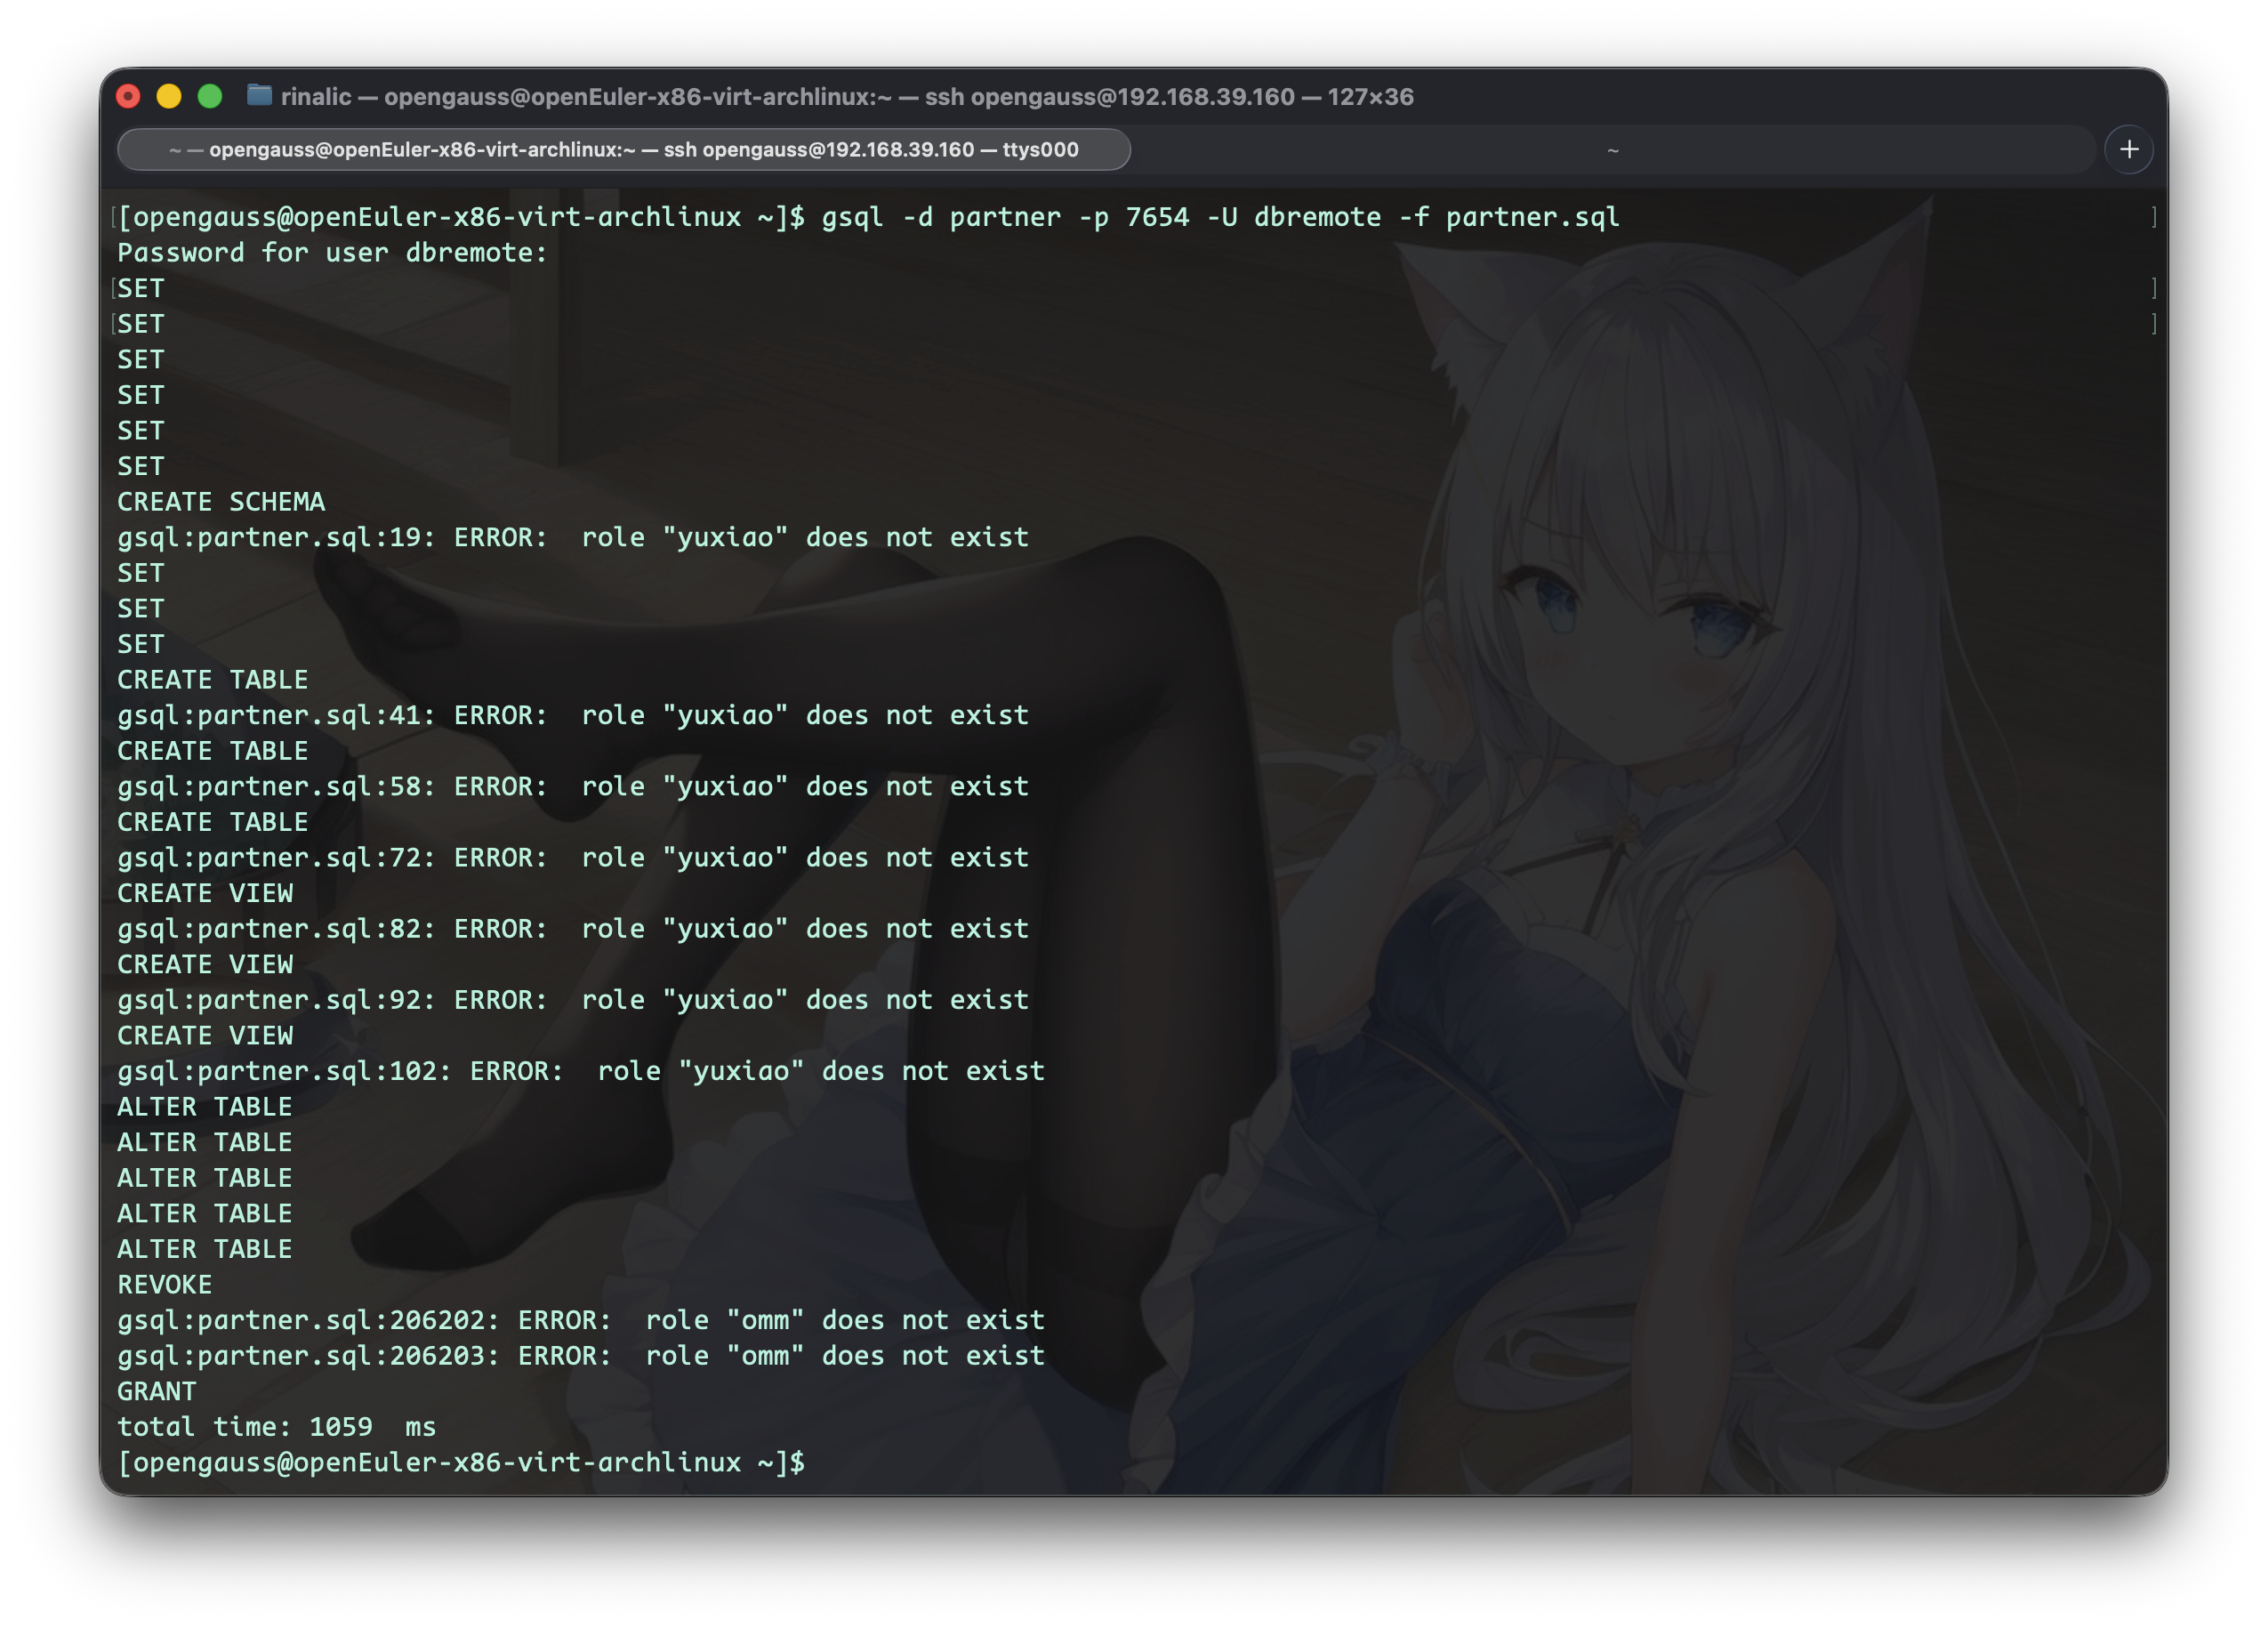
\includegraphics[width=0.88\textwidth]{images/27_5_1.png}
\caption{终端执行恢复命令，成功将合作同学的数据库备份还原至 partner\_db}
\label{fig:restore_terminal}
\end{figure}

\begin{figure}[H]
\centering
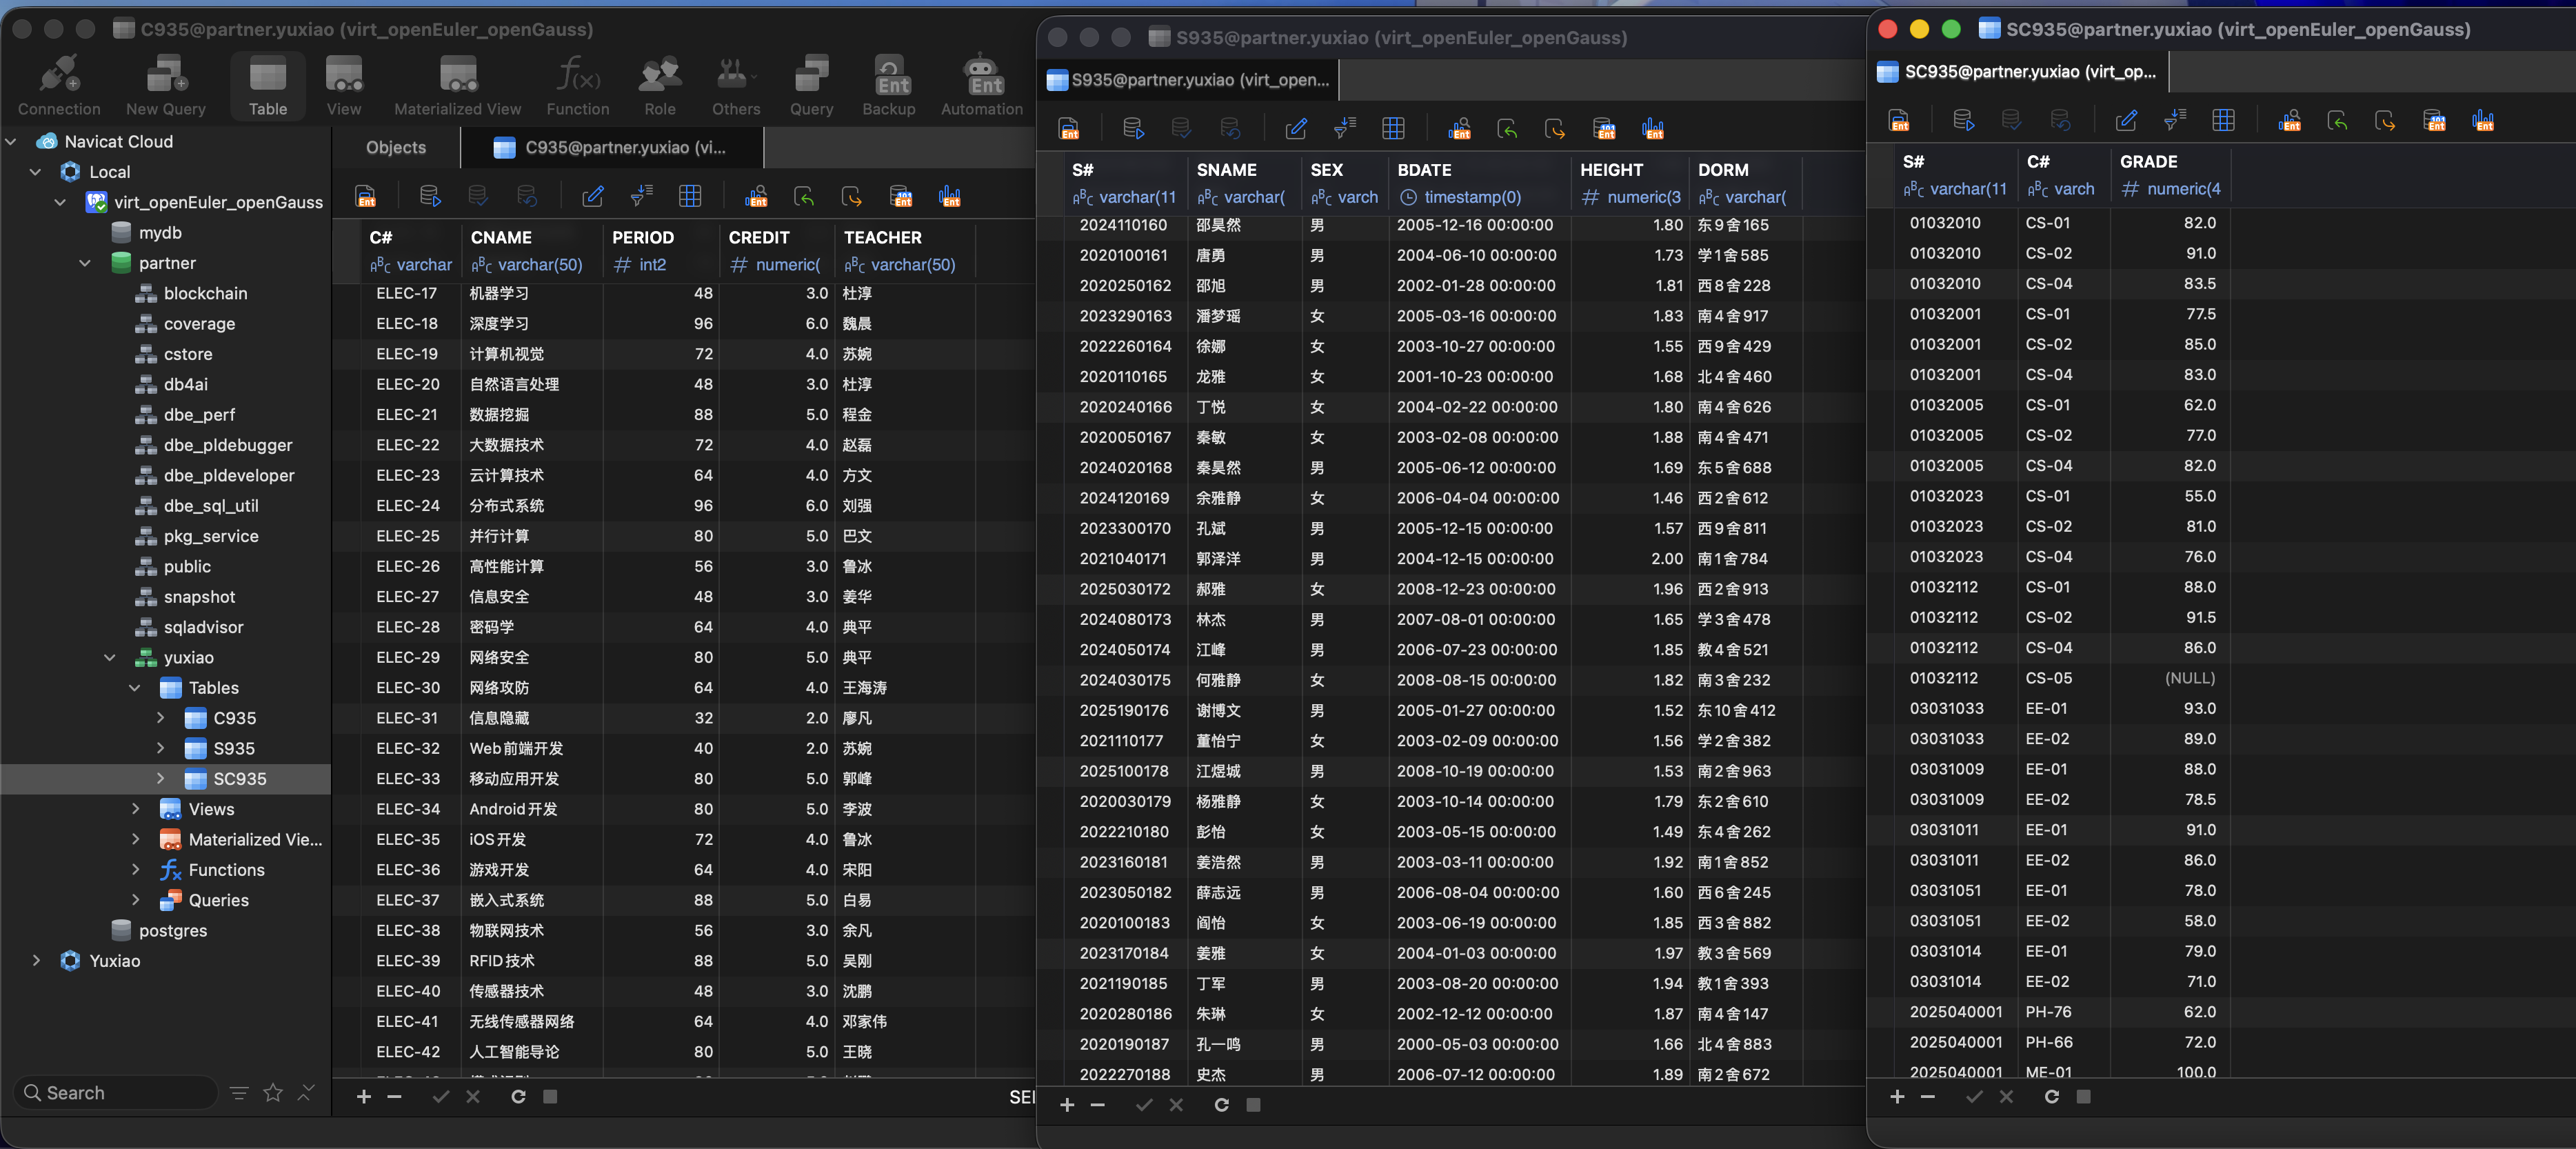
\includegraphics[width=0.88\textwidth]{images/28_5_2.png}
\caption{Navicat 中查看恢复后合作同学的数据库结构与数据内容}
\label{fig:restore_navicat}
\end{figure}

\textbf{恢复结果分析}：从 Navicat 中可以看到，合作同学的数据库恢复完整，表结构设计与本实验基本一致，同样包含学生表、课程表和选课表三张核心表，并遵循了以学号后三位为后缀的命名规则。表的属性设计合理，各字段数据类型选择恰当，数据类型约束符合实验要求。选课数据具有一定规模，各课程的选课分布较为均衡，成绩数据覆盖了不同分段，体现了数据生成的合理性。

\subsection{六、触发器设计——删除记录的自动备份}

\subsubsection{实验目标}

在 SC799 表上设计行级触发器，使每次删除记录时，触发器自动将被删除的记录（含删除时间戳）写入备份表 BK799，实现完整的删除审计日志功能。

\subsubsection{创建备份表 BK799}

BK799 的结构与 SC799 基本一致，额外增加 \texttt{DDATE}（删除时间）字段，类型为 \texttt{TIMESTAMP}：

\begin{lstlisting}[style=sqlstyle]
CREATE TABLE "public"."BK799" (
    "S_num"  VARCHAR(20),
    "C_num"  VARCHAR(20),
    "GRADE"  NUMERIC(4,1),
    "DDATE"  TIMESTAMP
);
\end{lstlisting}

\begin{figure}[H]
\centering
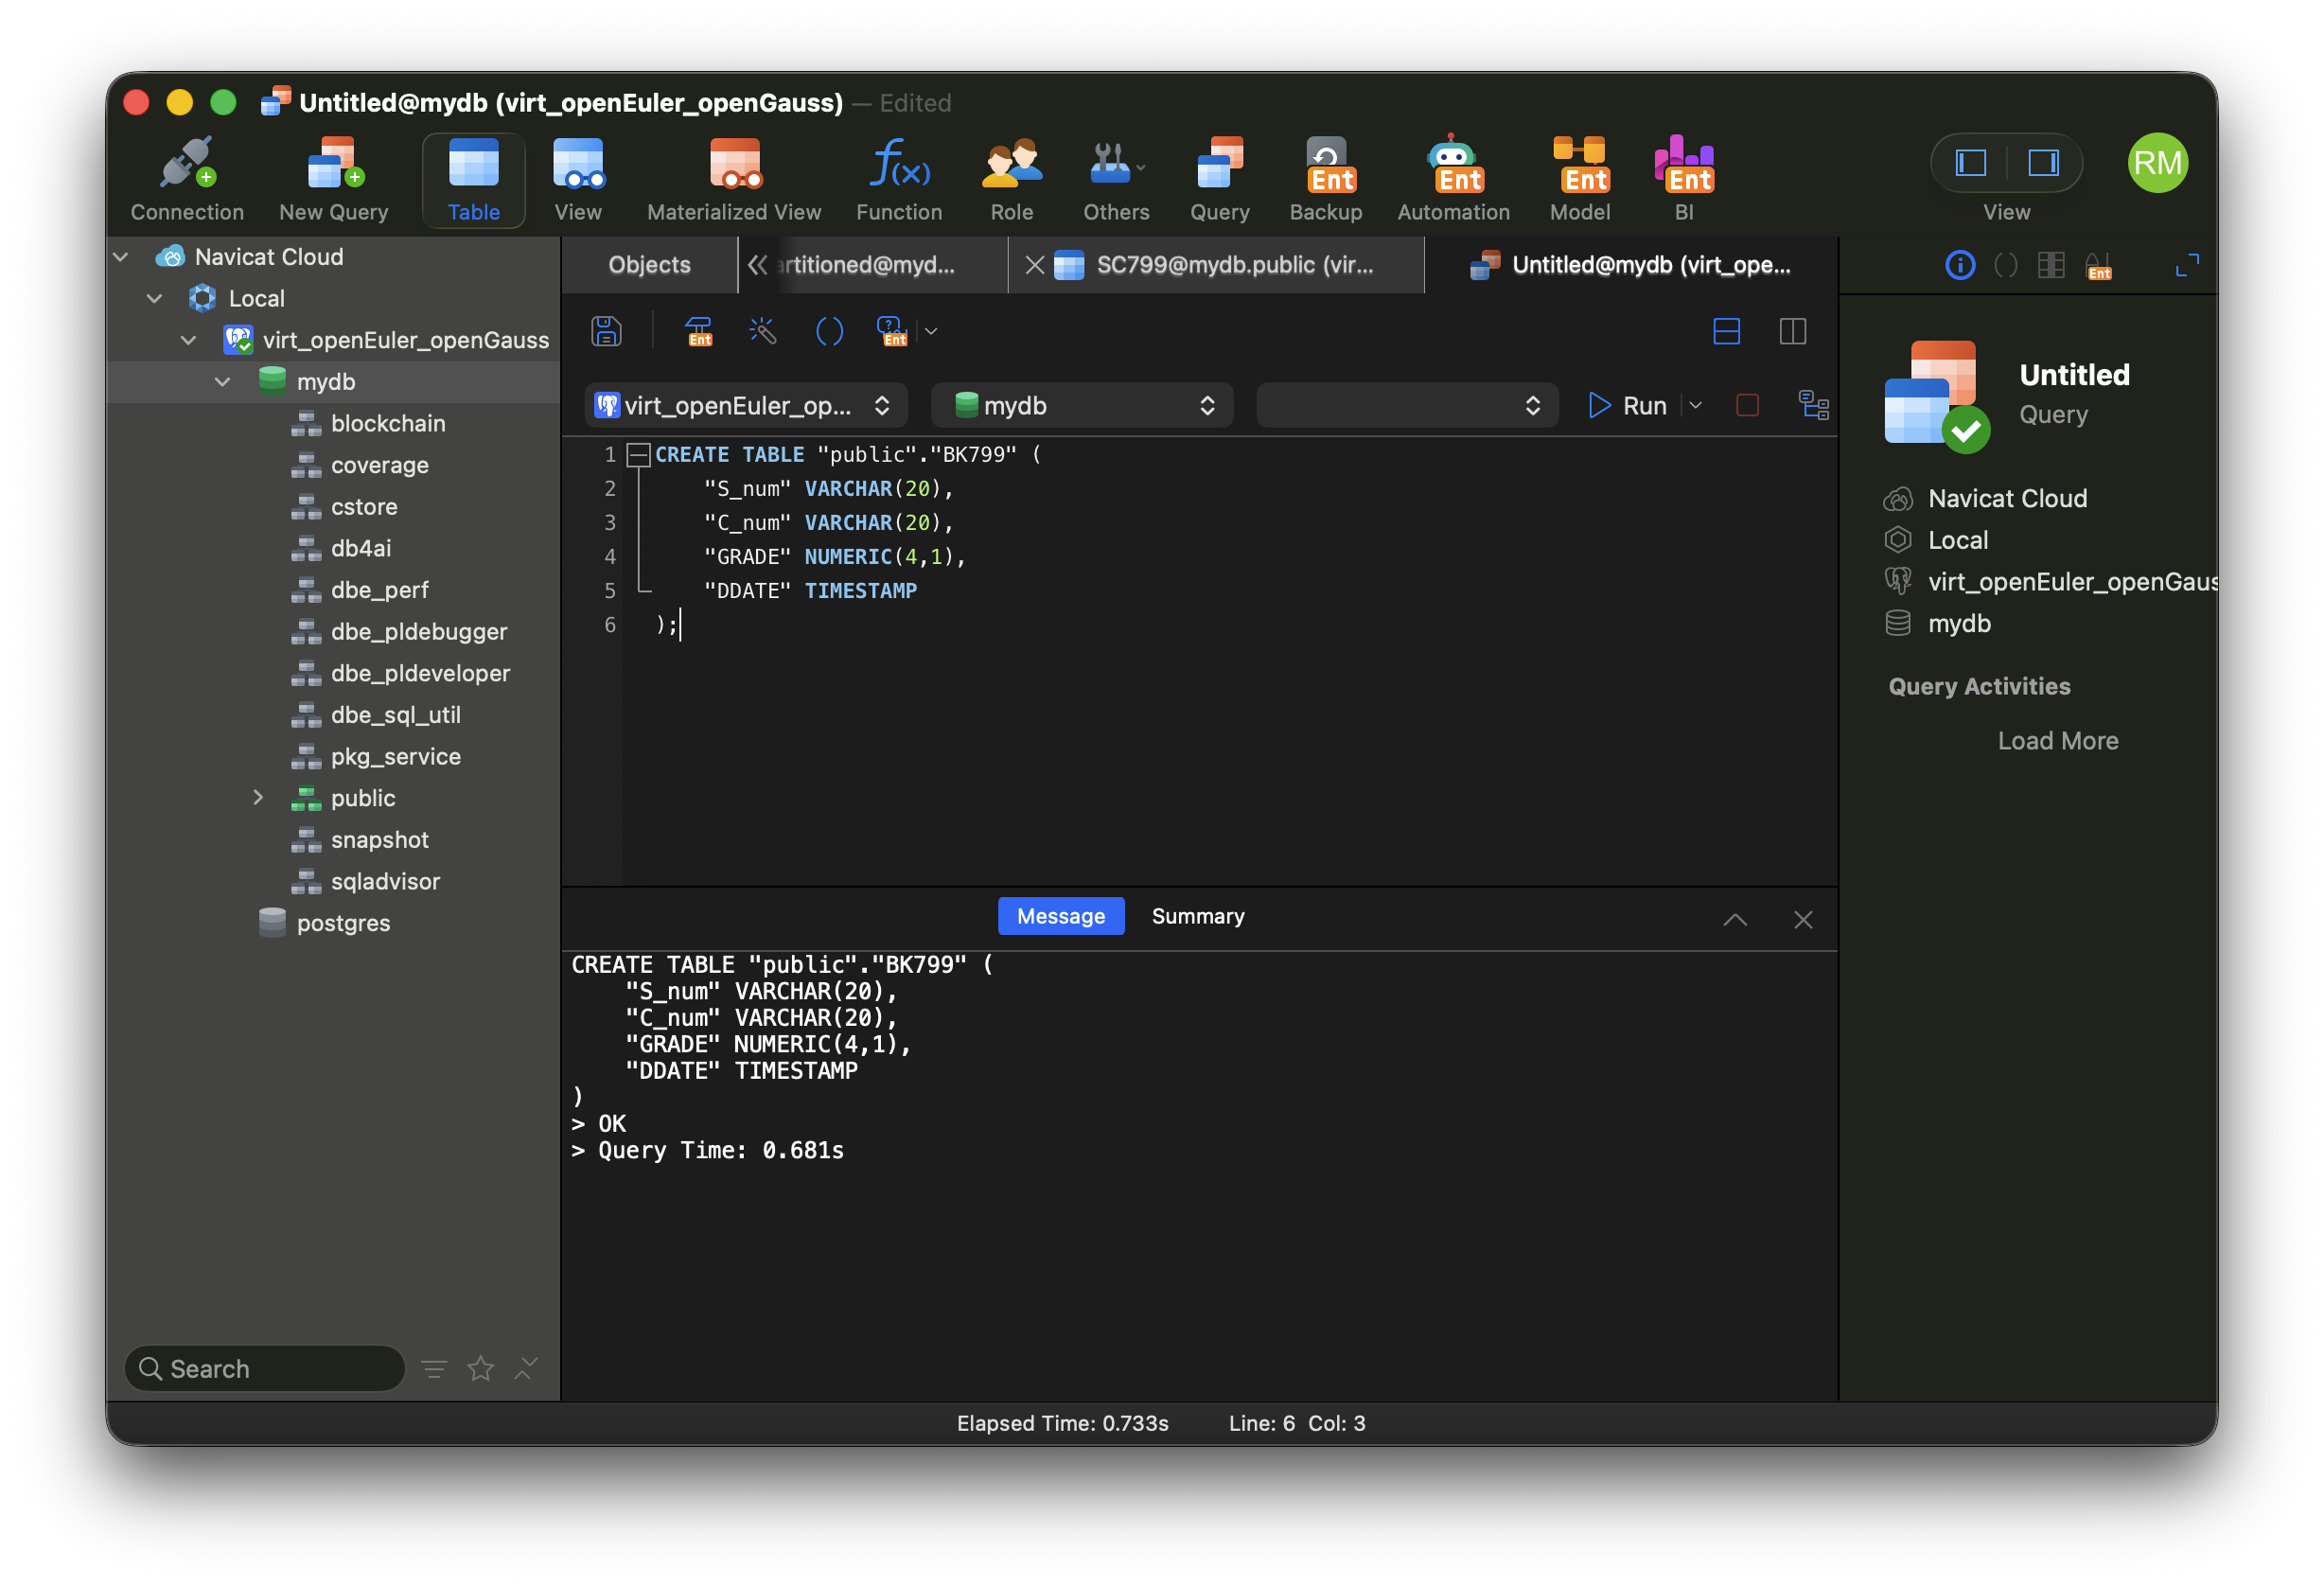
\includegraphics[width=0.88\textwidth]{images/29_6_1.png}
\caption{创建备份表 BK799，包含 S\_num、C\_num、GRADE 及删除时间戳 DDATE 四个字段}
\label{fig:bk799}
\end{figure}

\subsubsection{创建触发器函数与触发器}

openGauss 中触发器由两部分组成：（1）使用 PL/pgSQL 编写的触发器函数，定义触发时执行的逻辑；（2）触发器声明，将函数绑定到指定表的指定事件上。

\begin{lstlisting}[style=sqlstyle]
-- 第 1 步：创建触发器函数
CREATE OR REPLACE FUNCTION log_deleted_sc_record()
RETURNS TRIGGER AS $$
BEGIN
    -- OLD 伪行保存了被删除记录的原始数据
    INSERT INTO "public"."BK799"
        ("S_num","C_num","GRADE","DDATE")
    VALUES (OLD."S_num", OLD."C_num", OLD."GRADE", NOW());
    RETURN OLD;
END;
$$ LANGUAGE plpgsql;

-- 第 2 步：在 SC799 表上创建行级 AFTER DELETE 触发器
CREATE TRIGGER trg_sc_delete_backup
AFTER DELETE ON "public"."SC799"
FOR EACH ROW
EXECUTE PROCEDURE log_deleted_sc_record();
\end{lstlisting}

\begin{figure}[H]
\centering
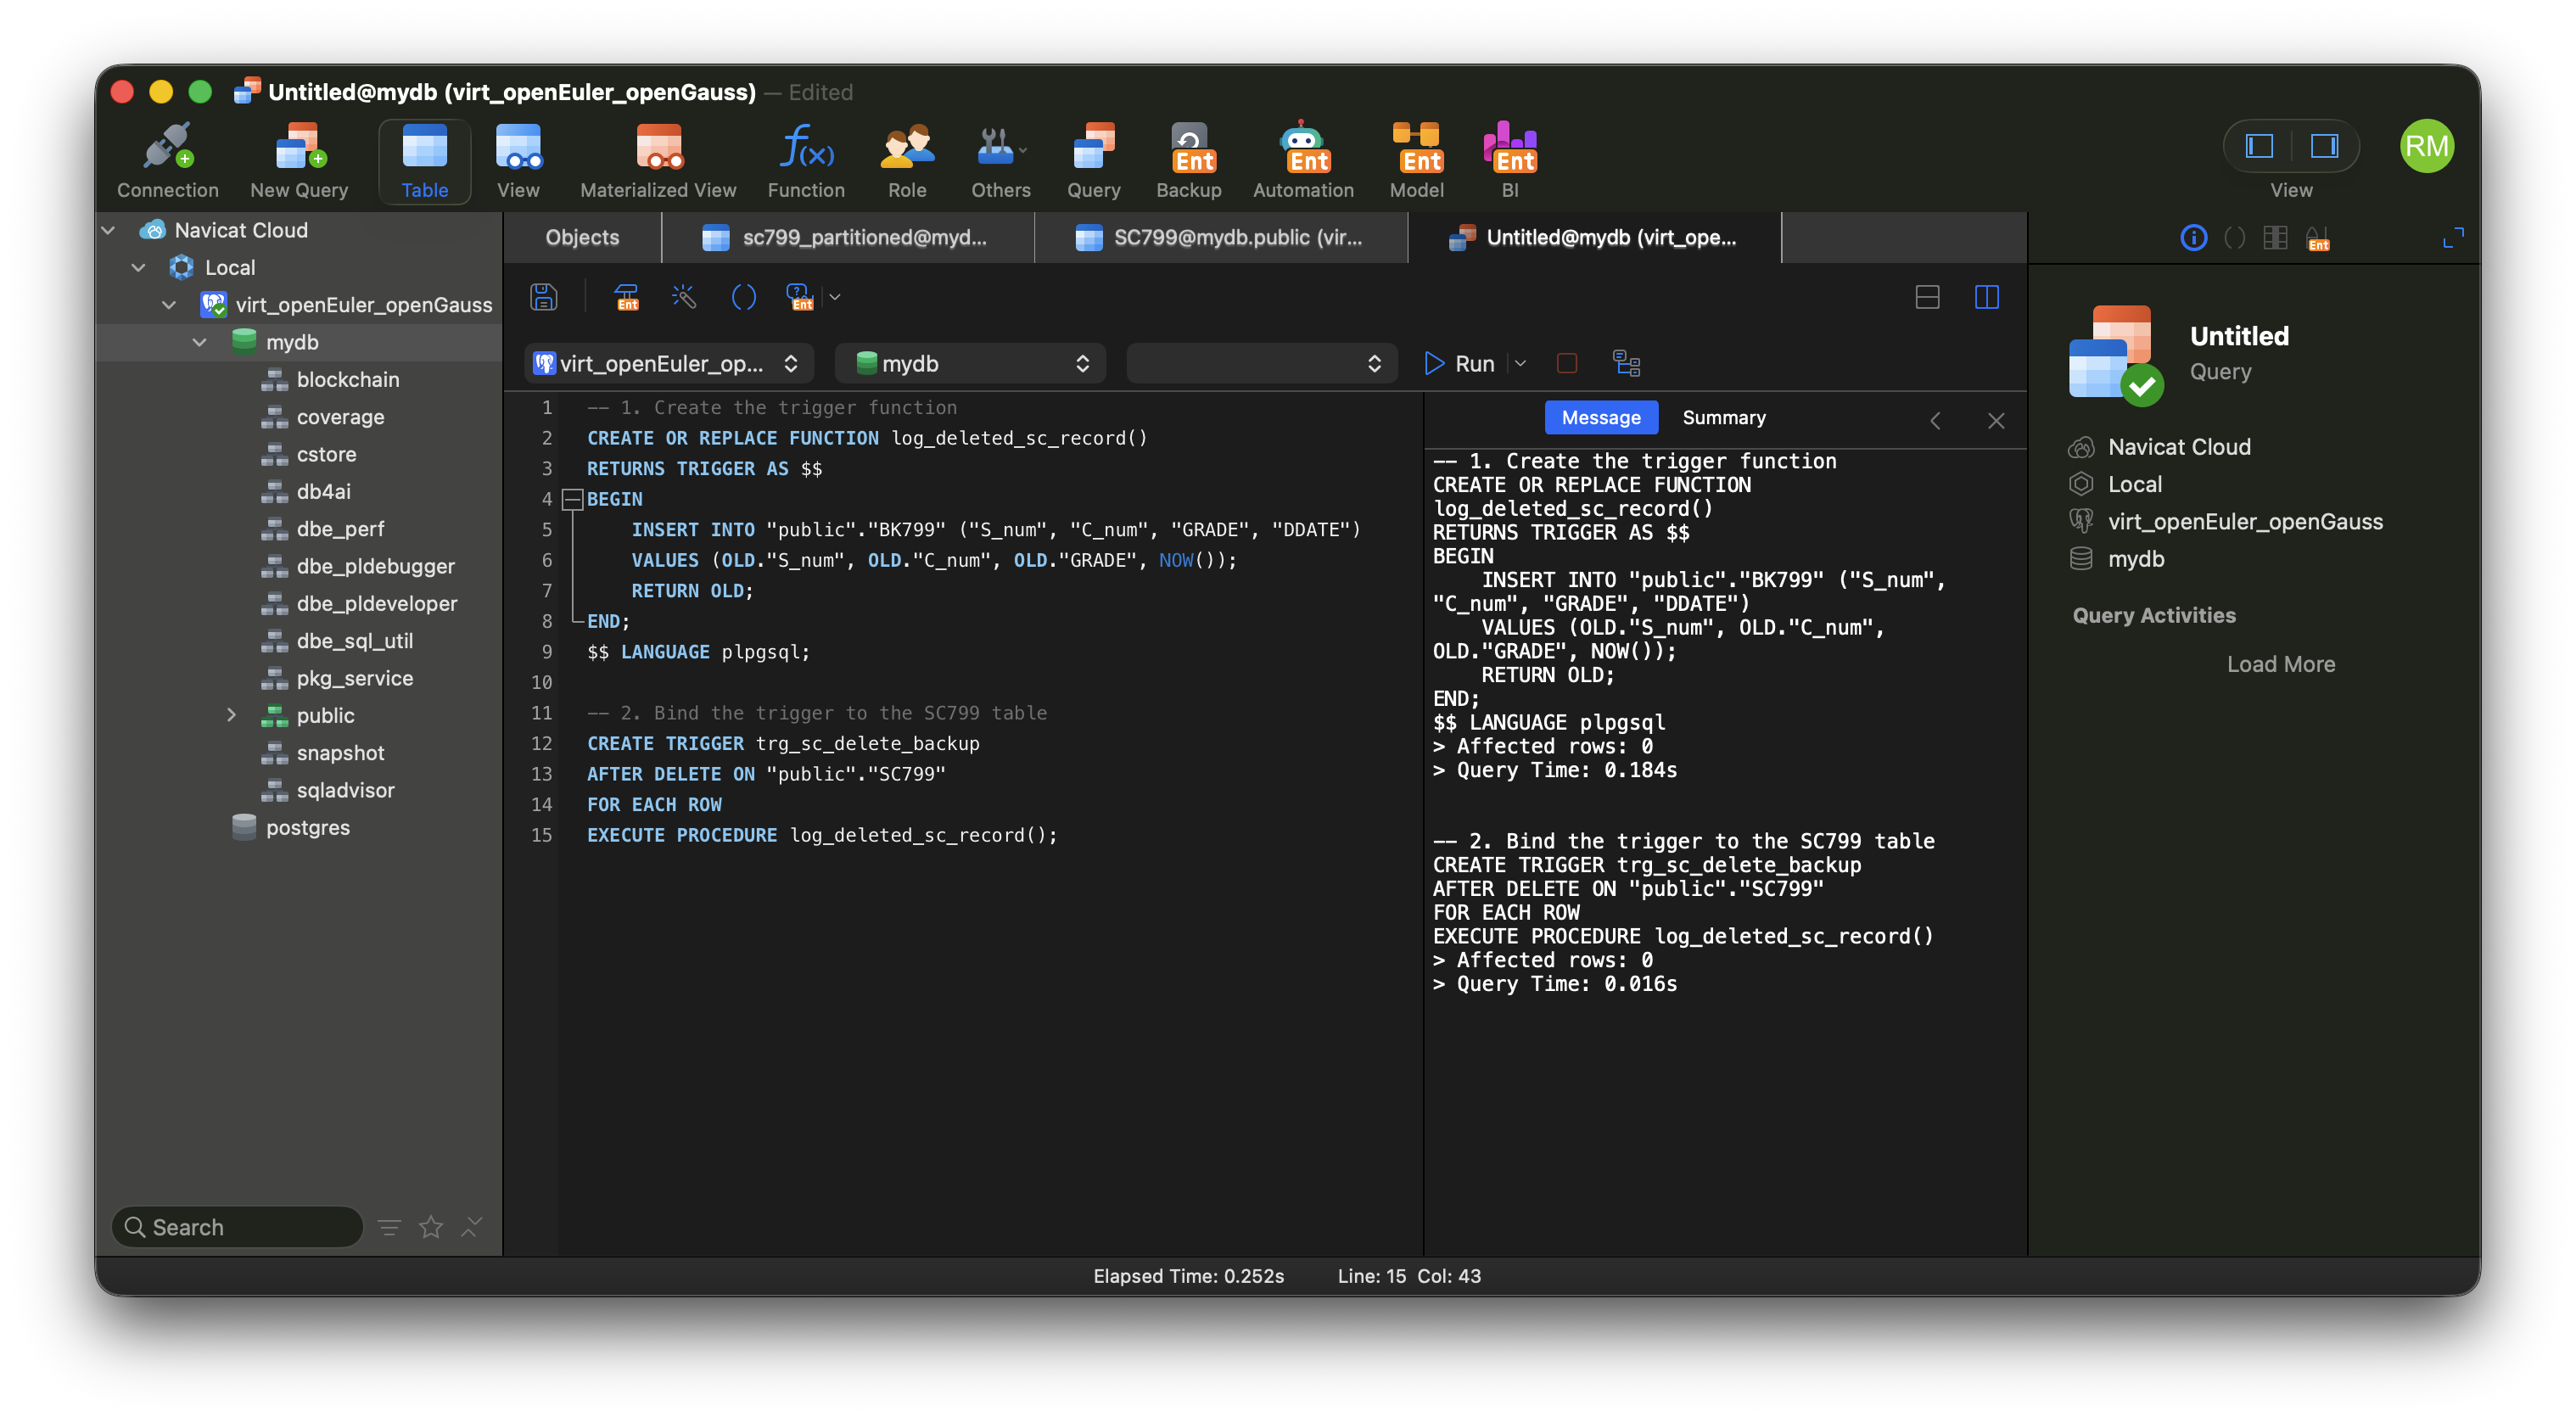
\includegraphics[width=0.88\textwidth]{images/30_6_2.png}
\caption{成功创建 PL/pgSQL 触发器函数及绑定在 SC799 上的行级触发器 trg\_sc\_delete\_backup}
\label{fig:trigger}
\end{figure}

触发器设计要点说明：
\begin{itemize}
  \item \textbf{AFTER DELETE}：在行被实际删除后触发，保证 \texttt{OLD} 伪行中的数据有效。
  \item \textbf{FOR EACH ROW}：行级触发器，每删除一行触发一次，与语句级触发器不同，能精确捕获每一条被删除记录。
  \item \textbf{OLD 伪行}：在 DELETE 触发器中，\texttt{OLD} 包含被删除行的所有字段值，\texttt{NOW()} 函数返回当前精确时间戳（精度至微秒级）。
  \item \textbf{RETURN OLD}：DELETE 触发器的返回值不影响删除结果，但按规范返回 \texttt{OLD}。
\end{itemize}

\subsubsection{Java 程序执行逐条删除以触发触发器}

实验要求由合作同学编写程序连接至数据库，从 SC799 中随机选取 100 条成绩为 NULL 的记录，\textbf{逐条}执行删除。\texttt{TriggerDeletionTask.java} 的实现如下：

\begin{lstlisting}[style=javastyle]
// 第 1 步：随机查询 100 条 NULL 成绩记录
String selectSql =
    "SELECT \"S_num\",\"C_num\" FROM \"public\".\"SC799\" " +
    "WHERE \"GRADE\" IS NULL ORDER BY random() LIMIT 100";

List<SCRef> targets = new ArrayList<>();
try (PreparedStatement sel = conn.prepareStatement(selectSql);
     ResultSet rs = sel.executeQuery()) {
    while (rs.next()) {
        targets.add(new SCRef(rs.getString("S_num"),
                              rs.getString("C_num")));
    }
}

// 第 2 步：逐条删除（每条独立触发一次行级触发器）
String deleteSql =
    "DELETE FROM \"public\".\"SC799\" " +
    "WHERE \"S_num\" = ? AND \"C_num\" = ?";
int deletedCount = 0;
try (PreparedStatement del = conn.prepareStatement(deleteSql)) {
    for (SCRef ref : targets) {
        del.setString(1, ref.sNum);
        del.setString(2, ref.cNum);
        if (del.executeUpdate() > 0) deletedCount++;
    }
}
System.out.println("Deleted " + deletedCount + " records.");
System.out.println("Trigger backed them up into BK799.");
\end{lstlisting}

程序设计关键点：使用\textbf{逐条删除}（循环调用 \texttt{executeUpdate()}）而非批量删除，确保每次 DELETE 都单独触发一次行级触发器，使 BK799 中每条备份记录都携带各自独立的精确删除时间戳。若改用 \texttt{DELETE ... WHERE ... IN (...))} 一次性批量删除，行级触发器虽然也会为每行触发，但在此用逐条的方式更清晰地体现了触发器的行级特性。

\begin{figure}[H]
\centering
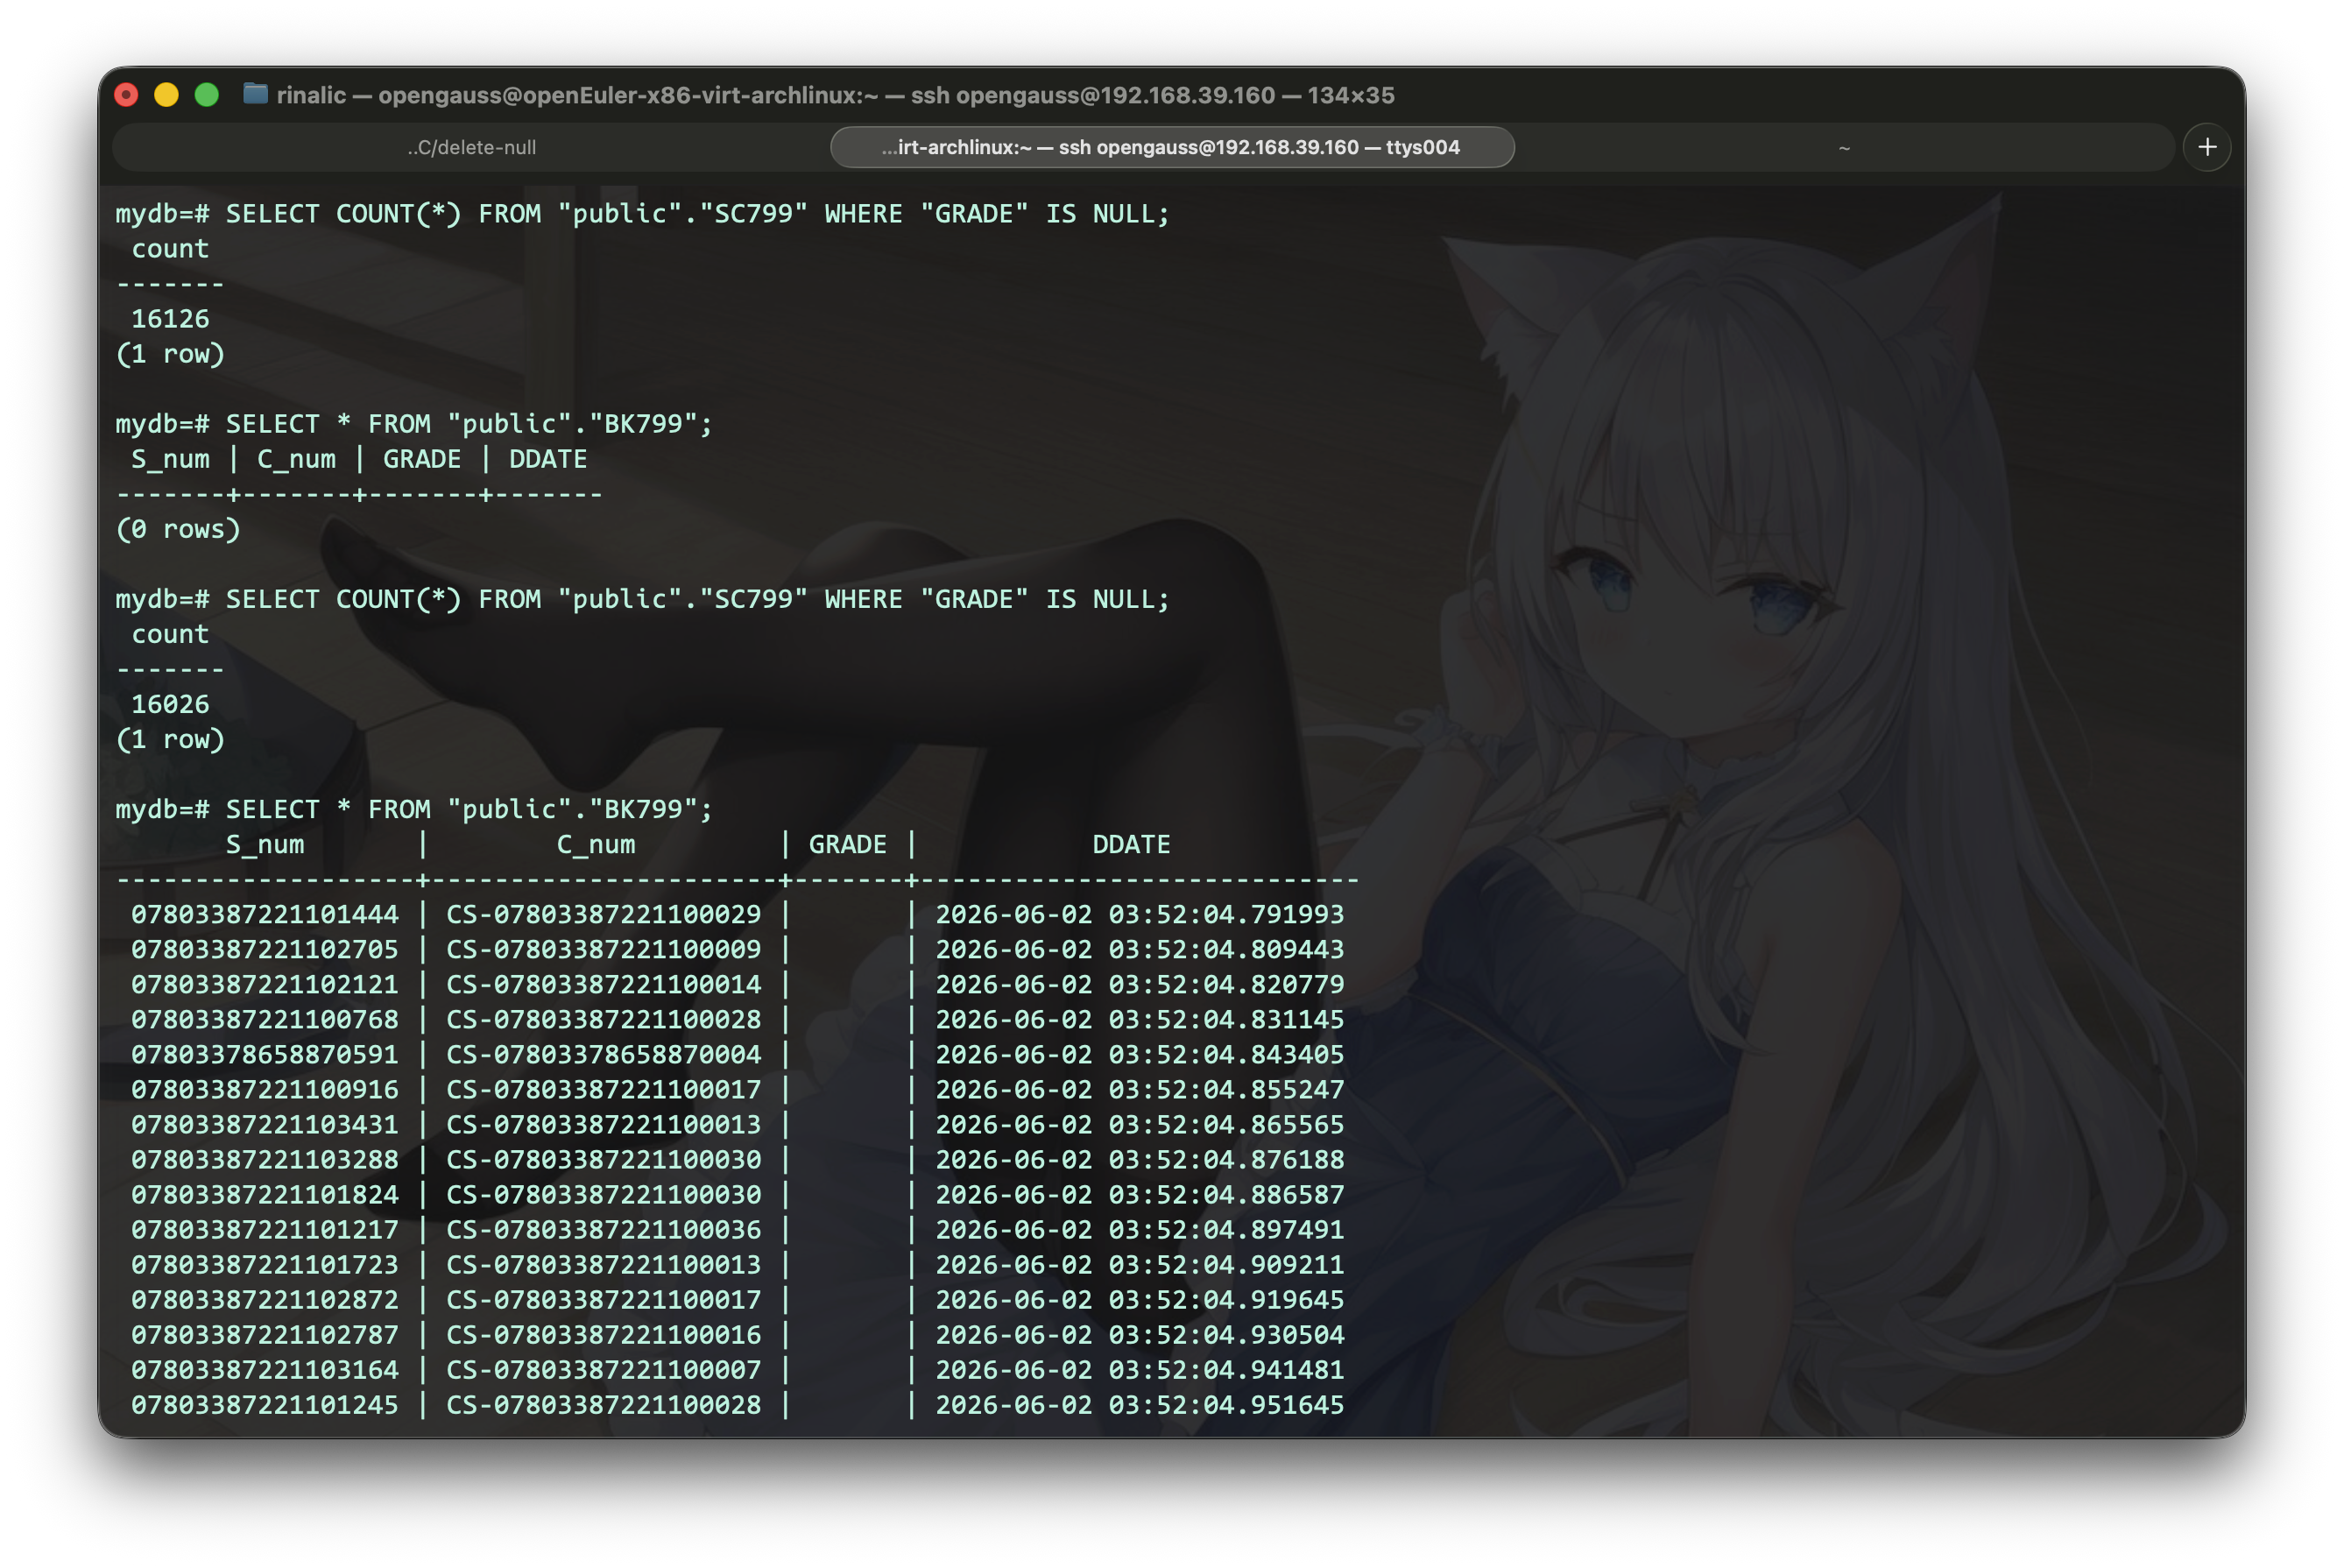
\includegraphics[width=0.90\textwidth]{images/31_6_3.png}
\caption{Java 程序执行前后对比：SC799 中 NULL 成绩记录数量减少，BK799 中出现对应数量的备份记录}
\label{fig:trigger_result}
\end{figure}

执行结果验证：
\begin{itemize}
  \item \textbf{执行前}：查询 \texttt{SELECT COUNT(*) FROM "public"."SC799" WHERE "GRADE" IS NULL} 返回若干行，BK799 为空表。
  \item \textbf{Java 程序执行}：程序连接数据库，随机选取最多 100 条 NULL 成绩记录，逐一调用 DELETE。
  \item \textbf{执行后}：SC799 中 NULL 成绩记录数量相应减少，BK799 中新增对应数量的备份记录，每条记录包含学号、课程编号、成绩（NULL）以及精确到毫秒的删除时间戳 \texttt{DDATE}。不同记录的 \texttt{DDATE} 值各不相同，体现了逐条触发的特性。
\end{itemize}

% ===== 四、实验总结 =====
\section{实验总结}

本实验通过系统性地使用 openGauss 数据库管理系统，完整实践了关系数据库的全链路操作流程，主要收获如下：

\begin{itemize}
  \item \textbf{数据定义与录入}：设计并创建了具有完整约束（主键、外键、类型约束）的三张关系表，合理选择了各属性的数据类型，成功完成了初始数据的录入与系统表属性的查询。

  \item \textbf{复杂 SQL 查询}：编写并验证了 8 条覆盖多表连接、子查询、分组聚合、\texttt{HAVING} 过滤、\texttt{OFFSET} 分页、\texttt{CASE} 表达式等多种技术的查询语句，并通过实际执行结果验证了各查询的正确性。

  \item \textbf{数据库更新操作}：完成了 INSERT、DELETE、UPDATE 操作，观察到主键冲突、条件不匹配等典型边界情形，深刻体会了关系完整性约束在保证数据质量方面的重要性。

  \item \textbf{视图创建}：建立了三个不同语义的视图，理解了视图在封装复杂查询逻辑、简化应用层代码、实现数据访问权限控制方面的价值。

  \item \textbf{大规模 JDBC 编程}：使用 Python 结合 RandomUser API 生成真实感数据，通过 Java 多线程 JDBC 程序批量写入；在实践中掌握了 \texttt{PreparedStatement} 批量提交、多线程连接池、\texttt{ctid} 定向删除等性能优化手段，成功将数据规模扩展至约 20 万行选课记录。

  \item \textbf{查询优化分析}：在 20 万行数据规模下，通过 \texttt{EXPLAIN (ANALYZE, BUFFERS)} 分析了 5 种 SQL 写法的执行计划，理解了优化器在聚合查询场景下倾向于顺序扫描加哈希连接的原因，以及建立索引对不同类型查询的差异化效果。

  \item \textbf{备份与恢复}：成功完成了数据库的多阶段逻辑备份，并恢复了合作同学的数据库，验证了备份文件的完整性与可恢复性。

  \item \textbf{触发器设计}：实现了行级 AFTER DELETE 触发器，配合 Java 程序的逐条删除操作，完整演示了触发器在实现删除审计日志中的应用，深化了对数据库事件驱动机制的理解。
\end{itemize}

% ===== 附录 =====
\section*{附录：核心源代码}

\subsection*{A.1 JDBC 连接测试（ConnectionTestLocal.java）}

\begin{lstlisting}[style=javastyle]
import java.sql.*;
public class ConnectionTestLocal {
    private static final String DEFAULT_URL  =
        "jdbc:opengauss://192.168.39.160:7654/mydb";
    private static final String DEFAULT_USER = "dbremote";
    private static final String DEFAULT_PASSWORD = "dbremote:399";

    public static void main(String[] args) throws Exception {
        String url  = args.length > 0 ? args[0] : DEFAULT_URL;
        String user = args.length > 1 ? args[1] : DEFAULT_USER;
        String pass = args.length > 2 ? args[2] : DEFAULT_PASSWORD;
        Class.forName("org.opengauss.Driver");
        String sql = "SELECT current_database(), current_user, version()";
        try (Connection conn = DriverManager.getConnection(url, user, pass);
             PreparedStatement stmt = conn.prepareStatement(sql);
             ResultSet rs = stmt.executeQuery()) {
            if (rs.next()) {
                System.out.println("Connection successful.");
                System.out.println("Database: "       + rs.getString(1));
                System.out.println("User: "           + rs.getString(2));
                System.out.println("Server version: " + rs.getString(3));
            }
        }
    }
}
\end{lstlisting}

\subsection*{A.2 多线程数据生成（DataGenerator.java 核心片段）}

\begin{lstlisting}[style=javastyle]
// 多线程写入学生数据
private static void generateStudents(int n, int threads,
        long runId, List<String> studentNames)
        throws InterruptedException {
    ExecutorService es = Executors.newFixedThreadPool(threads);
    int batch = 200;
    for (int start = 1; start <= n; start += batch) {
        int s = start, end = Math.min(n, start + batch - 1);
        es.submit(() -> {
            try (Connection conn = DriverManager.getConnection(
                    URL, USER, PASS)) {
                conn.setAutoCommit(false);
                String sql = "INSERT INTO \"public\".\"S799\" "
                    + "(\"S_num\",\"SNAME\",\"SEX\","
                    + "\"BDATE\",\"HEIGHT\",\"DORM\") "
                    + "VALUES (?,?,?,?,?,?)";
                try (PreparedStatement ps = conn.prepareStatement(sql)) {
                    Random rnd = new Random();
                    for (int i = s; i <= end; i++) {
                        String id = String.format("%013d%04d",
                            runId % 1000000000000L, i);
                        String name = pickName(studentNames, i,
                            "Student" + id);
                        ps.setString(1, id);
                        ps.setString(2, name);
                        ps.setString(3, rnd.nextBoolean() ? "男" : "女");
                        // ... 日期、身高、宿舍字段 ...
                        ps.addBatch();
                    }
                    ps.executeBatch();
                }
                conn.commit();
            } catch (SQLException e) { throw new RuntimeException(e); }
        });
    }
    es.shutdown();
    es.awaitTermination(1, TimeUnit.HOURS);
}
\end{lstlisting}

\subsection*{A.3 触发器删除任务（TriggerDeletionTask.java 核心片段）}

\begin{lstlisting}[style=javastyle]
// 随机查询 100 条 NULL 成绩记录并逐条删除
String selectSql = "SELECT \"S_num\",\"C_num\" "
    + "FROM \"public\".\"SC799\" "
    + "WHERE \"GRADE\" IS NULL ORDER BY random() LIMIT 100";
String deleteSql = "DELETE FROM \"public\".\"SC799\" "
    + "WHERE \"S_num\" = ? AND \"C_num\" = ?";

List<SCRef> targets = new ArrayList<>();
try (PreparedStatement sel = conn.prepareStatement(selectSql);
     ResultSet rs = sel.executeQuery()) {
    while (rs.next())
        targets.add(new SCRef(rs.getString("S_num"),
                              rs.getString("C_num")));
}

int deletedCount = 0;
try (PreparedStatement del = conn.prepareStatement(deleteSql)) {
    for (SCRef ref : targets) {
        del.setString(1, ref.sNum);
        del.setString(2, ref.cNum);
        if (del.executeUpdate() > 0) deletedCount++;
    }
}
System.out.println("Deleted " + deletedCount + " records one by one.");
System.out.println("Trigger backed them up into BK799.");
\end{lstlisting}

\subsection*{A.4 运行命令汇总}

\begin{verbatim}
# JDBC 连接测试
javac -cp "opengauss-jdbc-6.0.0.jar" ConnectionTestLocal.java
java  -cp ".:opengauss-jdbc-6.0.0.jar" ConnectionTestLocal

# Python 数据名称生成
pip install requests
python generate_names.py --students 1000 --courses 100 \
    --enrollments 20000 --outdir ./sql_out

# 多线程数据生成（四-1 规模）
javac -cp "../opengauss-jdbc-6.0.0.jar" DataGenerator.java
java  -cp ".:../opengauss-jdbc-6.0.0.jar" DataGenerator \
    --students 1000 --courses 100 --enrollments 20000 --threads 8

# 大规模数据生成（四-2 规模）
java  -cp ".:../opengauss-jdbc-6.0.0.jar" DataGenerator --task2

# 查询优化实验（建立索引 + 运行 EXPLAIN ANALYZE）
pip install psycopg2-binary sqlparse
python optimization_driver.py \
    --host 192.168.39.160 --port 7654 --dbname mydb \
    --user dbremote --password 'dbremote:399' \
    --apply-indexes --run-queries --repeats 3 --analyze-after-ddl

# 触发器验证删除任务
javac -cp "../opengauss-jdbc-6.0.0.jar" TriggerDeletionTask.java
java  -cp ".:../opengauss-jdbc-6.0.0.jar" TriggerDeletionTask
\end{verbatim}

\end{document}
